% =============================================================================
% Розділ 3. Результати експериментів та їх оцінка
% Підключення: % =============================================================================
% Розділ 3. Результати експериментів та їх оцінка
% Підключення: % =============================================================================
% Розділ 3. Результати експериментів та їх оцінка
% Підключення: % =============================================================================
% Розділ 3. Результати експериментів та їх оцінка
% Підключення: \input{sections/section3_experiments}
% =============================================================================
\providecommand{\px}{пкс}
\providecommand{\code}[1]{\texttt{#1}}

\newpage
\section{Результати експериментів та їх оцінка}
\label{sec:experiments}

\subsection{Методика експериментального дослідження}

\textbf{Дані та обладнання.}\\
Усі експерименти виконано на даних, описаних у розділі~\ref{sec:implementation}: ортофотоплан $6200 \times 4320$~пікселів, розбитий на 384 фрагменти $512 \times 512$ з перекриттям 50\,\%, і 95 кадрів відео польоту БпЛА з частотою 1~кадр/с. Обчислення виконано на GPU NVIDIA GeForce GTX 1650. Якщо не зазначено інше, використано параметри за замовчуванням: $s_f = 0{,}27$, $k = 1$, поріг RANSAC 3~\px{}, мінімум 15 геометрично узгоджених відповідностей.

\textbf{Досліджувані конфігурації.}\\
Порівнювалися чотири конфігурації системи --- поєднання методу зіставлення (LightGlue або LoFTR) та оцінювача гомографії (RANSAC або MAGSAC++). Решта етапів (масштабування, геометрична перевірка, фільтр і ранжування, трекер, компенсація курсу) для всіх конфігурацій однакові. Це забезпечує коректність порівняння: на відміну від курсової роботи, обидва методи отримують зображення однакового масштабу.

\textbf{Метрики зіставлення.}\\
Для пари <<кадр --- фрагмент>> використовуються:
\begin{itemize}
    \item $N_{\text{all}}$ --- кількість відповідностей, які повернув метод;
    \item $N_{\text{in}}$ --- кількість геометрично узгоджених відповідностей (похибка репроєкції не більша за поріг RANSAC);
    \item $r = N_{\text{in}} / N_{\text{all}}$ --- частка геометрично узгоджених відповідностей;
    \item $\bar{e}$ --- середня похибка репроєкції геометрично узгоджених відповідностей, \px{}. За побудовою вона не перевищує порогу RANSAC, тому характеризує точність відповідностей, а не успішність локалізації;
    \item час обробки, с.
\end{itemize}

\textbf{Метрики локалізації.}\\
Похибка локалізації кадру $i$ визначається відносно еталонного положення (п.~\ref{sec:gt}):
\begin{equation}
E_i = \sqrt{(X_i - X_i^{\text{ет}})^2 + (Y_i - Y_i^{\text{ет}})^2}, \quad \text{\px{}}.
\end{equation}
За сукупністю кадрів обчислюються середня, медіанна та максимальна похибка, середньоквадратична похибка $\text{RMSE} = \sqrt{\tfrac{1}{N}\sum_i E_i^2}$, 90-й процентиль $P_{90}$, а також частка успішних локалізацій
\begin{equation}
\text{Success@}K = \frac{\left|\{ i : E_i \le K \}\right|}{N}, \qquad K \in \{10, 25, 50\}~\text{\px{}},
\end{equation}
де $N$ --- кількість усіх кадрів з еталоном; кадри, для яких система не видала положення, вважаються неуспішними. Ортофотоплан не має просторової прив'язки, тому похибки наведено в пікселях карти і в метри не переводяться.

\subsection{Еталонні координати}
\label{sec:gt}

Для обчислення похибки локалізації потрібне еталонне положення кадру, незалежне від системи, що оцінюється. Використання як еталона результатів самої системи або їхнього візуального <<уточнення>> призвело б до заниженої оцінки похибки, тому еталон побудовано за ручними відповідностями точок.

\textbf{Процедура розмітки.}\\
Для опорного кадру оператор у спеціально розробленому інструменті вказує щонайменше 5 пар відповідних точок <<кадр $\leftrightarrow$ карта>>, розташованих на рівні землі (кути дорожньої розмітки та бордюрів, перехрестя доріжок, основи стовпів). Дахи будівель не використовуються, оскільки через паралакс вони зміщені відносно земної поверхні. За всіма парами методом найменших квадратів (без RANSAC) оцінюється гомографія $H_{\text{ет}}$, і центр кадру переноситься на карту. Приклад розмітки наведено на рисунку~\ref{fig:gt-example}.

\begin{figure}[H]
    \centering
    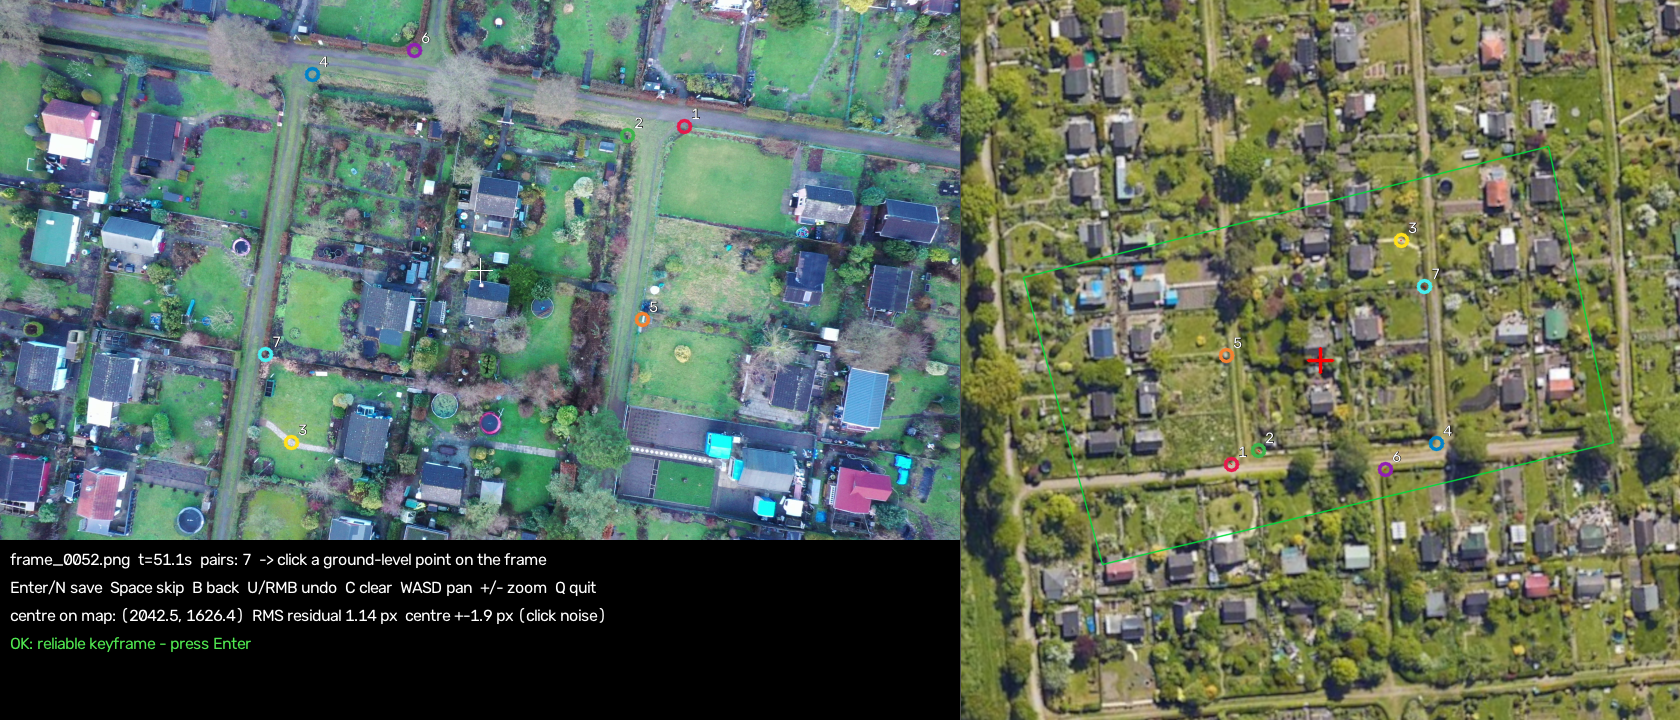
\includegraphics[width=\linewidth]{images/master/gt_annotation_example.png}
    \caption{Розмітка еталонного положення кадру 52 (кадр повернутий на $\approx 170^\circ$ відносно карти): пари точок пронумеровано, зеленим --- спроєктований контур кадру, червоним хрестиком --- центр кадру}
    \label{fig:gt-example}
\end{figure}

\textbf{Контроль якості розмітки.}\\
З чотирьох пар гомографія визначається точно, тому залишкова похибка дорівнює нулю й не дає змоги виявити помилку оператора. У першій версії розмітки саме такі кадри (по 4 пари, скупчені в одній частині кадру) давали <<похибку>> системи понад 100~\px{} для всіх методів одночасно. Тому опорний кадр вважається надійним, якщо:
\begin{enumerate}
    \item вказано не менше 5 пар;
    \item залишкова похибка кожної пари не перевищує 3~\px{}, інакше одна з точок хибна;
    \item 95-й процентиль зміщення центру за випадкового шуму кліків ($\sigma = 2$~пікселі кадру та 1~піксель карти, метод Монте-Карло) не перевищує 5~\px{}, інакше точки скупчені або центр кадру розташований далеко від них.
\end{enumerate}
Критерій не використовує результатів системи. Опорні кадри обрано візуально так, щоб на них були чіткі наземні орієнтири і щоб вони рівномірно покривали політ, включно з розворотами. Кадри над пустирем (33--40) і каналом (66--69) пропущено через відсутність надійних точок.

Розмічено 19 опорних кадрів, з них 18 надійних: 5--8 пар на кадр (у середньому 6,2), медіанна невизначеність центру 2,6~\px{} (максимум 5,0~\px{}), найбільша залишкова похибка пари --- 3,0~\px{}. Ненадійний кадр 40 (пустир, 4 пари) в метрики не включено. Для 7 надійних кадрів центр кадру лежить поза областю вказаних точок, тобто його положення екстрапольовано. Шум кліків цим критерієм враховано, але систематичні похибки (дисторсія ширококутного об'єктива, паралакс) за межами точок не оцінюються, що слід мати на увазі під час аналізу окремих кадрів.

Для кадрів між опорними еталон можна лінійно інтерполювати в часі, однак на розворотах інтерполяція <<зрізає>> траєкторію. Через це похибка за інтерпольованим еталоном вимірює насамперед похибку інтерполяції: для всіх чотирьох конфігурацій вона однакова, $\approx 38$~\px{}. Тому всі наведені нижче похибки обчислено лише за 18 надійними опорними кадрами.

\subsection{Зіставлення кадру з відомим фрагментом карти}
\label{sec:exp-pair}

\textbf{Результати для еталонної пари.}\\
Для перевірки конвеєра використано пару з курсової роботи: кадр 2 і фрагмент карти, що містить місце зйомки (результати --- у табл.~\ref{tab:pair}, приклади відповідностей --- на рис.~\ref{fig:pair}).

\begin{table}[H]
\centering
\caption{Зіставлення еталонної пари <<кадр 2 --- фрагмент 196>> (GPU, медіана часу з 5 запусків)}
\label{tab:pair}
\begin{tabular}{lcccccc}
\toprule
\textbf{Метод} & $N_{\text{all}}$ & $N_{\text{in}}$ & $r$ & $\bar{e}$, \px{} & масштаб $\sigma$ & час, с \\
\midrule
LightGlue & 310 & 89 & 0,29 & 1,58 & 0,267 & 0,25 \\
LoFTR & 631 & 184 & 0,29 & 1,40 & 0,202 & 0,27 \\
\bottomrule
\end{tabular}
\end{table}

\begin{figure}[H]
    \centering
    \begin{subfigure}{\linewidth}
        \centering
        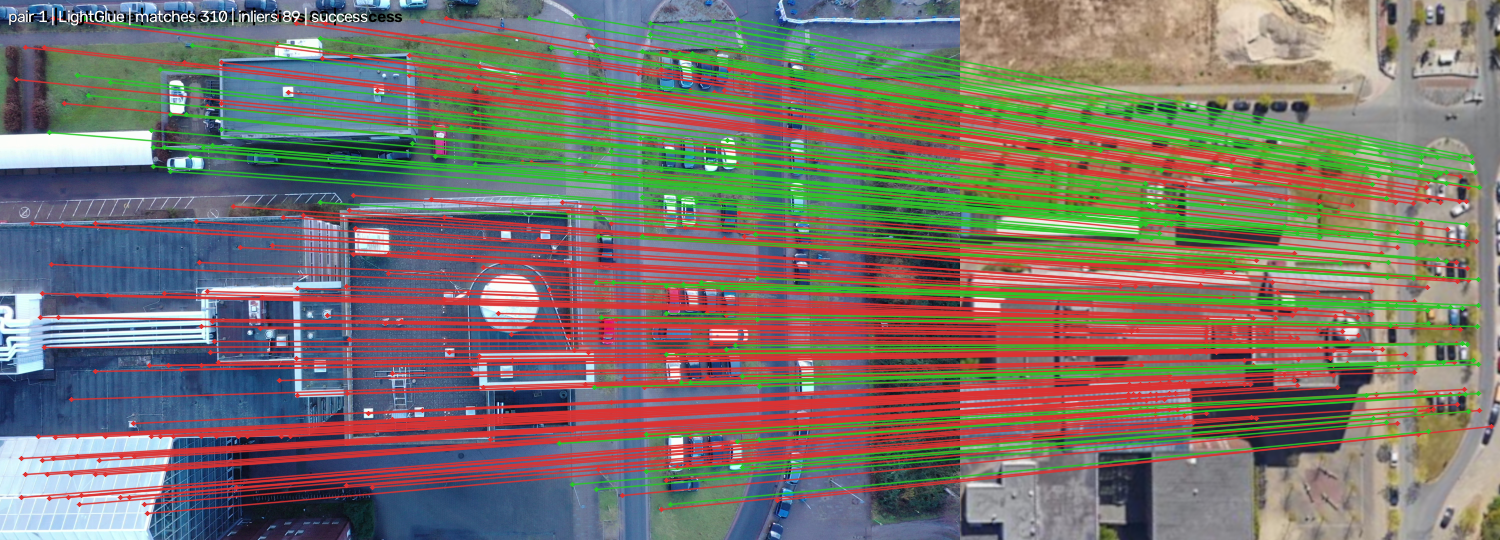
\includegraphics[width=0.92\linewidth]{images/master/pair_lightglue_matches.png}
        \caption{LightGlue}
    \end{subfigure}
    \vspace{2mm}
    \begin{subfigure}{\linewidth}
        \centering
        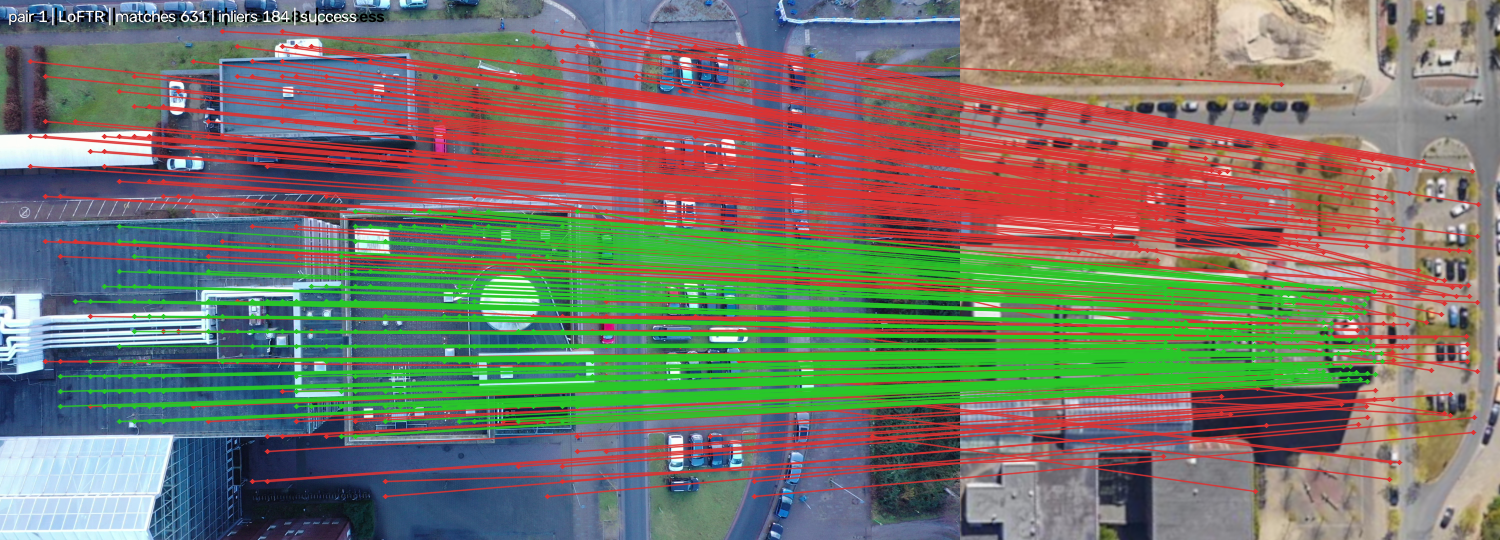
\includegraphics[width=0.92\linewidth]{images/master/pair_loftr_matches.png}
        \caption{LoFTR}
    \end{subfigure}
    \caption{Відповідності між кадром 2 (ліворуч) і фрагментом карти (праворуч): зеленим --- геометрично узгоджені, червоним --- відкинуті RANSAC}
    \label{fig:pair}
\end{figure}

\textbf{Виправлення методики курсової роботи.}\\
У курсовій роботі на цій парі LightGlue мав 229 геометрично узгоджених відповідностей проти 117 у LoFTR і працював повільніше (6,55~с проти 4,18~с). Аналіз прототипу показав, що ці результати отримано за нерівних умов. По-перше, SuperPoint неявно масштабував вхідні зображення до 1024~пікселів, тоді як LoFTR працював із 512. По-друге, обидва методи бачили лише центральну квадратну частину кадру, без нормалізації масштабу. По-третє, час вимірювався без прогрівання моделей. За однакових умов (табл.~\ref{tab:pair}) співвідношення змінюється: LoFTR знаходить удвічі більше геометрично узгоджених відповідностей за однакової їх частки, а час обробки пари на GPU для обох методів становить $\approx 0{,}25$~с. Тому числові результати курсової роботи надалі не використовуються.

\textbf{Калібрування масштабу кадру.}\\
Початкову оцінку $s_f \approx 0{,}25$ отримано вручну. Для її уточнення кадр 2 зіставлено з фрагментом карти $1024 \times 1024$, що повністю містить контур кадру. Обидва методи за обох оцінювачів і робочих масштабів $k \in \{1;\, 1{,}5\}$ дали узгоджений масштаб гомографії $\sigma = 0{,}267$--$0{,}277$, а оцінки центра кадру розійшлися не більше ніж на 16~\px{}. Отже, прийнято $s_f = 0{,}27$: кадр $1920 \times 1080$ покриває на карті ділянку $\approx 518 \times 292$~\px{}, ширшу за фрагмент 512~\px{}.

\textbf{Вплив непланарності сцени.}\\
На фрагменті 196 масштаб гомографії LoFTR ($\sigma = 0{,}20$) суттєво менший за калібрувальний (табл.~\ref{tab:pair}). Геометрично узгоджені відповідності LoFTR зосереджені на даху високої будівлі, ближчому до камери, ніж земля, тому RANSAC оцінює гомографію площини даху, а не площини землі (рис.~\ref{fig:pair}б). Центр кадру при цьому все одно визначається з похибкою $\approx 15$~\px{}, оскільки він сам розташований на цьому даху. Цей ефект є прямим наслідком припущення про плоску сцену.

\textbf{Контрольна перевірка на хибних фрагментах.}\\
Кадр 2 зіставлено з 33 фрагментами, серед яких є як сусідні до місця зйомки, так і віддалені. Фрагменти, що не перетинаються з кадром, дали щонайбільше 15 (LightGlue) і 14 (LoFTR) геометрично узгоджених відповідностей і всі були відкинуті: частина за порогом $N_{\text{in}} \ge 15$, частина --- перевіркою правдоподібності гомографії. Усі фрагменти, що перетинаються з кадром, дали від 18 до 240 таких відповідностей і пройшли перевірку. Запас між цими групами невеликий, тому для вибору фрагмента додатково використовуються частка відповідностей і умова потрапляння центра кадру у фрагмент (п.~\ref{sec:search}).

\subsection{Автоматичний пошук фрагмента для одиночного кадру}

Для кадру 2 виконано пошук без будь-якої інформації про місце зйомки (табл.~\ref{tab:search}, рис.~\ref{fig:global-loc}).

\begin{table}[H]
\centering
\caption{Автоматичний пошук фрагмента для кадру 2}
\label{tab:search}
\small
\begin{tabular}{lccccc}
\toprule
\textbf{Запуск} & \textbf{Перевірено} & \textbf{Пройшли фільтр} & \textbf{Переможець} & \textbf{Центр $(X, Y)$, \px{}} & \textbf{Час, с} \\
\midrule
LightGlue, уся карта, кеш & 384 & 5 & 220 & (1121,4;\ 2344,7) & 33 \\
LoFTR, обмежена область & 56 & 5 & 197 & (1108,6;\ 2327,5) & 18 \\
LoFTR, кожен 2-й рядок і стовпець & 96 & 1 & 197 & (1108,6;\ 2327,5) & 32 \\
\bottomrule
\end{tabular}
\end{table}

\begin{figure}[H]
    \centering
    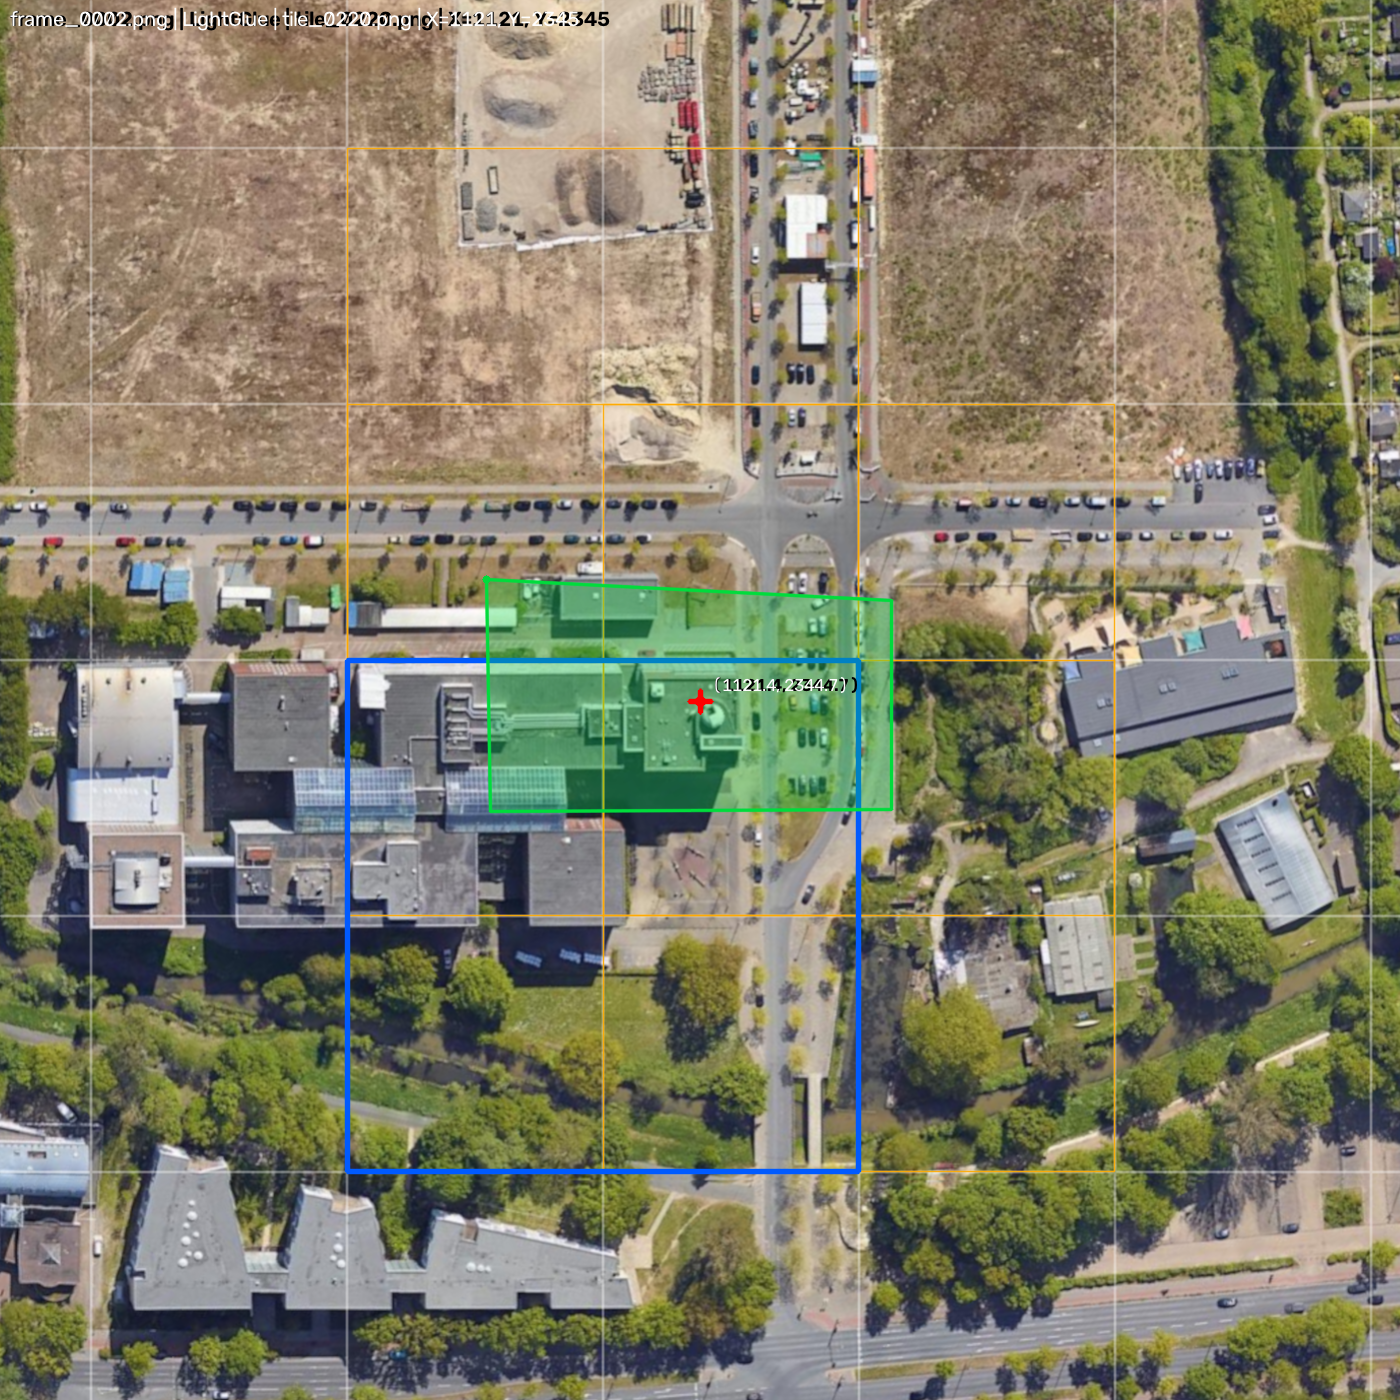
\includegraphics[width=0.75\linewidth]{images/master/global_loc_zoom.png}
    \caption{Результат автоматичного пошуку для кадру 2: сітка перевірених фрагментів, фрагменти, що пройшли фільтр (помаранчеві), фрагмент-переможець (синій), контур огляду камери (зелений) і центр кадру (червоний)}
    \label{fig:global-loc}
\end{figure}

В обох випадках переможцем став фрагмент, суміжний з еталонним фрагментом 196, який також містить центр кадру. Оцінка LoFTR відрізняється від калібрувальної оцінки $\approx(1110;\ 2330)$ на $\approx 3$~\px{}, оцінка LightGlue --- на $\approx 19$~\px{}. Усі фрагменти, що пройшли фільтр, перетинаються з місцем зйомки; жоден віддалений фрагмент фільтр не пройшов. Перегляд усієї карти з кешем ознак займає 33~с (85~мс на фрагмент), що прийнятно для початкової ініціалізації, але не для обробки кожного кадру. Це обґрунтовує використання трекера.

\subsection{Локалізація послідовності кадрів і вплив компенсації курсу}
\label{sec:exp-yaw}

Траєкторія польоту являє собою облітання кварталу: на північ, схід, південь і захід. Під час польоту курс змінюється приблизно так: $0^\circ \to 90^\circ \to 175^\circ \to -90^\circ \to -40^\circ$. Щоб оцінити внесок компенсації курсу, трекер (LightGlue + RANSAC) запущено на всіх 95 кадрах з компенсацією та без неї (табл.~\ref{tab:yaw}, рис.~\ref{fig:yaw}).

\begin{table}[H]
\centering
\caption{Вплив компенсації курсу на трекінг послідовності (LightGlue + RANSAC, 95 кадрів)}
\label{tab:yaw}
\begin{tabular}{lcc}
\toprule
& \textbf{Без компенсації} & \textbf{З компенсацією} \\
\midrule
\textsc{initialized} / \textsc{tracking} / \textsc{interpolated} / \textsc{lost} & 1 / 17 / 3 / 74 & 1 / 94 / 0 / 0 \\
Супровід утрачено & на кадрі 19, не відновлено & ні \\
Загальний час обробки & $\approx 41$~хв & 133~с \\
\bottomrule
\end{tabular}
\end{table}

\begin{figure}[H]
    \centering
    \begin{subfigure}{0.49\linewidth}
        \centering
        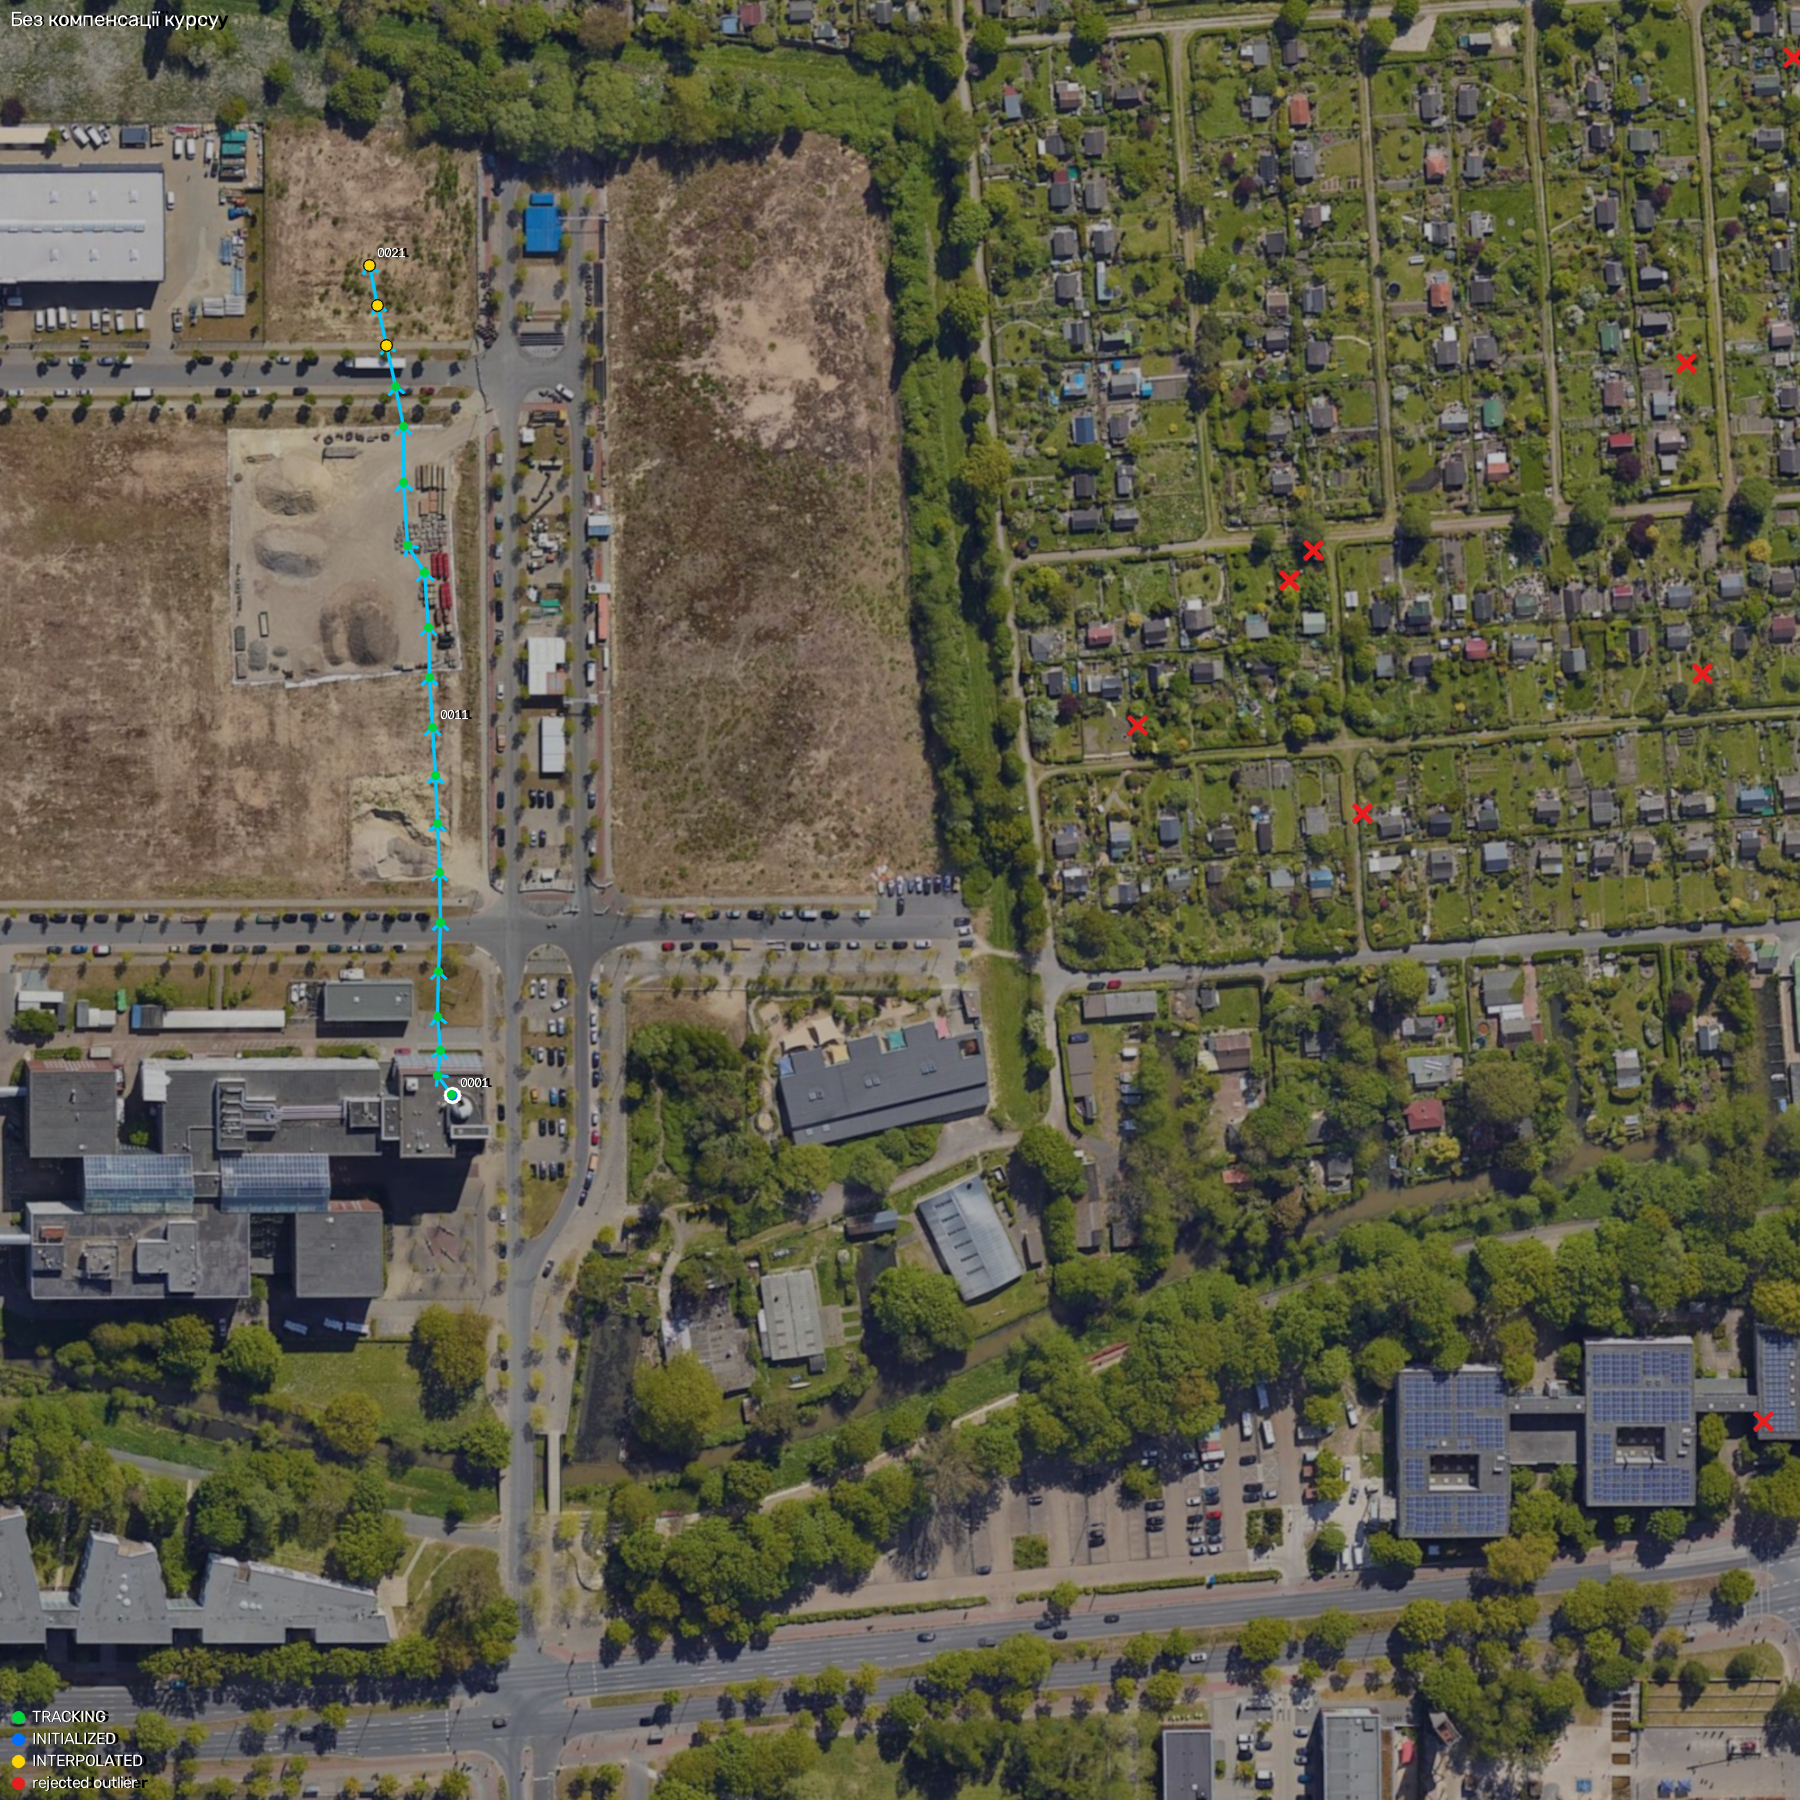
\includegraphics[width=\linewidth]{images/master/trajectory_no_yaw.png}
        \caption{без компенсації курсу}
    \end{subfigure}
    \hfill
    \begin{subfigure}{0.49\linewidth}
        \centering
        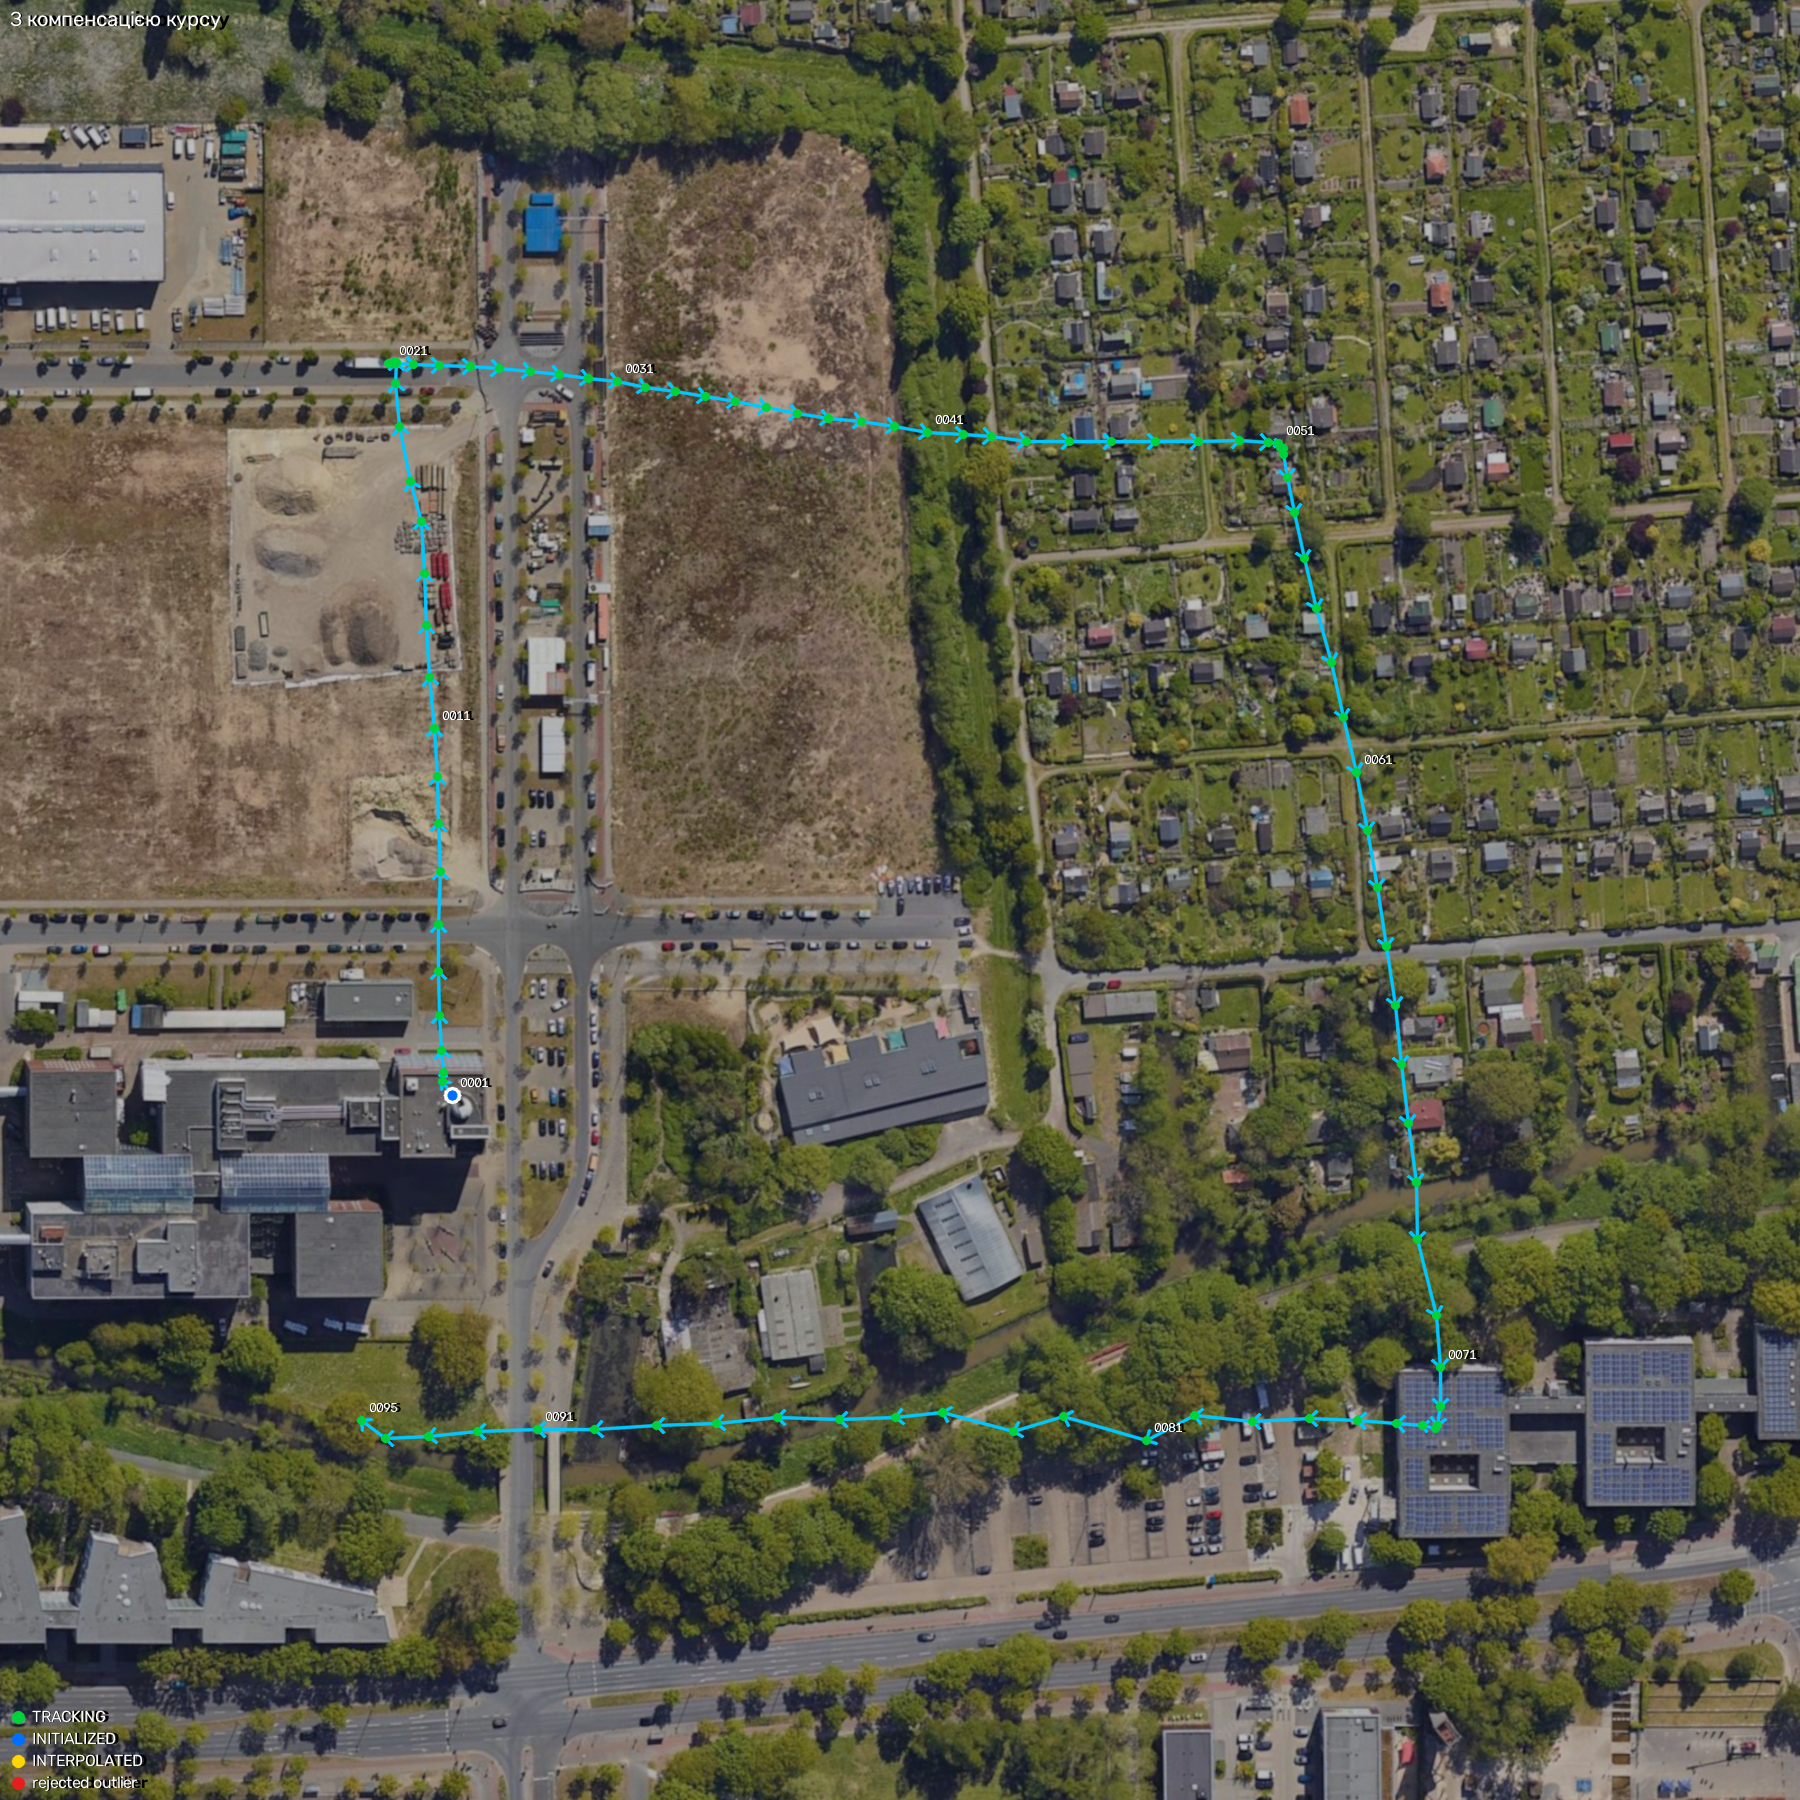
\includegraphics[width=\linewidth]{images/master/trajectory_with_yaw.png}
        \caption{з компенсацією курсу}
    \end{subfigure}
    \caption{Траєкторія, відновлена трекером: зелені точки --- \textsc{tracking}, жовті --- \textsc{interpolated}, червоні хрестики --- кандидати, відкинуті через низький бал або кінематичну перевірку}
    \label{fig:yaw}
\end{figure}

Без компенсації трекер утрачає супровід на першому розвороті (кадр 19, поворот кадру $\approx 50^\circ$). Глобальний пошук із курсом $0^\circ$ після цього вже не знаходить відповідного фрагмента. Кожен кадр у стані \textsc{lost} займає $\approx 32$~с, тому загальний час обробки зростає до 41~хв. З компенсацією всі чотири розвороти відстежено лише за прогнозом курсу; перебір додаткових гіпотез курсу знадобився для одного кадру. Компенсація курсу виявилася необхідною умовою роботи системи на реальному польоті.

\subsection{Порівняння методів LightGlue і LoFTR}
\label{sec:exp-methods}

Усі чотири конфігурації відстежили всю послідовність: 94 кадри зі статусом \textsc{tracking} і один \textsc{initialized}, лише для LightGlue + MAGSAC++ один кадр екстрапольовано. Кінематична перевірка жодного разу не відкинула оцінку, а повторна глобальна ініціалізація не знадобилася. Показники трекінгу та точності наведено в табл.~\ref{tab:tracking} і \ref{tab:accuracy}; відновлені траєкторії разом з еталоном --- на рис.~\ref{fig:traj-gt}, похибки на опорних кадрах --- на рис.~\ref{fig:error}.

\begin{table}[H]
\centering
\caption{Показники трекінгу послідовності з 95 кадрів}
\label{tab:tracking}
\small
\begin{tabular}{lcccccc}
\toprule
\multirow{2}{*}{\textbf{Конфігурація}} & \multicolumn{2}{c}{\textbf{Час кадру, с}} & \textbf{Глобальний} & \multirow{2}{*}{\textbf{Медіана} $N_{\text{in}}$} & \multirow{2}{*}{$\bar{r}$} & \multirow{2}{*}{$\bar{e}$, \px{}} \\
& середній & $P_{90}$ & \textbf{пошук, с} & & & \\
\midrule
LightGlue + RANSAC & 1,08 & 1,40 & 38,3 & 81 & 0,48 & 1,65 \\
LightGlue + MAGSAC++ & 0,78 & 1,02 & 20,1 & 87 & 0,50 & 1,73 \\
LoFTR + RANSAC & 2,72 & 2,93 & 127,9 & 316 & 0,59 & 1,27 \\
LoFTR + MAGSAC++ & 2,27 & 2,49 & 87,5 & 353 & 0,61 & 1,33 \\
\bottomrule
\end{tabular}
\end{table}

\begin{table}[H]
\centering
\caption{Похибка локалізації на 18 надійних опорних кадрах, \px{}}
\label{tab:accuracy}
\small
\begin{tabular}{lccccccc}
\toprule
\textbf{Конфігурація} & \textbf{Середня} & \textbf{Медіана} & \textbf{RMSE} & $P_{90}$ & \textbf{Макс.} & \textbf{S@10} & \textbf{S@25} \\
\midrule
LightGlue + RANSAC & 7,2 & 6,0 & 9,5 & 16,8 & 22,9 & 83\,\% & 100\,\% \\
LightGlue + MAGSAC++ & 7,5 & 5,7 & 10,2 & 16,5 & 27,5 & 78\,\% & 94\,\% \\
LoFTR + RANSAC & 4,9 & 3,1 & 7,3 & 9,0 & 24,2 & 94\,\% & 100\,\% \\
LoFTR + MAGSAC++ & 5,2 & 2,9 & 8,9 & 8,2 & 33,2 & 94\,\% & 94\,\% \\
\bottomrule
\end{tabular}
\end{table}

\begin{figure}[H]
    \centering
    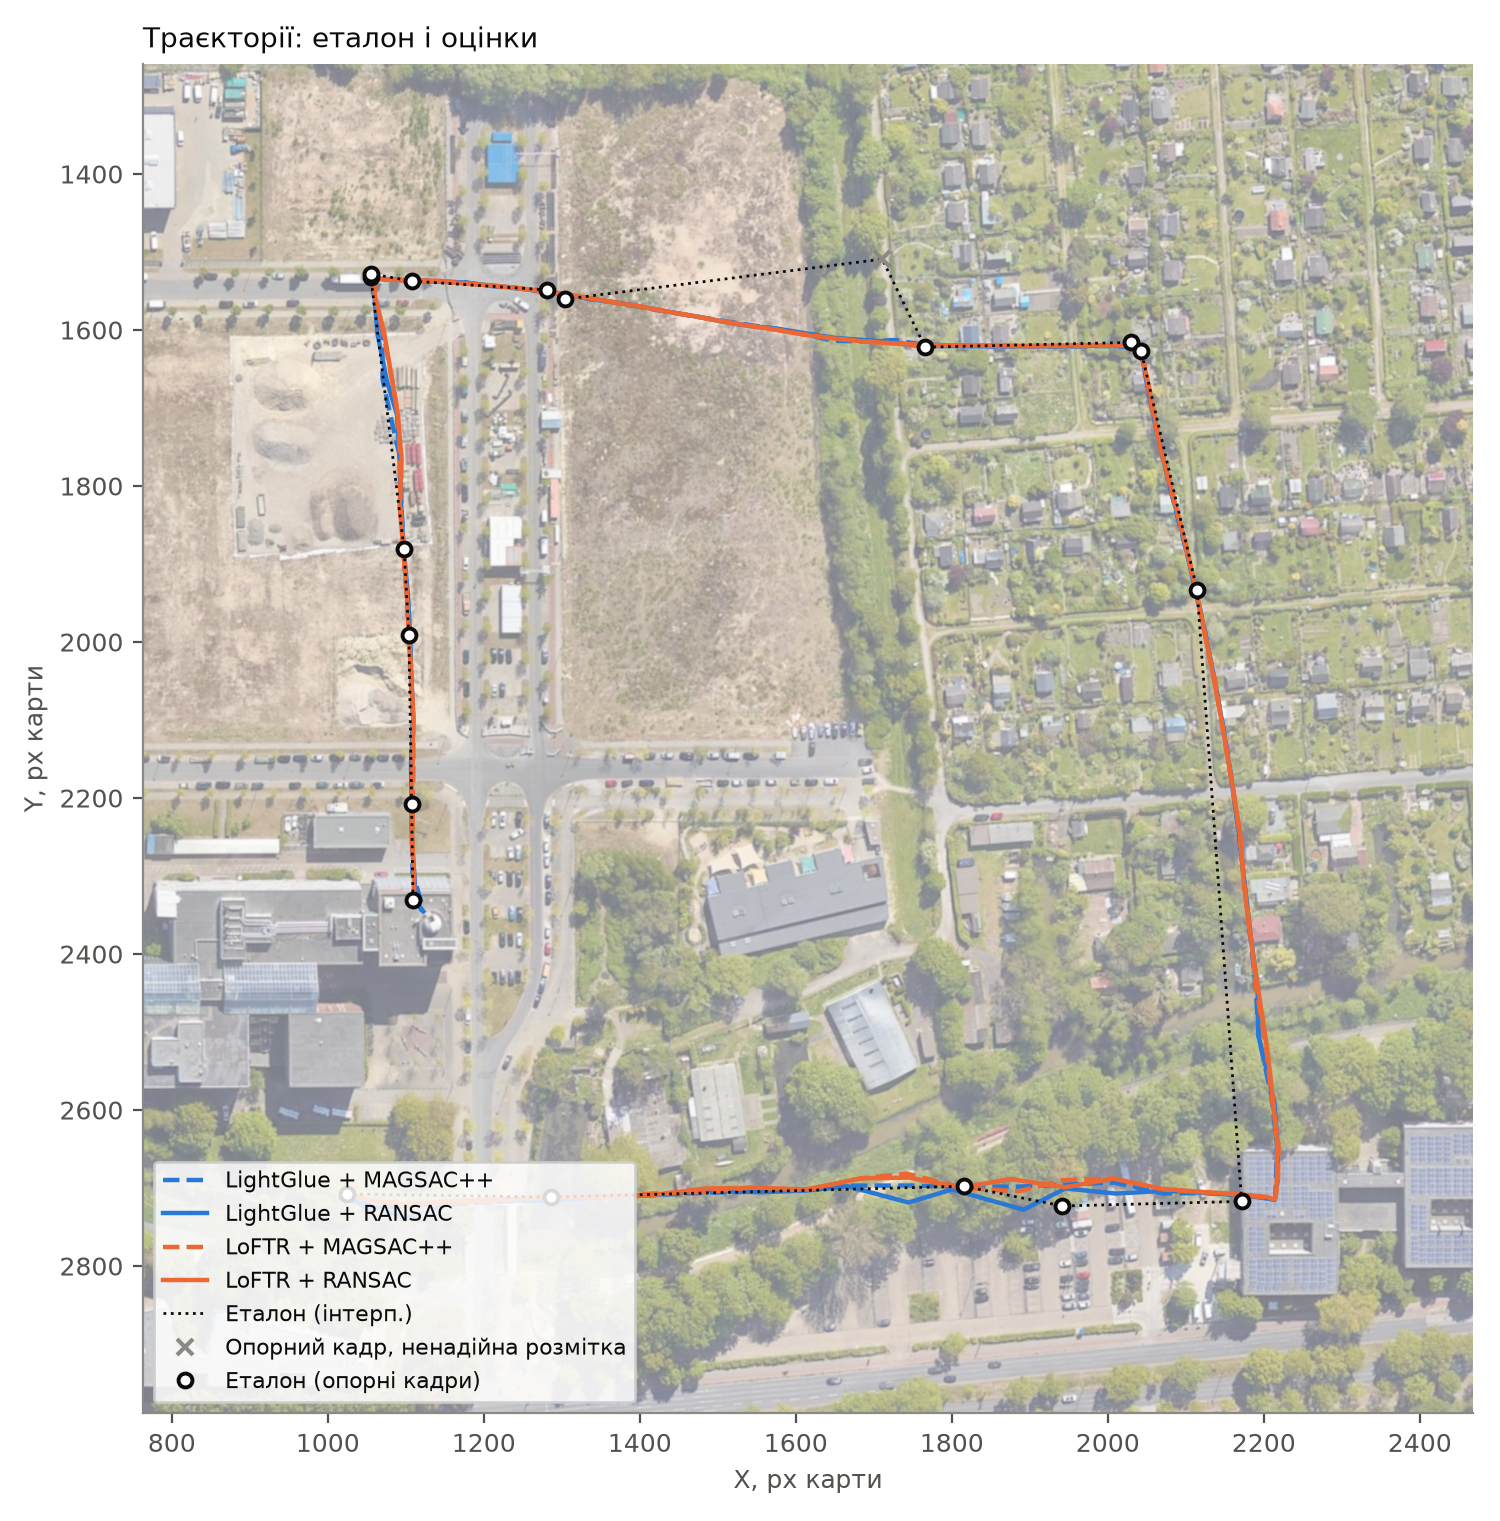
\includegraphics[width=0.8\linewidth]{images/master/trajectories_vs_gt.png}
    \caption{Траєкторії, відновлені чотирма конфігураціями, та еталонні положення опорних кадрів}
    \label{fig:traj-gt}
\end{figure}

\begin{figure}[H]
    \centering
    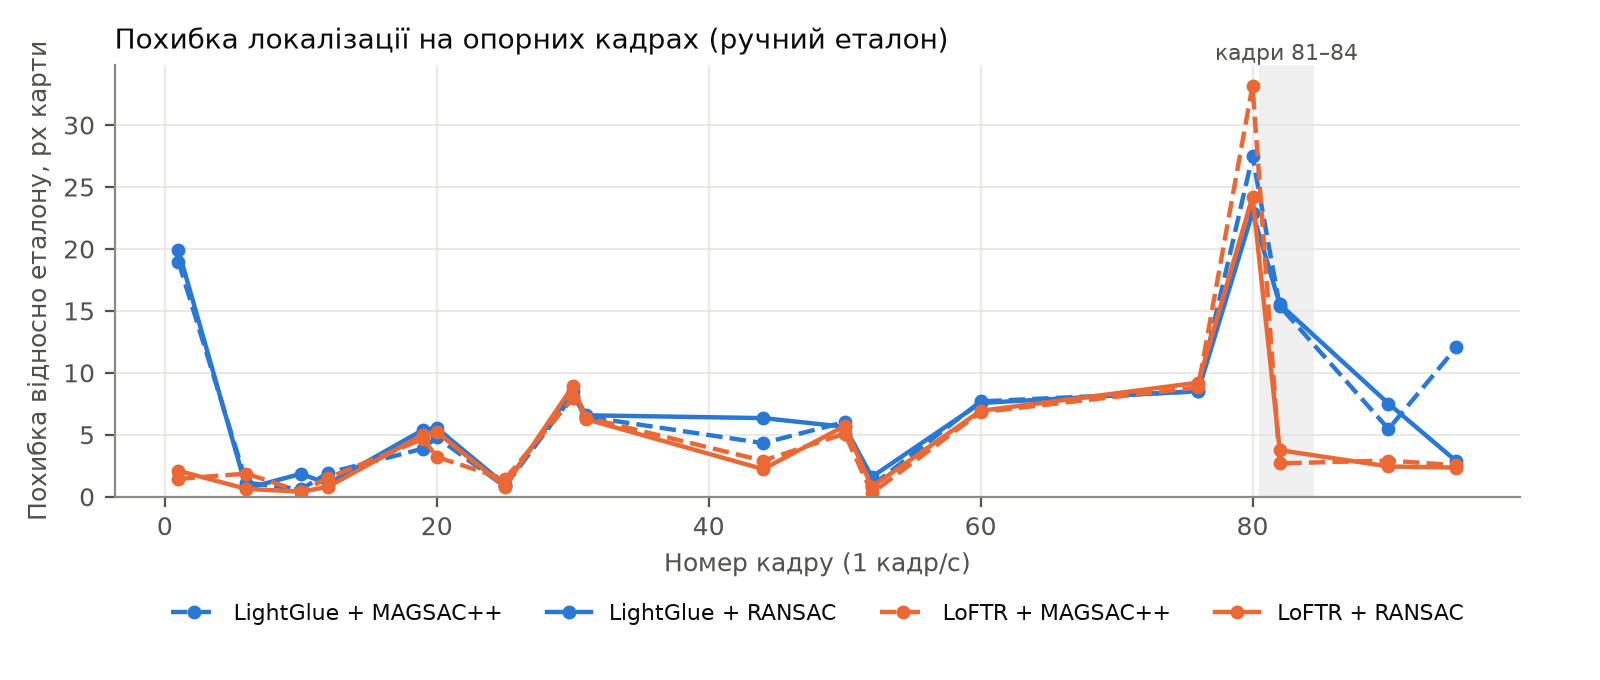
\includegraphics[width=\linewidth]{images/master/error_over_time.png}
    \caption{Похибка локалізації на опорних кадрах уздовж польоту}
    \label{fig:error}
\end{figure}

\textbf{Точність.}\\
LoFTR забезпечує меншу медіанну похибку, ніж LightGlue: $\approx 3$~\px{} проти $\approx 6$~\px{}. Частка кадрів із похибкою не більше 10~\px{} становить 94\,\% проти 78--83\,\%. У парному порівнянні з однаковим оцінювачем RANSAC LoFTR точніший на 14 з 18 опорних кадрів (знаковий тест, $p = 0{,}031$), з MAGSAC++ --- на 13 з 18 ($p = 0{,}096$). На більшості кадрів різниця між методами не перевищує 1--2~\px{}, тобто є порівнянною з невизначеністю еталона. Перевагу LoFTR формують насамперед кілька складних кадрів:
\begin{itemize}
    \item кадр 1: 19,9~\px{} у LightGlue проти 2,1~\px{} у LoFTR --- LightGlue під час ініціалізації оцінює гомографію площини даху високої будівлі (див. п.~\ref{sec:exp-pair});
    \item кадр 82 поблизу масиву дерев: 15,5~\px{} проти 3,8~\px{};
    \item кадр 90: 7,5~\px{} проти 2,4~\px{}.
\end{itemize}

На кадрі 80 усі чотири конфігурації мають близьку похибку 23--33~\px{}. Збіг похибки незалежних методів вказує на систематичну причину, спільну для всіх. Найімовірніше, це неточність еталона: усі точки розмітки цього кадру розташовані в його лівій третині (дорога й паркінг), права частина кадру зайнята деревами, а центр кадру екстрапольовано. Без кадру 80 середня похибка становить 6,2--6,3~\px{} для LightGlue і 3,6--3,7~\px{} для LoFTR; максимальна похибка LoFTR зменшується до 9,2~\px{}.

\textbf{Кількість відповідностей і швидкодія.}\\
LoFTR знаходить у 3,6--4 рази більше геометрично узгоджених відповідностей (медіана 316--353 проти 81--87) з більшою їх часткою та меншою похибкою репроєкції. Водночас LoFTR у 2,5--2,9 раза повільніший у режимі трекінгу (2,3--2,7~с проти 0,8--1,1~с на кадр) і в 3,3 (RANSAC) та 4,4 (MAGSAC++) раза повільніший під час глобального пошуку, оскільки для нього неможливе кешування ознак фрагментів. Між собою траєкторії конфігурацій відрізняються з медіаною 0,8--1,7~\px{}; найбільші розбіжності (19--43~\px{}) припадають на кадри 79--83 над деревами.

\subsection{Порівняння оцінювачів RANSAC і MAGSAC++}

Розподіл часу обробки кадру в режимі трекінгу наведено на рисунку~\ref{fig:timing}.

\begin{figure}[H]
    \centering
    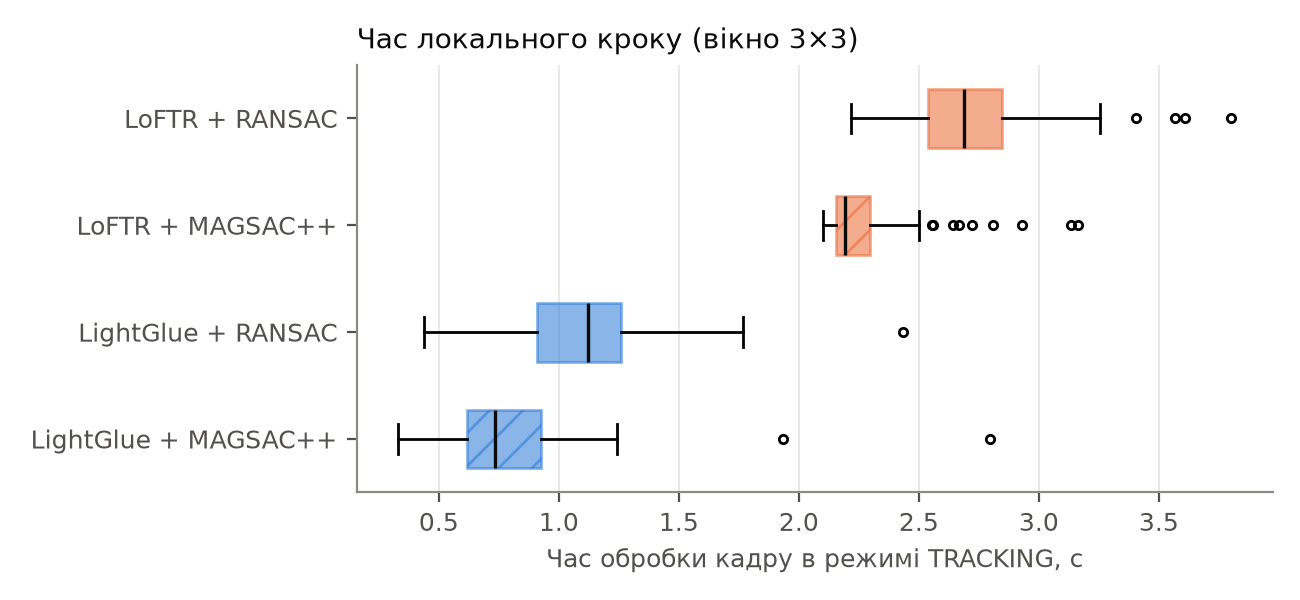
\includegraphics[width=0.75\linewidth]{images/master/timing_local.png}
    \caption{Час обробки кадру в режимі \textsc{tracking} для чотирьох конфігурацій}
    \label{fig:timing}
\end{figure}

Заміна RANSAC на MAGSAC++ скорочує час кадру на 28\,\% для LightGlue (1,08 $\to$ 0,78~с) і на 17\,\% для LoFTR (2,72 $\to$ 2,27~с), а час глобального пошуку --- у 1,9 і 1,5 раза відповідно. Виграш отримано насамперед на фрагментах, які не містять місця зйомки: на таких фрагментах реалізація RANSAC в OpenCV не може достроково зупинитися і виконує всі 5000 ітерацій, тоді як MAGSAC++ завершується за кілька мілісекунд.

Статистично значущої різниці в точності не виявлено. У парному порівнянні MAGSAC++ точніший за RANSAC на 12 з 18 кадрів для LightGlue ($p = 0{,}24$) і на 9 з 18 для LoFTR ($p = 1{,}0$), медіанна різниця не перевищує 0,2~\px{}. Траєкторії, отримані з різними оцінювачами, відрізняються з медіаною 1,2~\px{} (LightGlue) і 0,8~\px{} (LoFTR). Таким чином, MAGSAC++ дає змогу пришвидшити систему без втрати точності. Конфігурація LightGlue + MAGSAC++ --- єдина, що забезпечує обробку кадру не довше 1~с (середнє 0,78~с, $P_{90}$ 1,02~с).

\subsection{Стійкість до спотворень зображення}
\label{sec:exp-robust}

Для 19 кадрів (кожен п'ятий кадр послідовності) штучно застосовано спотворення до оригінального кадру $1920 \times 1080$:
\begin{itemize}
    \item зниження яскравості $I' = \alpha I$;
    \item зниження контрасту $I' = \alpha (I - \mu) + \mu$, де $\mu$ --- середнє значення каналу;
    \item адитивний гауссів шум;
    \item лінійне розмиття руху;
    \item поворот кадру без компенсації;
    \item помилка у заданому масштабі $s_f$.
\end{itemize}
Пул фрагментів і компенсація курсу були такими самими, як у трекері на відповідному кадрі. Для кожного кадру обчислено відношення $N_{\text{in}}$ до значення для неспотвореного кадру та зміщення знайденого центру. Результати наведено в табл.~\ref{tab:robust} і на рис.~\ref{fig:robust}.

\begin{table}[H]
\centering
\caption{Стійкість до спотворень (19 кадрів): частка локалізованих кадрів і медіанне відношення $N_{\text{in}} / N_{\text{in}}^{\text{без спотв.}}$}
\label{tab:robust}
\small
\begin{tabular}{lcccc}
\toprule
\multirow{2}{*}{\textbf{Спотворення}} & \multicolumn{2}{c}{\textbf{LightGlue}} & \multicolumn{2}{c}{\textbf{LoFTR}} \\
\cmidrule(lr){2-3}\cmidrule(lr){4-5}
& локалізовано & відношення & локалізовано & відношення \\
\midrule
яскравість $\alpha = 0{,}7$ / $0{,}5$ & 100 / 100\,\% & 1,00 / 1,01 & 100 / 100\,\% & 0,97 / 0,97 \\
контраст $\alpha = 0{,}7$ / $0{,}5$ & 100 / 100\,\% & 1,02 / 0,99 & 100 / 100\,\% & 1,00 / 0,97 \\
шум $\sigma = 10$ / $25$ & 95 / 95\,\% & 0,99 / 0,92 & 100 / 95\,\% & 1,02 / 0,95 \\
розмиття 5 / 9 пікселів & 100 / 100\,\% & 1,02 / 1,02 & 100 / 100\,\% & 1,02 / 1,04 \\
поворот $15^\circ$ / $30^\circ$ & 95 / 95\,\% & 1,03 / 0,99 & 95 / 95\,\% & 0,82 / 0,52 \\
поворот $45^\circ$ & 53\,\% & 0,35 & 11\,\% & 0 \\
поворот $90^\circ$ & 0\,\% & 0 & 0\,\% & 0 \\
масштаб $\times 0{,}8$ / $\times 1{,}25$ & 100 / 95\,\% & 0,68 / 1,29 & 100 / 100\,\% & 0,71 / 1,05 \\
\bottomrule
\end{tabular}
\end{table}

\begin{figure}[H]
    \centering
    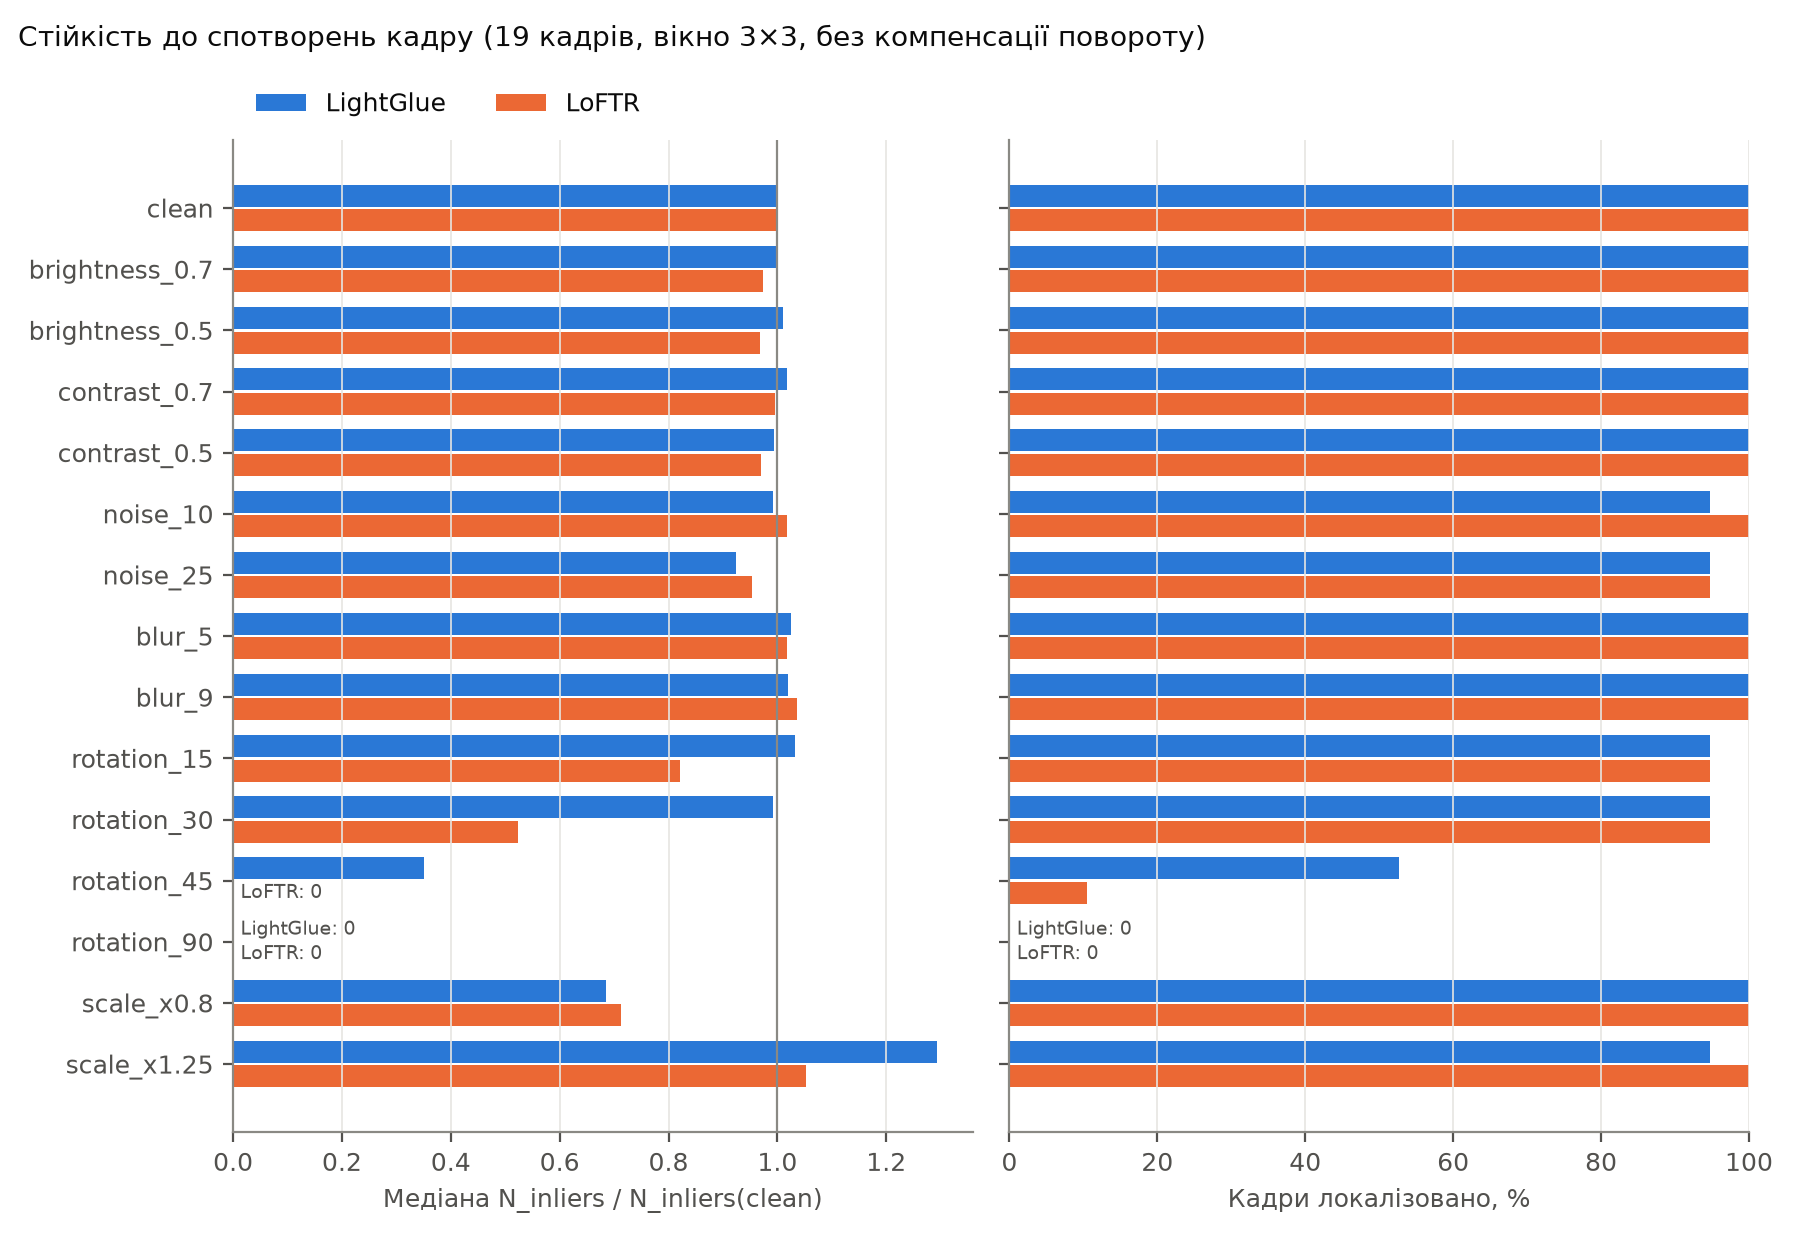
\includegraphics[width=\linewidth]{images/master/robustness.png}
    \caption{Стійкість методів до спотворень кадру}
    \label{fig:robust}
\end{figure}

Зміни яскравості й контрасту, гауссів шум і розмиття в досліджених межах практично не впливають на результат: кількість геометрично узгоджених відповідностей зберігається, а медіанне зміщення центру не перевищує 1,5~\px{}. Слабкий вплив розмиття частково пояснюється тим, що після масштабування кадру з коефіцієнтом 0,27 ядро 9 пікселів зменшується до $\approx 2{,}4$ пікселя.

Визначальним чинником виявився поворот кадру. LightGlue зберігає працездатність до $30^\circ$, а LoFTR втрачає половину відповідностей уже при $30^\circ$. При $45^\circ$ локалізовано лише 53\,\% (LightGlue) і 11\,\% (LoFTR) кадрів, при $90^\circ$ --- жодного. Ці результати кількісно обґрунтовують компенсацію курсу, описану в п.~\ref{sec:tracking}. Похибка масштабу на 20--25\,\% не призводить до втрати локалізації, але зменшення заданого масштабу на 20\,\% скорочує кількість відповідностей приблизно на 30\,\%.

\subsection{Аналіз проблемних ділянок місцевості}

Для кожного кадру за контуром огляду обчислено дві ознаки ділянки ортофотоплану:
\begin{itemize}
    \item частку рослинності за індексом Excess Green $\text{ExG} = 2g - r - b$ у хроматичних координатах \cite{exg} (піксель вважається рослинністю, якщо $\text{ExG} > 0{,}05$);
    \item текстурованість --- середній модуль градієнта Собеля яскравості.
\end{itemize}
Залежність кількості геометрично узгоджених відповідностей від номера кадру та частки рослинності наведено на рисунку~\ref{fig:terrain}, кореляції --- у табл.~\ref{tab:terrain}.

\begin{figure}[H]
    \centering
    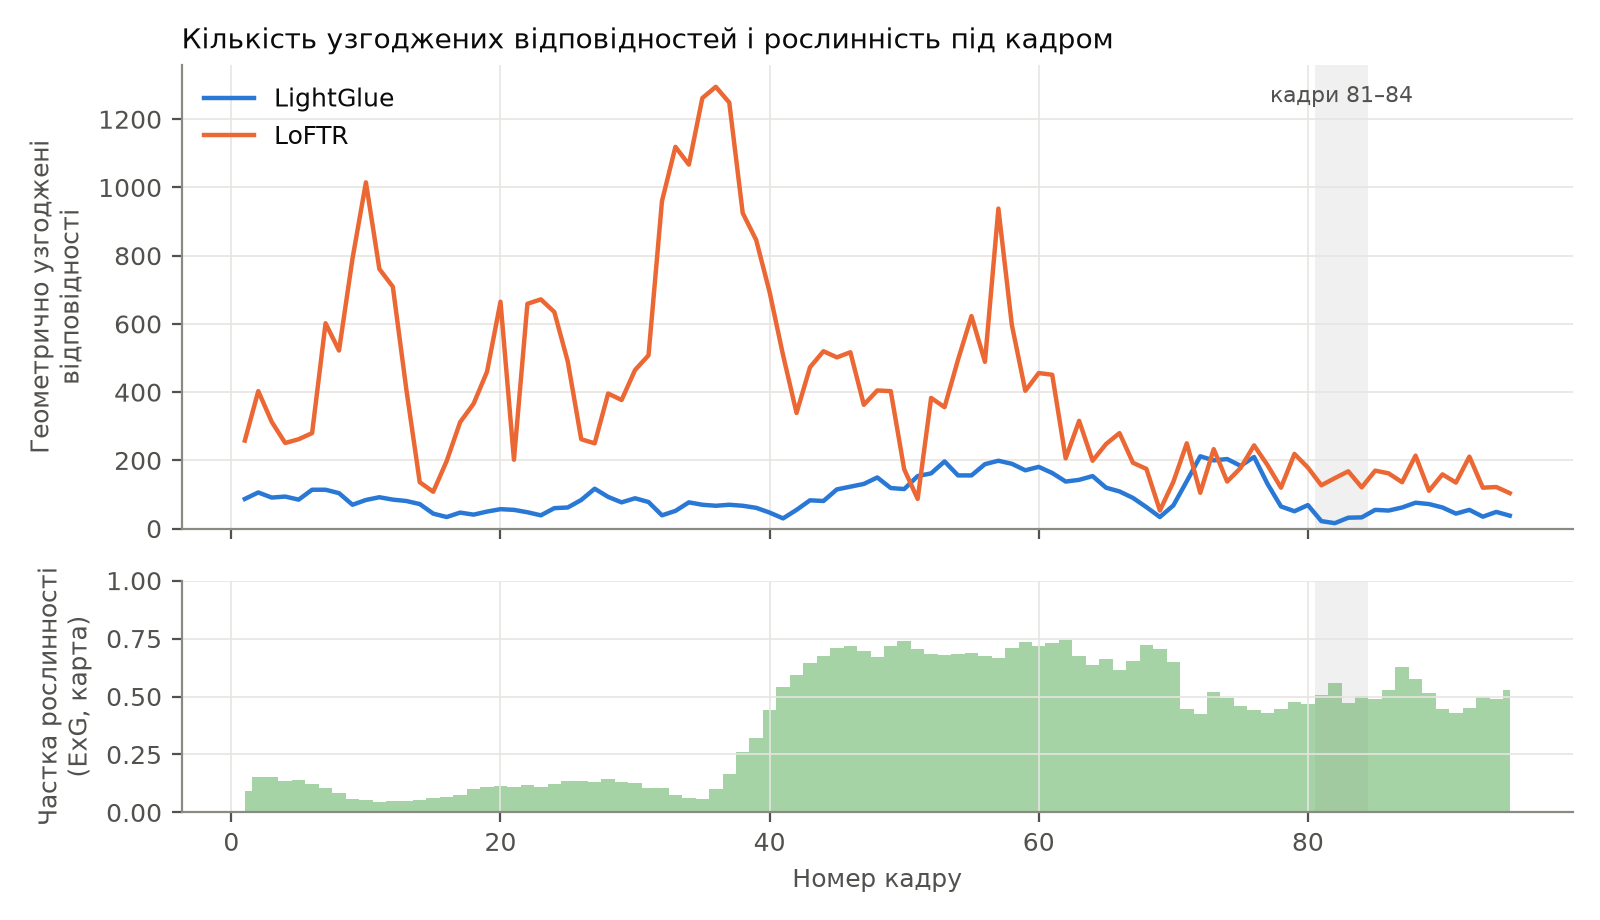
\includegraphics[width=\linewidth]{images/master/inliers_vs_terrain.png}
    \caption{Кількість геометрично узгоджених відповідностей уздовж польоту (вгорі) і частка рослинності під кадром (внизу); сірим виділено кадри 81--84}
    \label{fig:terrain}
\end{figure}

\begin{table}[H]
\centering
\caption{Зв'язок кількості геометрично узгоджених відповідностей з ознаками місцевості (кореляція Спірмена $\rho$, RANSAC)}
\label{tab:terrain}
\begin{tabular}{lcccc}
\toprule
\textbf{Метод} & $\rho$ (рослинність) & $\rho$ (текстура) & \textbf{Медіана} $N_{\text{in}}$, кадри 81--84 & \textbf{Медіана} $N_{\text{in}}$, усі \\
\midrule
LightGlue & $+0{,}37$ & $+0{,}65$ & 27 & 81 \\
LoFTR & $-0{,}29$ & $+0{,}29$ & 138 & 316 \\
\bottomrule
\end{tabular}
\end{table}

На ділянці кадрів 81--84 (паркінг і канал, оточені деревами) кількість геометрично узгоджених відповідностей падає втричі для LightGlue і вдвічі для LoFTR. Саме тут методи найбільше розходяться між собою. Водночас частка рослинності під кадром сама по собі не пояснює це падіння: для LightGlue кореляція з нею навіть додатна, оскільки дачні ділянки з будівлями мають високу частку рослинності, але багаті на деталі. Кращим предиктором для LightGlue є текстурованість ($\rho = 0{,}65$); для LoFTR зв'язок з обома ознаками слабкий. Імовірною причиною падіння на кадрах 81--84 є сезонна різниця крон листяних дерев (на відео --- без листя, на карті --- з листям), однак підтвердження цієї гіпотези потребує окремого дослідження.

% TODO: експерименти з розміром фрагмента (256/512/768/1024) і часткою перекриття (25/50 %),
%       передбачені технічним завданням, ще не проведено. Після їх виконання додати
%       підрозділ з результатами (див. обмеження нижче щодо розміру фрагмента 512).

\subsection{Обмеження розробленої системи}

Під час експериментів виявлено такі обмеження:
\begin{itemize}
    \item \textbf{Плоска модель сцени.} Гомографія описує лише площину. Високі будівлі спричиняють паралакс, і RANSAC може оцінити площину даху замість площини землі (кадр 1 у LightGlue, кадр 2 у LoFTR).
    \item \textbf{Розмір фрагмента.} Контур огляду кадру ($\approx 518 \times 292$~\px{}) ширший за фрагмент 512~\px{}, тому жоден фрагмент не містить кадр повністю.
    \item \textbf{Фіксований масштаб.} Масштаб кадру $s_f$ відкалібровано на одному кадрі, і він вважається сталим. Під час польоту оцінений масштаб гомографії змінювався в межах 0,20--0,32 (медіана 0,269), проте в трекері він не уточнюється.
    \item \textbf{Чутливість до повороту.} Без компенсації курсу обидва методи непрацездатні при повороті кадру на $45^\circ$ і більше; перший глобальний пошук виконується з курсом $0^\circ$.
    \item \textbf{Швидкодія.} Повний перебір карти займає 20--128~с залежно від конфігурації. Обмеження 1~с на кадр у режимі трекінгу на використаному GPU виконує лише LightGlue + MAGSAC++.
    \item \textbf{Одиниці вимірювання.} Без просторової прив'язки ортофотоплану похибки визначено в пікселях карти; переведення в метри потребує відомого розміру пікселя.
    \item \textbf{Обсяг даних і еталона.} Дослідження виконано на одному польоті (95 кадрів) і 18 опорних кадрах. Опорні кадри обрано за наявністю наземних орієнтирів, тому міські ділянки в еталоні представлені ширше, ніж у польоті загалом.
\end{itemize}

\subsection{Висновки за результатами експериментів}

\begin{enumerate}
    \item Розроблена система автоматично знаходить відповідний фрагмент ортофотоплану для кадру БпЛА без апріорної інформації про місце зйомки та відновлює траєкторію польоту. На послідовності з 95 кадрів усі чотири конфігурації локалізували кожен кадр без втрати супроводу.
    \item Медіанна похибка локалізації на опорних кадрах становить $\approx 3$~\px{} для LoFTR і $\approx 6$~\px{} для LightGlue; не більше ніж 10~\px{} помиляється 94\,\% і 78--83\,\% кадрів відповідно. LoFTR точніший на більшості кадрів, і його перевага найпомітніша на складних ділянках (дах високої будівлі, дерева).
    \item LightGlue у 2,5--2,9 раза швидший за LoFTR у режимі трекінгу і допускає кешування ознак карти. Конфігурація LightGlue + MAGSAC++ --- єдина, що обробляє кадр не довше 1~с (0,78~с у середньому).
    \item MAGSAC++ скорочує час обробки на 17--28\,\% без статистично значущої зміни точності, тому його доцільно використовувати замість класичного RANSAC.
    \item Обидва методи стійкі до змін яскравості, контрасту, шуму та помірного розмиття, але не до повороту кадру понад $30$--$45^\circ$. Компенсація курсу за оцінкою кута з гомографії попередніх кадрів виявилася необхідною: без неї супровід утрачається на першому розвороті.
    \item Результати курсової роботи щодо переваги LightGlue за кількістю відповідностей отримано за нерівних умов (різний масштаб вхідних зображень). За однакових умов LoFTR знаходить більше геометрично узгоджених відповідностей.
    \item Вибір методу визначається вимогами застосування: LoFTR --- для вищої точності, LightGlue + MAGSAC++ --- для обробки в реальному часі на обмеженому обладнанні.
\end{enumerate}

% =============================================================================
\providecommand{\px}{пкс}
\providecommand{\code}[1]{\texttt{#1}}

\newpage
\section{Результати експериментів та їх оцінка}
\label{sec:experiments}

\subsection{Методика експериментального дослідження}

\textbf{Дані та обладнання.}\\
Усі експерименти виконано на даних, описаних у розділі~\ref{sec:implementation}: ортофотоплан $6200 \times 4320$~пікселів, розбитий на 384 фрагменти $512 \times 512$ з перекриттям 50\,\%, і 95 кадрів відео польоту БпЛА з частотою 1~кадр/с. Обчислення виконано на GPU NVIDIA GeForce GTX 1650. Якщо не зазначено інше, використано параметри за замовчуванням: $s_f = 0{,}27$, $k = 1$, поріг RANSAC 3~\px{}, мінімум 15 геометрично узгоджених відповідностей.

\textbf{Досліджувані конфігурації.}\\
Порівнювалися чотири конфігурації системи --- поєднання методу зіставлення (LightGlue або LoFTR) та оцінювача гомографії (RANSAC або MAGSAC++). Решта етапів (масштабування, геометрична перевірка, фільтр і ранжування, трекер, компенсація курсу) для всіх конфігурацій однакові. Це забезпечує коректність порівняння: на відміну від курсової роботи, обидва методи отримують зображення однакового масштабу.

\textbf{Метрики зіставлення.}\\
Для пари <<кадр --- фрагмент>> використовуються:
\begin{itemize}
    \item $N_{\text{all}}$ --- кількість відповідностей, які повернув метод;
    \item $N_{\text{in}}$ --- кількість геометрично узгоджених відповідностей (похибка репроєкції не більша за поріг RANSAC);
    \item $r = N_{\text{in}} / N_{\text{all}}$ --- частка геометрично узгоджених відповідностей;
    \item $\bar{e}$ --- середня похибка репроєкції геометрично узгоджених відповідностей, \px{}. За побудовою вона не перевищує порогу RANSAC, тому характеризує точність відповідностей, а не успішність локалізації;
    \item час обробки, с.
\end{itemize}

\textbf{Метрики локалізації.}\\
Похибка локалізації кадру $i$ визначається відносно еталонного положення (п.~\ref{sec:gt}):
\begin{equation}
E_i = \sqrt{(X_i - X_i^{\text{ет}})^2 + (Y_i - Y_i^{\text{ет}})^2}, \quad \text{\px{}}.
\end{equation}
За сукупністю кадрів обчислюються середня, медіанна та максимальна похибка, середньоквадратична похибка $\text{RMSE} = \sqrt{\tfrac{1}{N}\sum_i E_i^2}$, 90-й процентиль $P_{90}$, а також частка успішних локалізацій
\begin{equation}
\text{Success@}K = \frac{\left|\{ i : E_i \le K \}\right|}{N}, \qquad K \in \{10, 25, 50\}~\text{\px{}},
\end{equation}
де $N$ --- кількість усіх кадрів з еталоном; кадри, для яких система не видала положення, вважаються неуспішними. Ортофотоплан не має просторової прив'язки, тому похибки наведено в пікселях карти і в метри не переводяться.

\subsection{Еталонні координати}
\label{sec:gt}

Для обчислення похибки локалізації потрібне еталонне положення кадру, незалежне від системи, що оцінюється. Використання як еталона результатів самої системи або їхнього візуального <<уточнення>> призвело б до заниженої оцінки похибки, тому еталон побудовано за ручними відповідностями точок.

\textbf{Процедура розмітки.}\\
Для опорного кадру оператор у спеціально розробленому інструменті вказує щонайменше 5 пар відповідних точок <<кадр $\leftrightarrow$ карта>>, розташованих на рівні землі (кути дорожньої розмітки та бордюрів, перехрестя доріжок, основи стовпів). Дахи будівель не використовуються, оскільки через паралакс вони зміщені відносно земної поверхні. За всіма парами методом найменших квадратів (без RANSAC) оцінюється гомографія $H_{\text{ет}}$, і центр кадру переноситься на карту. Приклад розмітки наведено на рисунку~\ref{fig:gt-example}.

\begin{figure}[H]
    \centering
    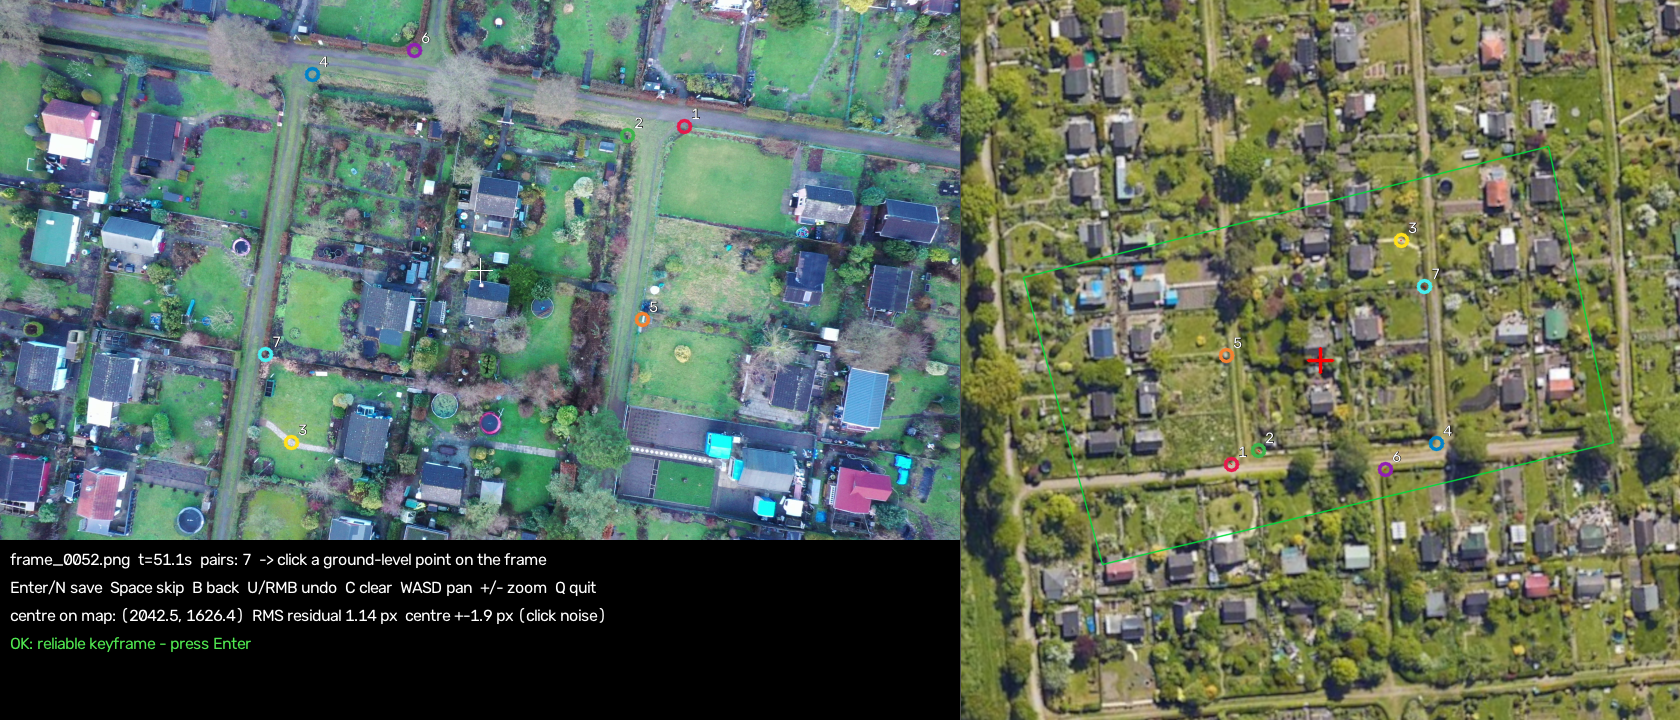
\includegraphics[width=\linewidth]{images/master/gt_annotation_example.png}
    \caption{Розмітка еталонного положення кадру 52 (кадр повернутий на $\approx 170^\circ$ відносно карти): пари точок пронумеровано, зеленим --- спроєктований контур кадру, червоним хрестиком --- центр кадру}
    \label{fig:gt-example}
\end{figure}

\textbf{Контроль якості розмітки.}\\
З чотирьох пар гомографія визначається точно, тому залишкова похибка дорівнює нулю й не дає змоги виявити помилку оператора. У першій версії розмітки саме такі кадри (по 4 пари, скупчені в одній частині кадру) давали <<похибку>> системи понад 100~\px{} для всіх методів одночасно. Тому опорний кадр вважається надійним, якщо:
\begin{enumerate}
    \item вказано не менше 5 пар;
    \item залишкова похибка кожної пари не перевищує 3~\px{}, інакше одна з точок хибна;
    \item 95-й процентиль зміщення центру за випадкового шуму кліків ($\sigma = 2$~пікселі кадру та 1~піксель карти, метод Монте-Карло) не перевищує 5~\px{}, інакше точки скупчені або центр кадру розташований далеко від них.
\end{enumerate}
Критерій не використовує результатів системи. Опорні кадри обрано візуально так, щоб на них були чіткі наземні орієнтири і щоб вони рівномірно покривали політ, включно з розворотами. Кадри над пустирем (33--40) і каналом (66--69) пропущено через відсутність надійних точок.

Розмічено 19 опорних кадрів, з них 18 надійних: 5--8 пар на кадр (у середньому 6,2), медіанна невизначеність центру 2,6~\px{} (максимум 5,0~\px{}), найбільша залишкова похибка пари --- 3,0~\px{}. Ненадійний кадр 40 (пустир, 4 пари) в метрики не включено. Для 7 надійних кадрів центр кадру лежить поза областю вказаних точок, тобто його положення екстрапольовано. Шум кліків цим критерієм враховано, але систематичні похибки (дисторсія ширококутного об'єктива, паралакс) за межами точок не оцінюються, що слід мати на увазі під час аналізу окремих кадрів.

Для кадрів між опорними еталон можна лінійно інтерполювати в часі, однак на розворотах інтерполяція <<зрізає>> траєкторію. Через це похибка за інтерпольованим еталоном вимірює насамперед похибку інтерполяції: для всіх чотирьох конфігурацій вона однакова, $\approx 38$~\px{}. Тому всі наведені нижче похибки обчислено лише за 18 надійними опорними кадрами.

\subsection{Зіставлення кадру з відомим фрагментом карти}
\label{sec:exp-pair}

\textbf{Результати для еталонної пари.}\\
Для перевірки конвеєра використано пару з курсової роботи: кадр 2 і фрагмент карти, що містить місце зйомки (результати --- у табл.~\ref{tab:pair}, приклади відповідностей --- на рис.~\ref{fig:pair}).

\begin{table}[H]
\centering
\caption{Зіставлення еталонної пари <<кадр 2 --- фрагмент 196>> (GPU, медіана часу з 5 запусків)}
\label{tab:pair}
\begin{tabular}{lcccccc}
\toprule
\textbf{Метод} & $N_{\text{all}}$ & $N_{\text{in}}$ & $r$ & $\bar{e}$, \px{} & масштаб $\sigma$ & час, с \\
\midrule
LightGlue & 310 & 89 & 0,29 & 1,58 & 0,267 & 0,25 \\
LoFTR & 631 & 184 & 0,29 & 1,40 & 0,202 & 0,27 \\
\bottomrule
\end{tabular}
\end{table}

\begin{figure}[H]
    \centering
    \begin{subfigure}{\linewidth}
        \centering
        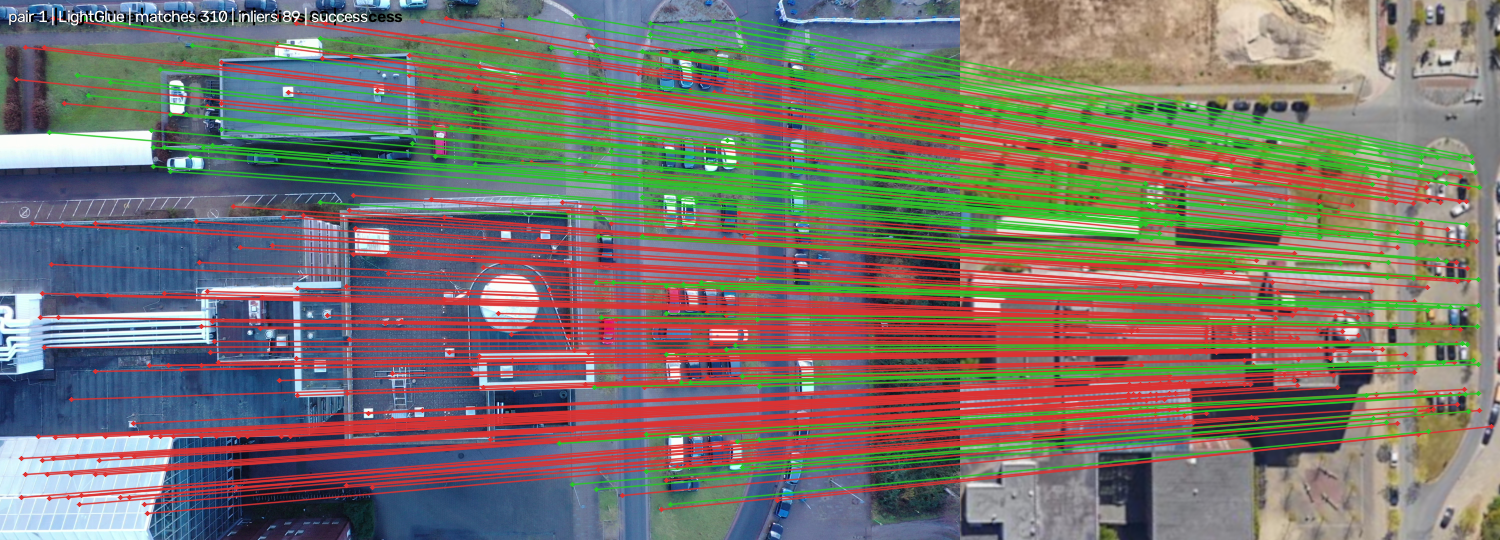
\includegraphics[width=0.92\linewidth]{images/master/pair_lightglue_matches.png}
        \caption{LightGlue}
    \end{subfigure}
    \vspace{2mm}
    \begin{subfigure}{\linewidth}
        \centering
        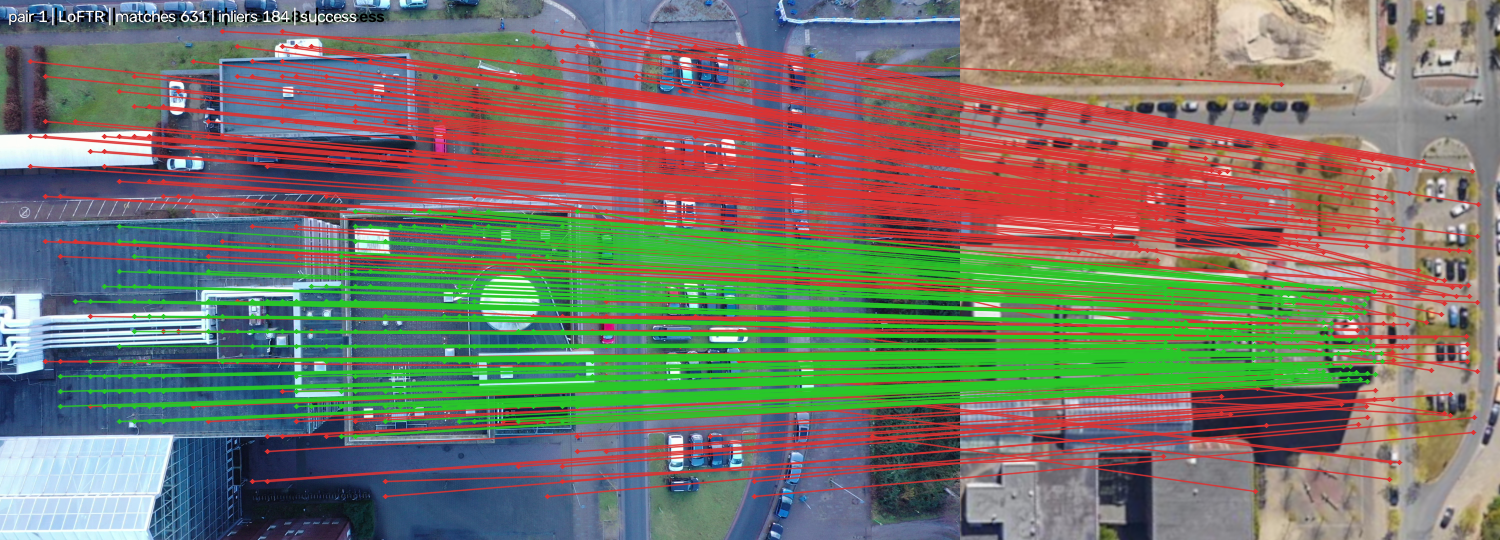
\includegraphics[width=0.92\linewidth]{images/master/pair_loftr_matches.png}
        \caption{LoFTR}
    \end{subfigure}
    \caption{Відповідності між кадром 2 (ліворуч) і фрагментом карти (праворуч): зеленим --- геометрично узгоджені, червоним --- відкинуті RANSAC}
    \label{fig:pair}
\end{figure}

\textbf{Виправлення методики курсової роботи.}\\
У курсовій роботі на цій парі LightGlue мав 229 геометрично узгоджених відповідностей проти 117 у LoFTR і працював повільніше (6,55~с проти 4,18~с). Аналіз прототипу показав, що ці результати отримано за нерівних умов. По-перше, SuperPoint неявно масштабував вхідні зображення до 1024~пікселів, тоді як LoFTR працював із 512. По-друге, обидва методи бачили лише центральну квадратну частину кадру, без нормалізації масштабу. По-третє, час вимірювався без прогрівання моделей. За однакових умов (табл.~\ref{tab:pair}) співвідношення змінюється: LoFTR знаходить удвічі більше геометрично узгоджених відповідностей за однакової їх частки, а час обробки пари на GPU для обох методів становить $\approx 0{,}25$~с. Тому числові результати курсової роботи надалі не використовуються.

\textbf{Калібрування масштабу кадру.}\\
Початкову оцінку $s_f \approx 0{,}25$ отримано вручну. Для її уточнення кадр 2 зіставлено з фрагментом карти $1024 \times 1024$, що повністю містить контур кадру. Обидва методи за обох оцінювачів і робочих масштабів $k \in \{1;\, 1{,}5\}$ дали узгоджений масштаб гомографії $\sigma = 0{,}267$--$0{,}277$, а оцінки центра кадру розійшлися не більше ніж на 16~\px{}. Отже, прийнято $s_f = 0{,}27$: кадр $1920 \times 1080$ покриває на карті ділянку $\approx 518 \times 292$~\px{}, ширшу за фрагмент 512~\px{}.

\textbf{Вплив непланарності сцени.}\\
На фрагменті 196 масштаб гомографії LoFTR ($\sigma = 0{,}20$) суттєво менший за калібрувальний (табл.~\ref{tab:pair}). Геометрично узгоджені відповідності LoFTR зосереджені на даху високої будівлі, ближчому до камери, ніж земля, тому RANSAC оцінює гомографію площини даху, а не площини землі (рис.~\ref{fig:pair}б). Центр кадру при цьому все одно визначається з похибкою $\approx 15$~\px{}, оскільки він сам розташований на цьому даху. Цей ефект є прямим наслідком припущення про плоску сцену.

\textbf{Контрольна перевірка на хибних фрагментах.}\\
Кадр 2 зіставлено з 33 фрагментами, серед яких є як сусідні до місця зйомки, так і віддалені. Фрагменти, що не перетинаються з кадром, дали щонайбільше 15 (LightGlue) і 14 (LoFTR) геометрично узгоджених відповідностей і всі були відкинуті: частина за порогом $N_{\text{in}} \ge 15$, частина --- перевіркою правдоподібності гомографії. Усі фрагменти, що перетинаються з кадром, дали від 18 до 240 таких відповідностей і пройшли перевірку. Запас між цими групами невеликий, тому для вибору фрагмента додатково використовуються частка відповідностей і умова потрапляння центра кадру у фрагмент (п.~\ref{sec:search}).

\subsection{Автоматичний пошук фрагмента для одиночного кадру}

Для кадру 2 виконано пошук без будь-якої інформації про місце зйомки (табл.~\ref{tab:search}, рис.~\ref{fig:global-loc}).

\begin{table}[H]
\centering
\caption{Автоматичний пошук фрагмента для кадру 2}
\label{tab:search}
\small
\begin{tabular}{lccccc}
\toprule
\textbf{Запуск} & \textbf{Перевірено} & \textbf{Пройшли фільтр} & \textbf{Переможець} & \textbf{Центр $(X, Y)$, \px{}} & \textbf{Час, с} \\
\midrule
LightGlue, уся карта, кеш & 384 & 5 & 220 & (1121,4;\ 2344,7) & 33 \\
LoFTR, обмежена область & 56 & 5 & 197 & (1108,6;\ 2327,5) & 18 \\
LoFTR, кожен 2-й рядок і стовпець & 96 & 1 & 197 & (1108,6;\ 2327,5) & 32 \\
\bottomrule
\end{tabular}
\end{table}

\begin{figure}[H]
    \centering
    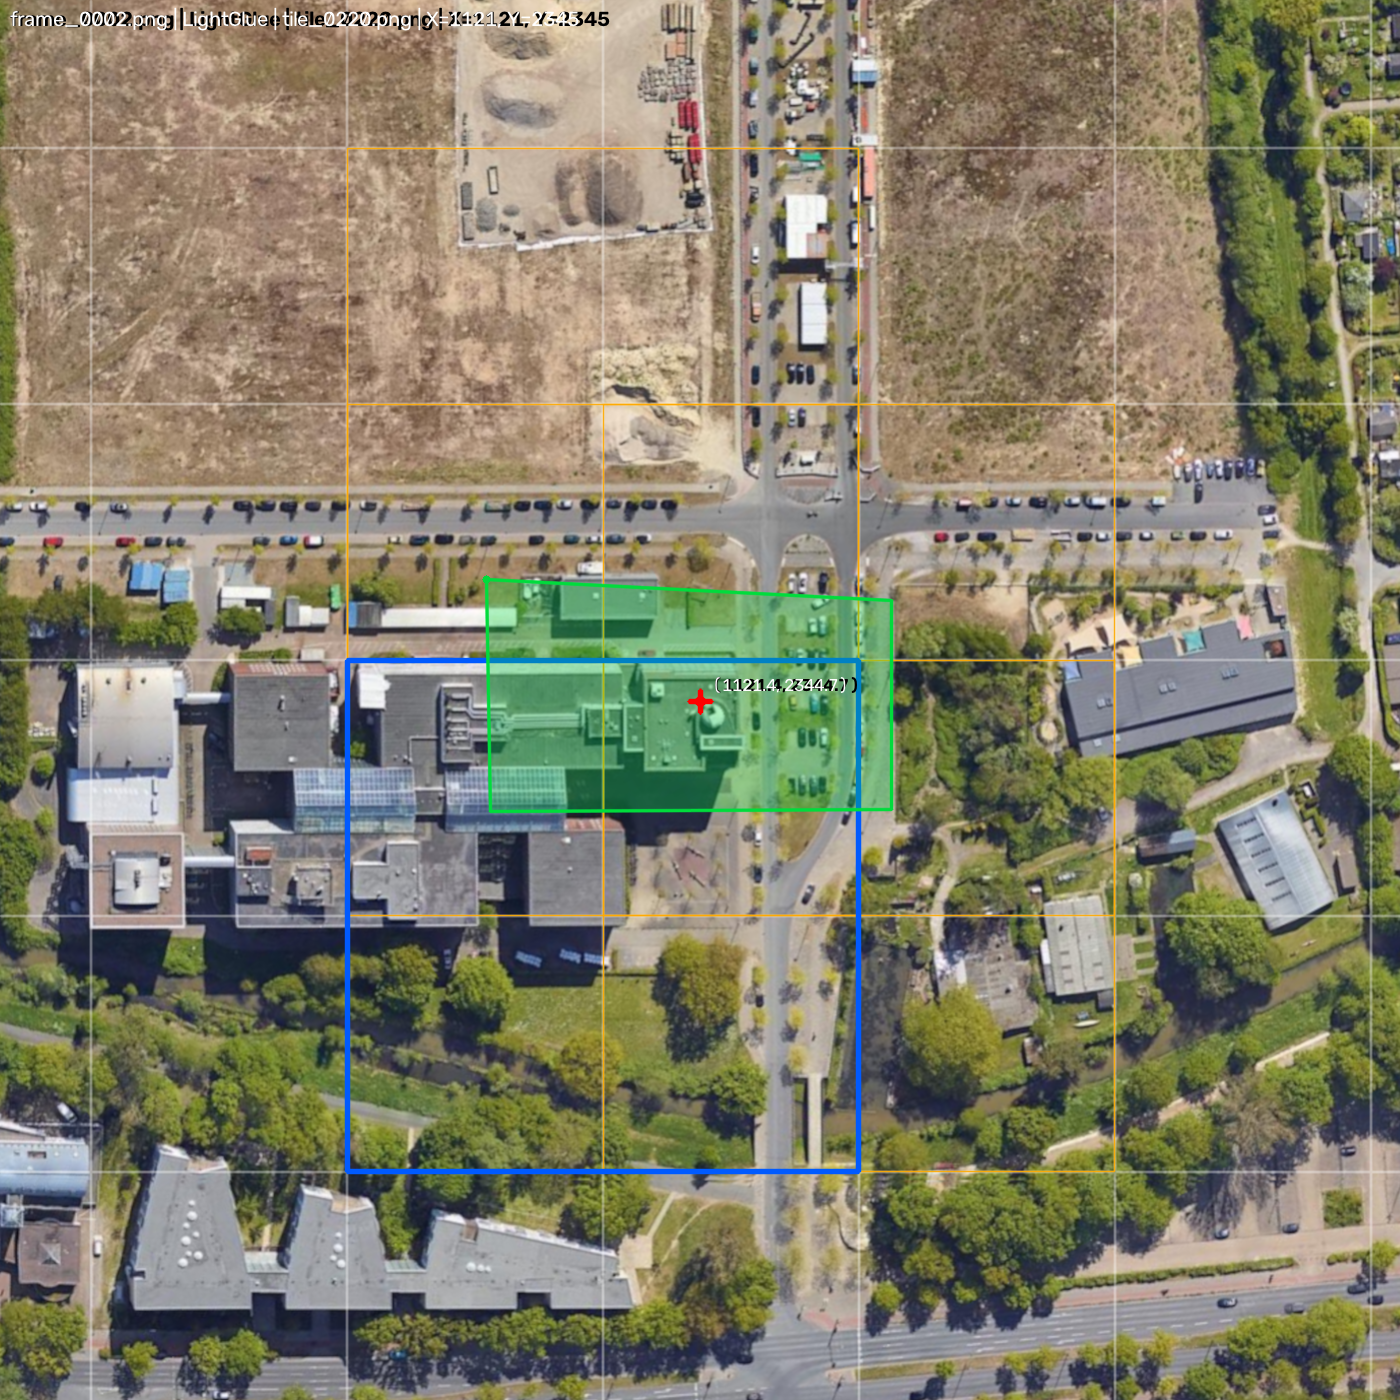
\includegraphics[width=0.75\linewidth]{images/master/global_loc_zoom.png}
    \caption{Результат автоматичного пошуку для кадру 2: сітка перевірених фрагментів, фрагменти, що пройшли фільтр (помаранчеві), фрагмент-переможець (синій), контур огляду камери (зелений) і центр кадру (червоний)}
    \label{fig:global-loc}
\end{figure}

В обох випадках переможцем став фрагмент, суміжний з еталонним фрагментом 196, який також містить центр кадру. Оцінка LoFTR відрізняється від калібрувальної оцінки $\approx(1110;\ 2330)$ на $\approx 3$~\px{}, оцінка LightGlue --- на $\approx 19$~\px{}. Усі фрагменти, що пройшли фільтр, перетинаються з місцем зйомки; жоден віддалений фрагмент фільтр не пройшов. Перегляд усієї карти з кешем ознак займає 33~с (85~мс на фрагмент), що прийнятно для початкової ініціалізації, але не для обробки кожного кадру. Це обґрунтовує використання трекера.

\subsection{Локалізація послідовності кадрів і вплив компенсації курсу}
\label{sec:exp-yaw}

Траєкторія польоту являє собою облітання кварталу: на північ, схід, південь і захід. Під час польоту курс змінюється приблизно так: $0^\circ \to 90^\circ \to 175^\circ \to -90^\circ \to -40^\circ$. Щоб оцінити внесок компенсації курсу, трекер (LightGlue + RANSAC) запущено на всіх 95 кадрах з компенсацією та без неї (табл.~\ref{tab:yaw}, рис.~\ref{fig:yaw}).

\begin{table}[H]
\centering
\caption{Вплив компенсації курсу на трекінг послідовності (LightGlue + RANSAC, 95 кадрів)}
\label{tab:yaw}
\begin{tabular}{lcc}
\toprule
& \textbf{Без компенсації} & \textbf{З компенсацією} \\
\midrule
\textsc{initialized} / \textsc{tracking} / \textsc{interpolated} / \textsc{lost} & 1 / 17 / 3 / 74 & 1 / 94 / 0 / 0 \\
Супровід утрачено & на кадрі 19, не відновлено & ні \\
Загальний час обробки & $\approx 41$~хв & 133~с \\
\bottomrule
\end{tabular}
\end{table}

\begin{figure}[H]
    \centering
    \begin{subfigure}{0.49\linewidth}
        \centering
        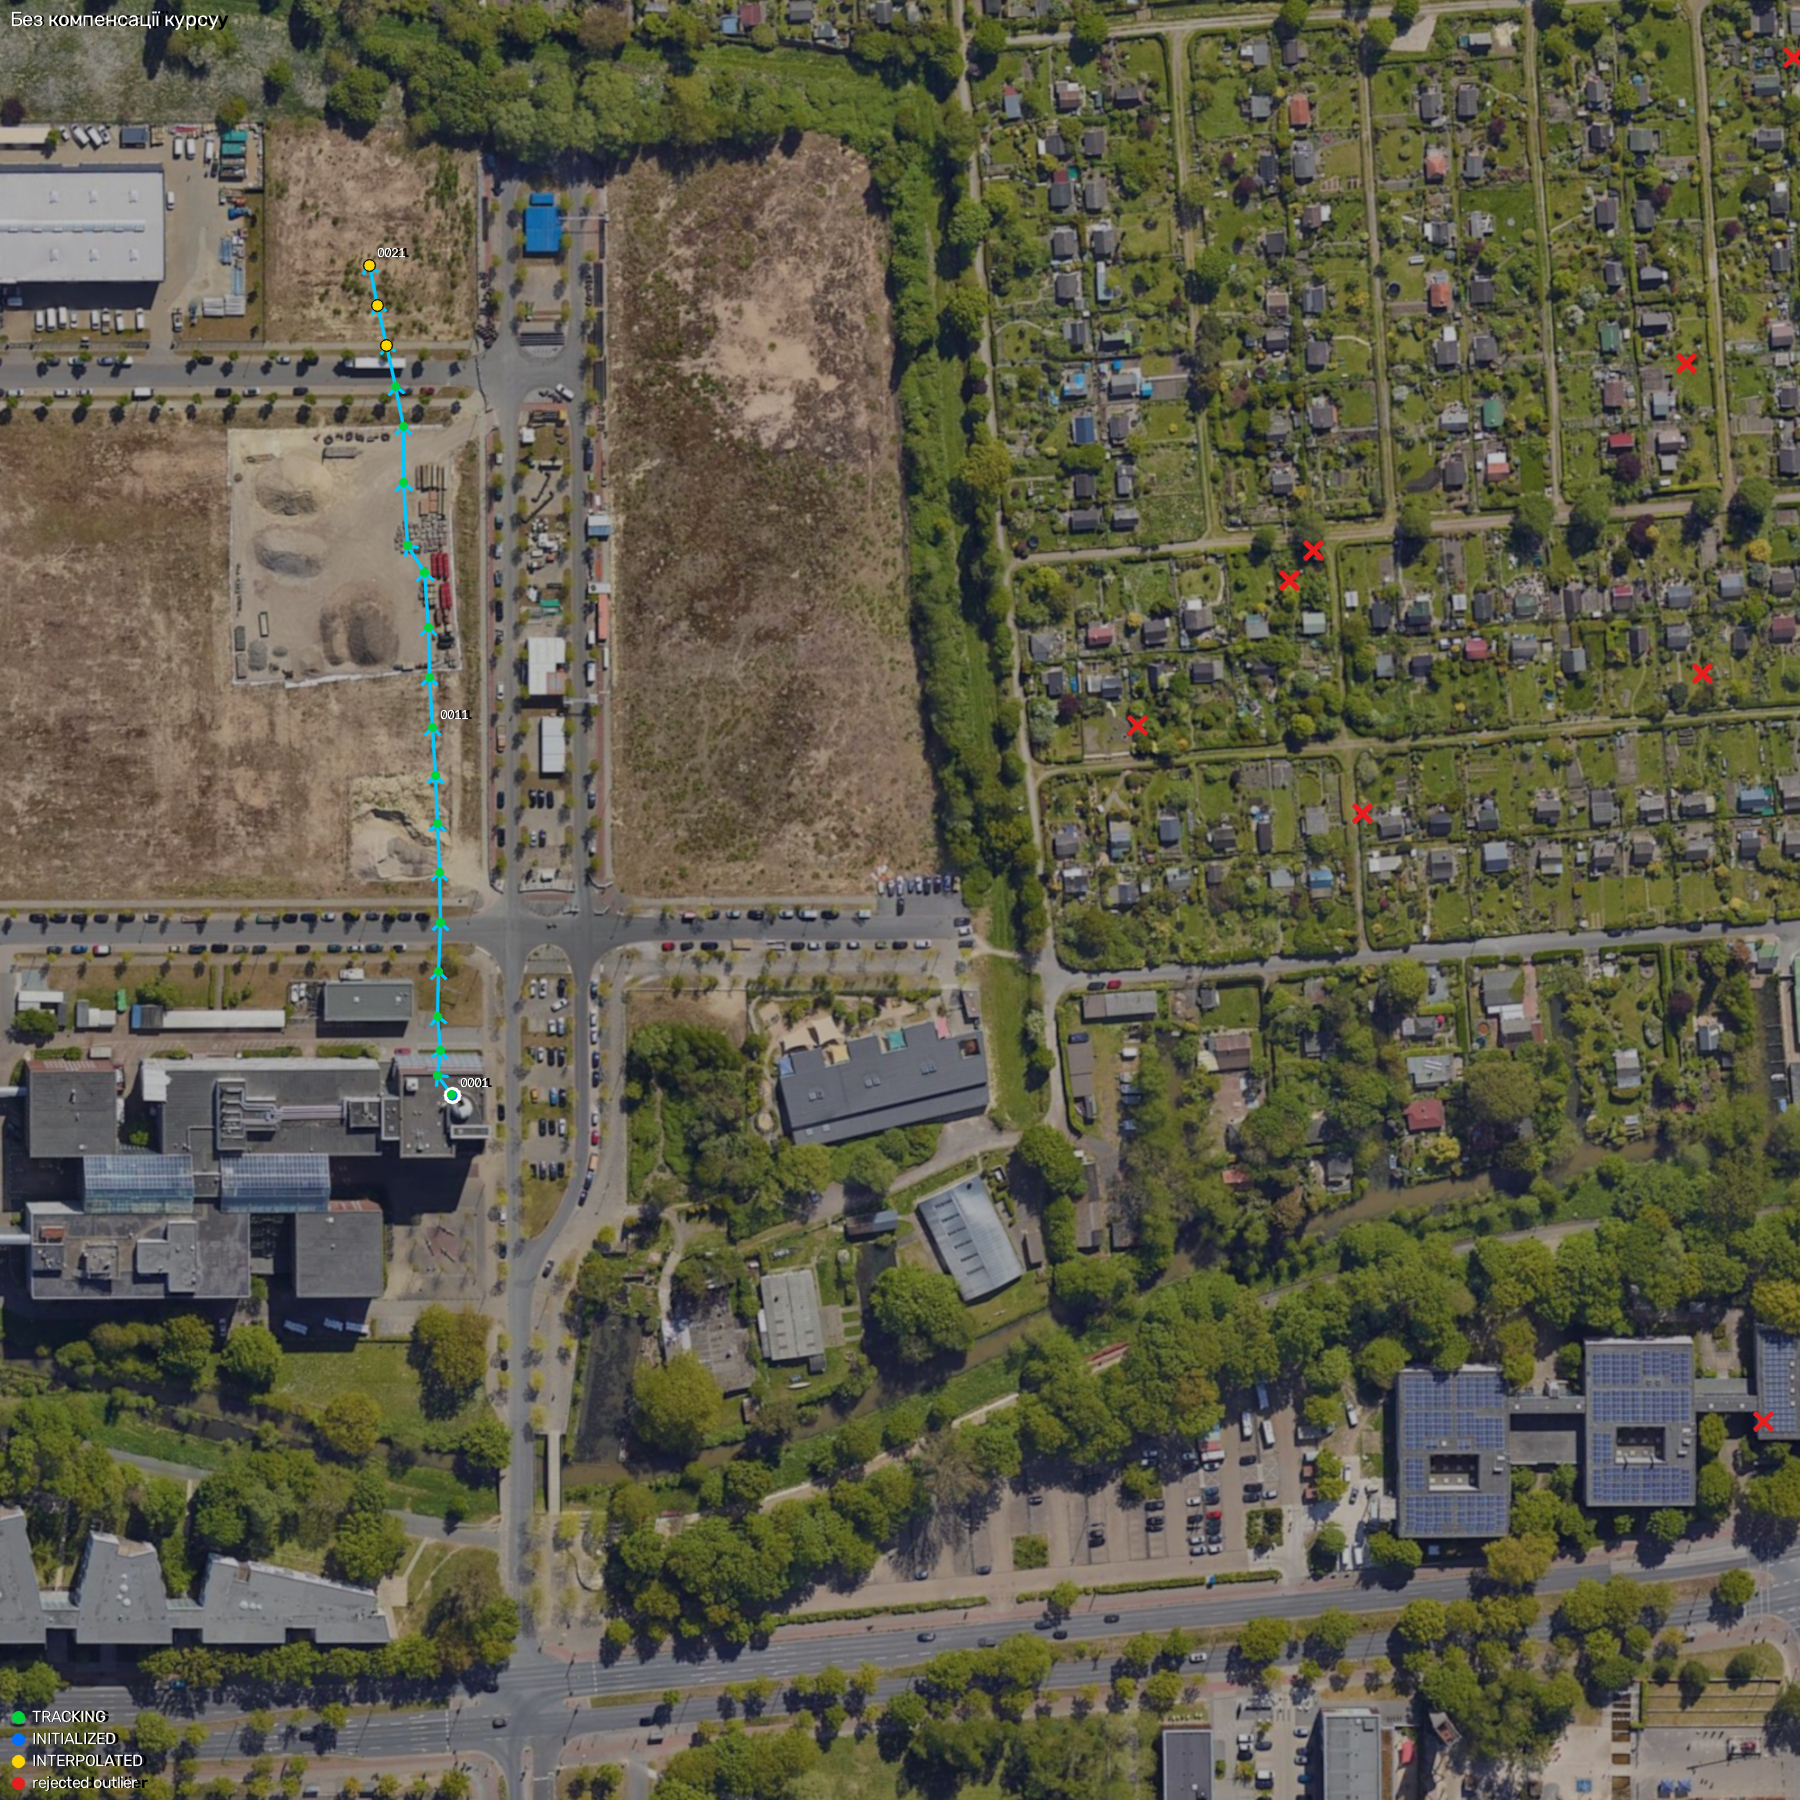
\includegraphics[width=\linewidth]{images/master/trajectory_no_yaw.png}
        \caption{без компенсації курсу}
    \end{subfigure}
    \hfill
    \begin{subfigure}{0.49\linewidth}
        \centering
        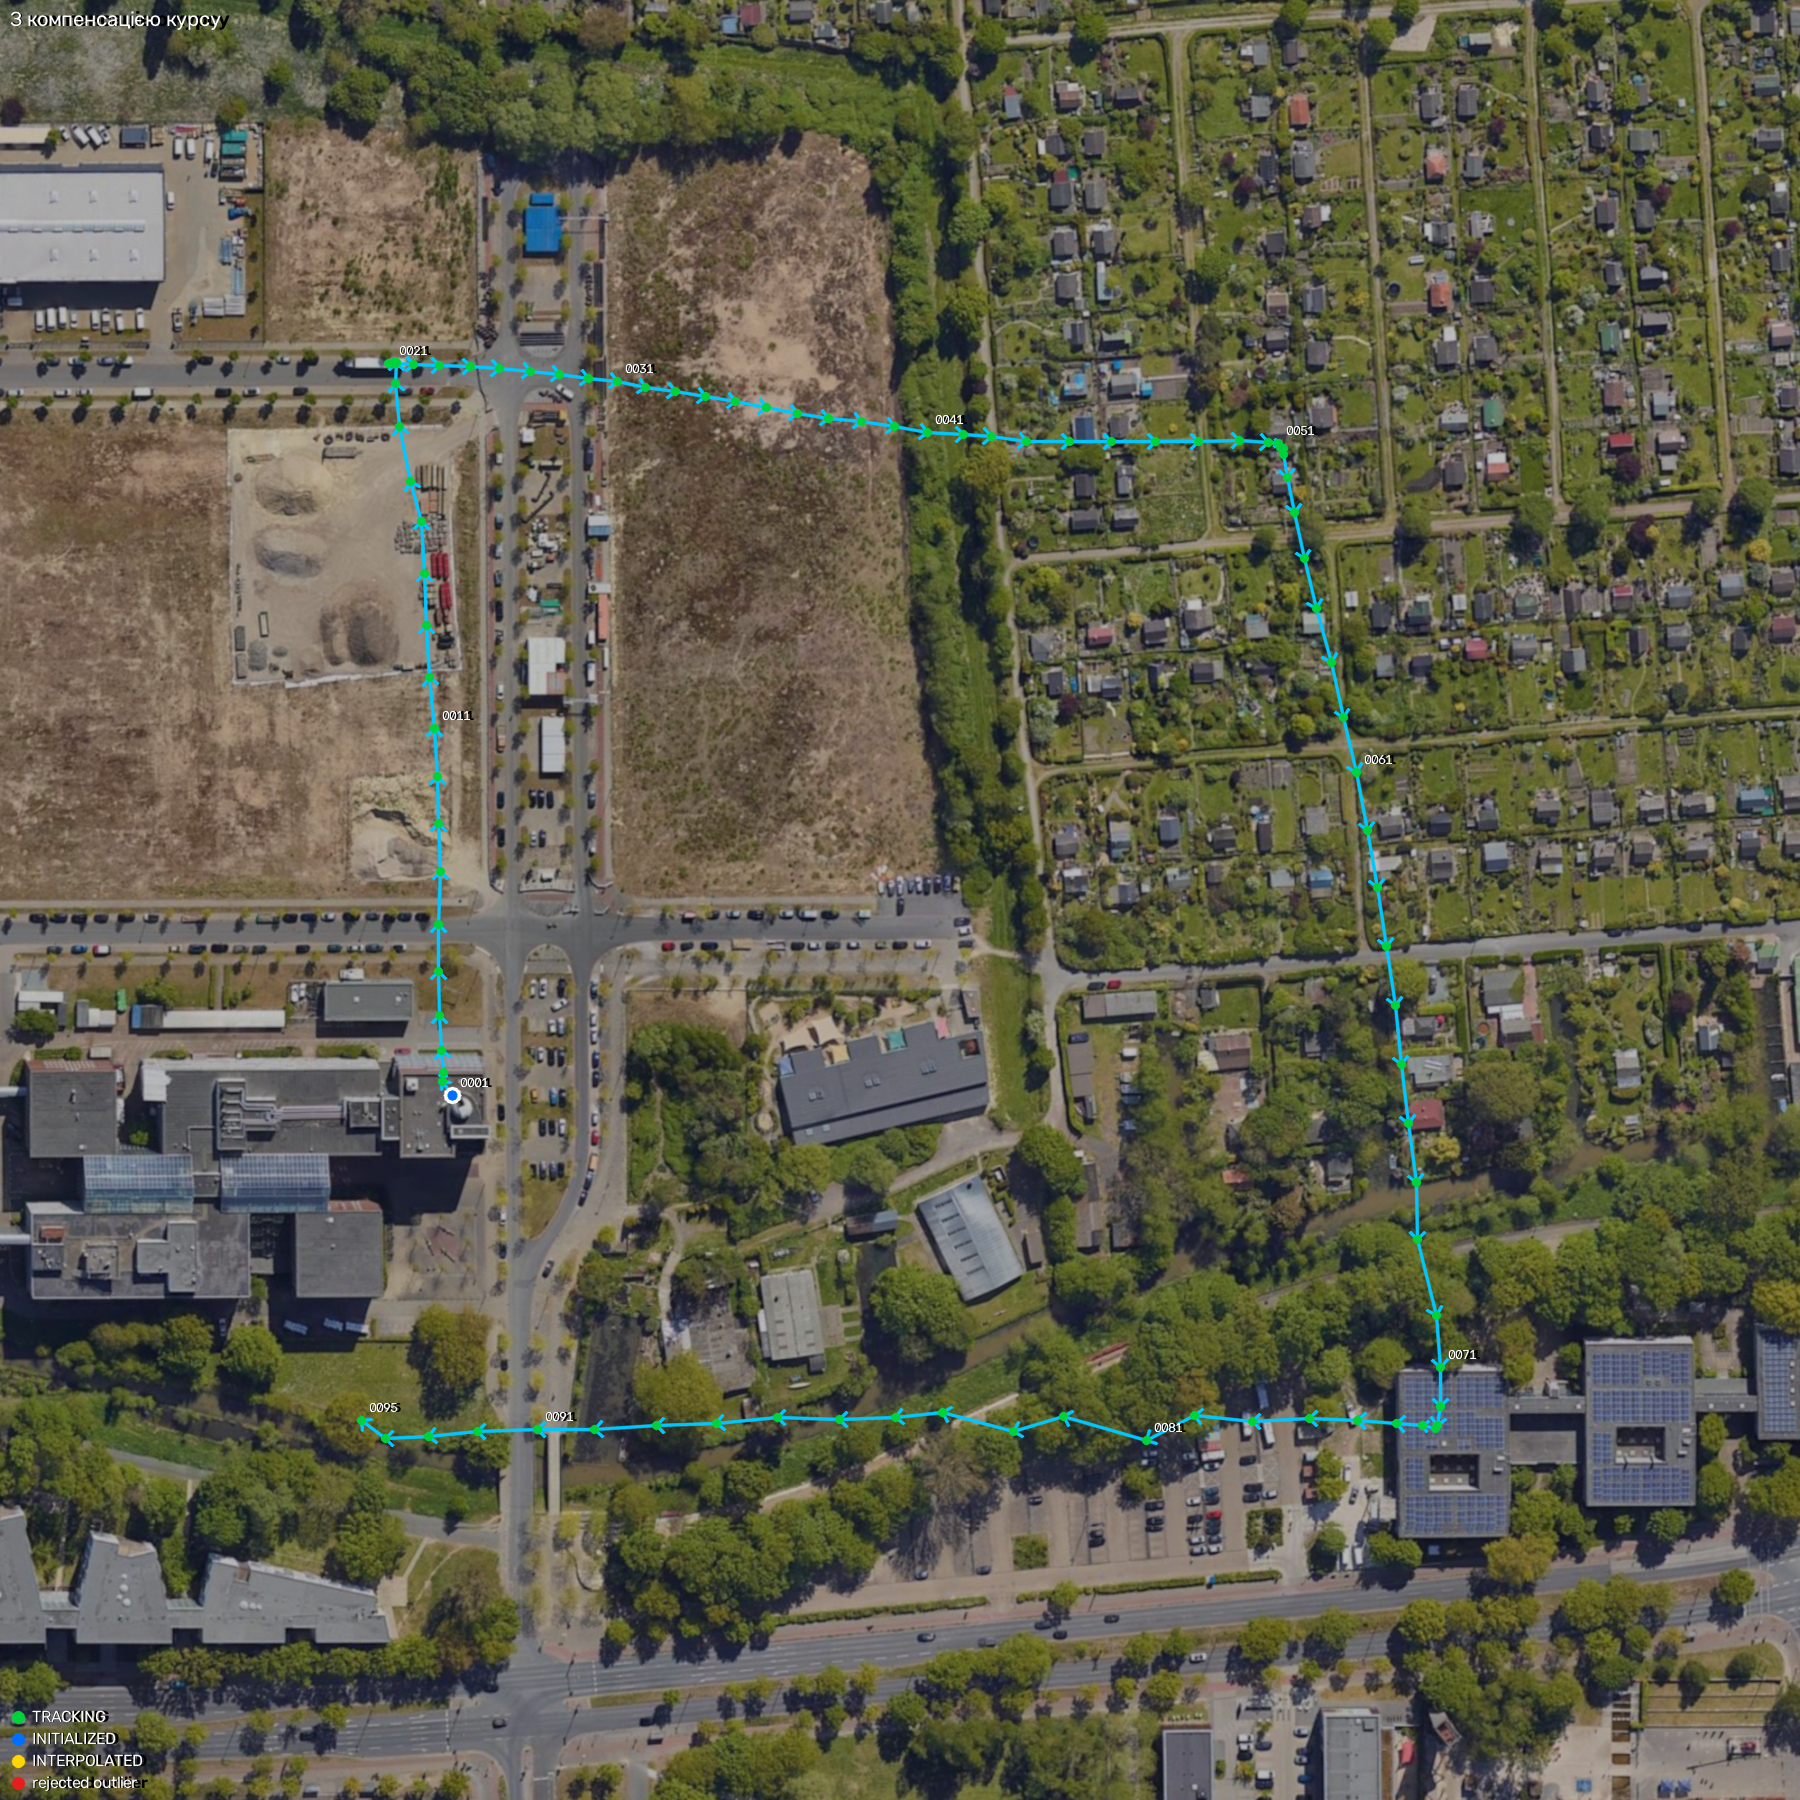
\includegraphics[width=\linewidth]{images/master/trajectory_with_yaw.png}
        \caption{з компенсацією курсу}
    \end{subfigure}
    \caption{Траєкторія, відновлена трекером: зелені точки --- \textsc{tracking}, жовті --- \textsc{interpolated}, червоні хрестики --- кандидати, відкинуті через низький бал або кінематичну перевірку}
    \label{fig:yaw}
\end{figure}

Без компенсації трекер утрачає супровід на першому розвороті (кадр 19, поворот кадру $\approx 50^\circ$). Глобальний пошук із курсом $0^\circ$ після цього вже не знаходить відповідного фрагмента. Кожен кадр у стані \textsc{lost} займає $\approx 32$~с, тому загальний час обробки зростає до 41~хв. З компенсацією всі чотири розвороти відстежено лише за прогнозом курсу; перебір додаткових гіпотез курсу знадобився для одного кадру. Компенсація курсу виявилася необхідною умовою роботи системи на реальному польоті.

\subsection{Порівняння методів LightGlue і LoFTR}
\label{sec:exp-methods}

Усі чотири конфігурації відстежили всю послідовність: 94 кадри зі статусом \textsc{tracking} і один \textsc{initialized}, лише для LightGlue + MAGSAC++ один кадр екстрапольовано. Кінематична перевірка жодного разу не відкинула оцінку, а повторна глобальна ініціалізація не знадобилася. Показники трекінгу та точності наведено в табл.~\ref{tab:tracking} і \ref{tab:accuracy}; відновлені траєкторії разом з еталоном --- на рис.~\ref{fig:traj-gt}, похибки на опорних кадрах --- на рис.~\ref{fig:error}.

\begin{table}[H]
\centering
\caption{Показники трекінгу послідовності з 95 кадрів}
\label{tab:tracking}
\small
\begin{tabular}{lcccccc}
\toprule
\multirow{2}{*}{\textbf{Конфігурація}} & \multicolumn{2}{c}{\textbf{Час кадру, с}} & \textbf{Глобальний} & \multirow{2}{*}{\textbf{Медіана} $N_{\text{in}}$} & \multirow{2}{*}{$\bar{r}$} & \multirow{2}{*}{$\bar{e}$, \px{}} \\
& середній & $P_{90}$ & \textbf{пошук, с} & & & \\
\midrule
LightGlue + RANSAC & 1,08 & 1,40 & 38,3 & 81 & 0,48 & 1,65 \\
LightGlue + MAGSAC++ & 0,78 & 1,02 & 20,1 & 87 & 0,50 & 1,73 \\
LoFTR + RANSAC & 2,72 & 2,93 & 127,9 & 316 & 0,59 & 1,27 \\
LoFTR + MAGSAC++ & 2,27 & 2,49 & 87,5 & 353 & 0,61 & 1,33 \\
\bottomrule
\end{tabular}
\end{table}

\begin{table}[H]
\centering
\caption{Похибка локалізації на 18 надійних опорних кадрах, \px{}}
\label{tab:accuracy}
\small
\begin{tabular}{lccccccc}
\toprule
\textbf{Конфігурація} & \textbf{Середня} & \textbf{Медіана} & \textbf{RMSE} & $P_{90}$ & \textbf{Макс.} & \textbf{S@10} & \textbf{S@25} \\
\midrule
LightGlue + RANSAC & 7,2 & 6,0 & 9,5 & 16,8 & 22,9 & 83\,\% & 100\,\% \\
LightGlue + MAGSAC++ & 7,5 & 5,7 & 10,2 & 16,5 & 27,5 & 78\,\% & 94\,\% \\
LoFTR + RANSAC & 4,9 & 3,1 & 7,3 & 9,0 & 24,2 & 94\,\% & 100\,\% \\
LoFTR + MAGSAC++ & 5,2 & 2,9 & 8,9 & 8,2 & 33,2 & 94\,\% & 94\,\% \\
\bottomrule
\end{tabular}
\end{table}

\begin{figure}[H]
    \centering
    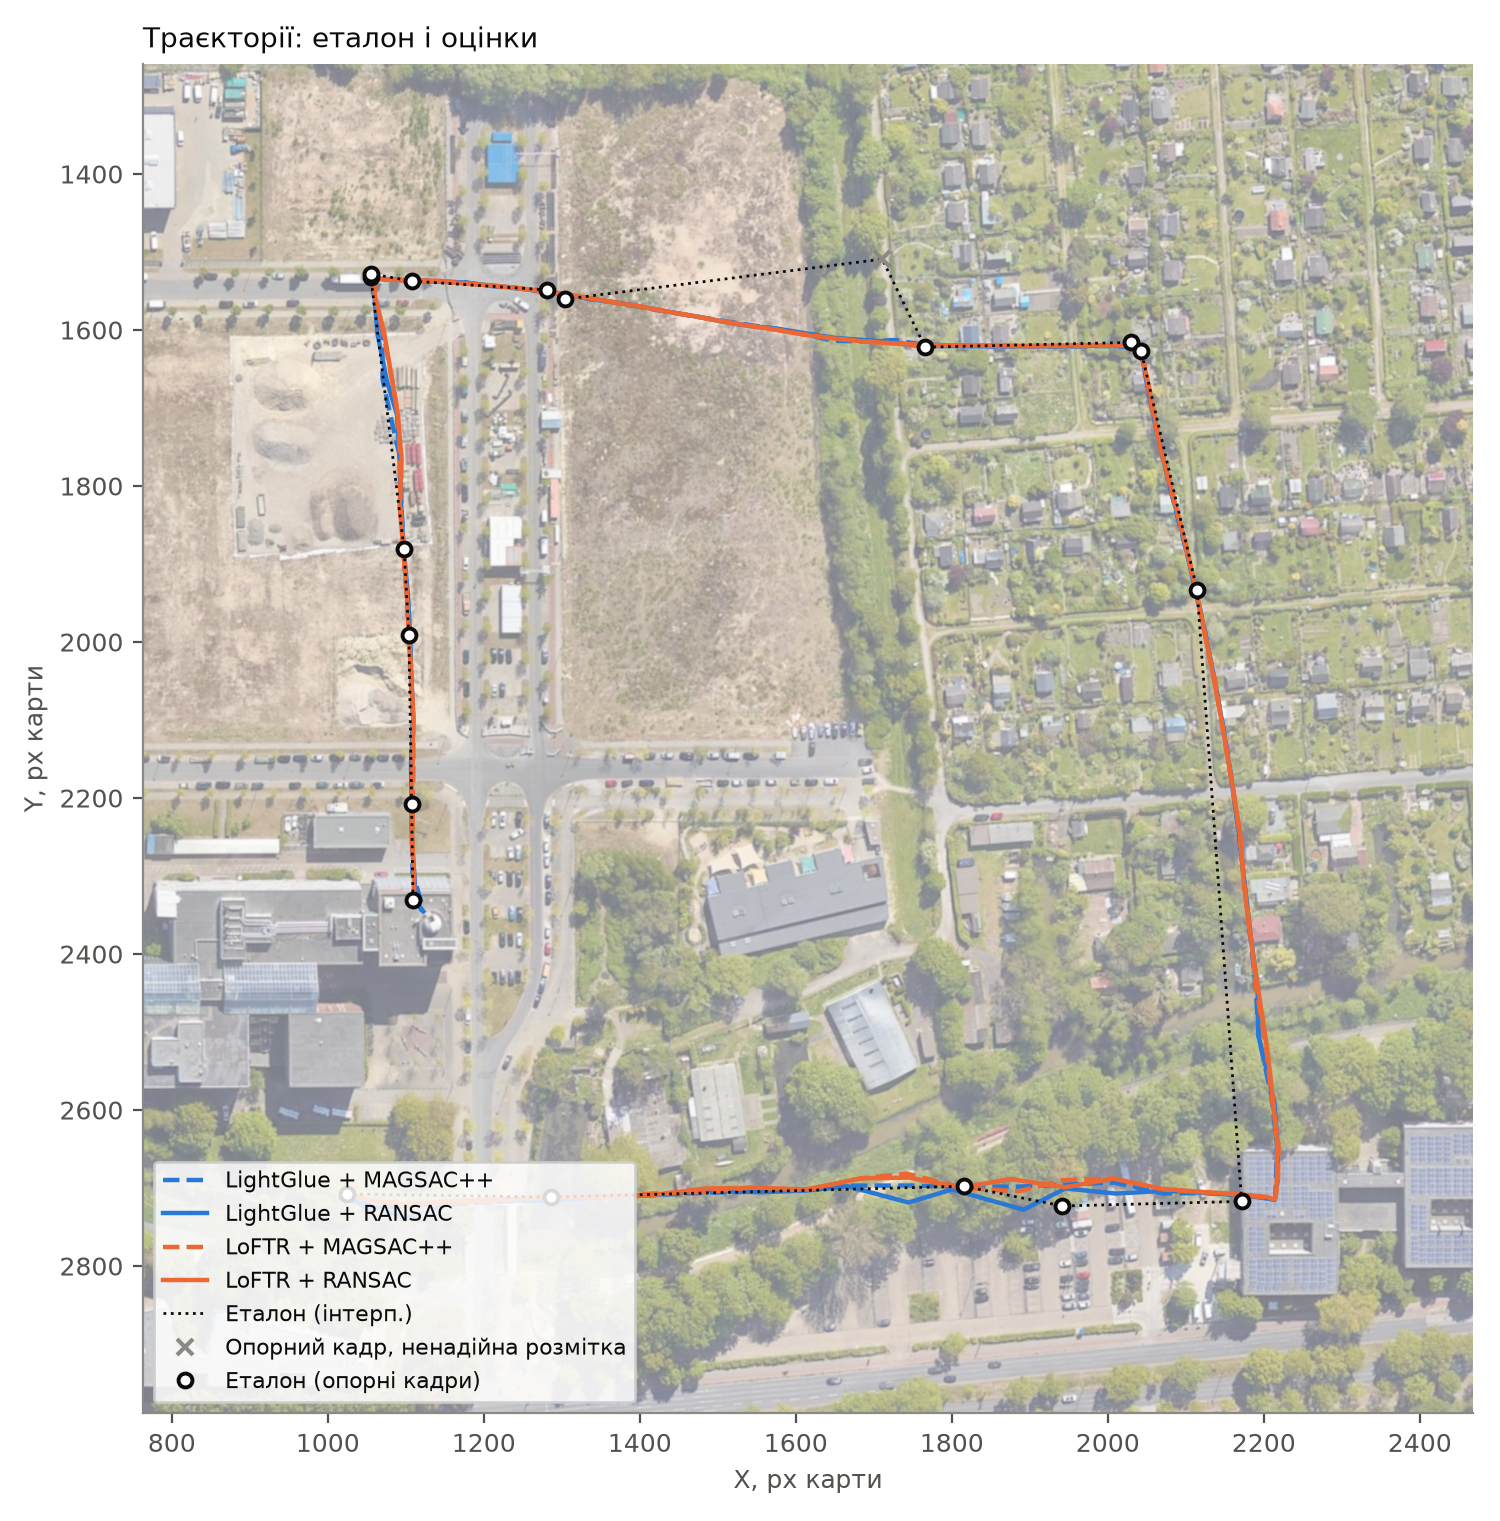
\includegraphics[width=0.8\linewidth]{images/master/trajectories_vs_gt.png}
    \caption{Траєкторії, відновлені чотирма конфігураціями, та еталонні положення опорних кадрів}
    \label{fig:traj-gt}
\end{figure}

\begin{figure}[H]
    \centering
    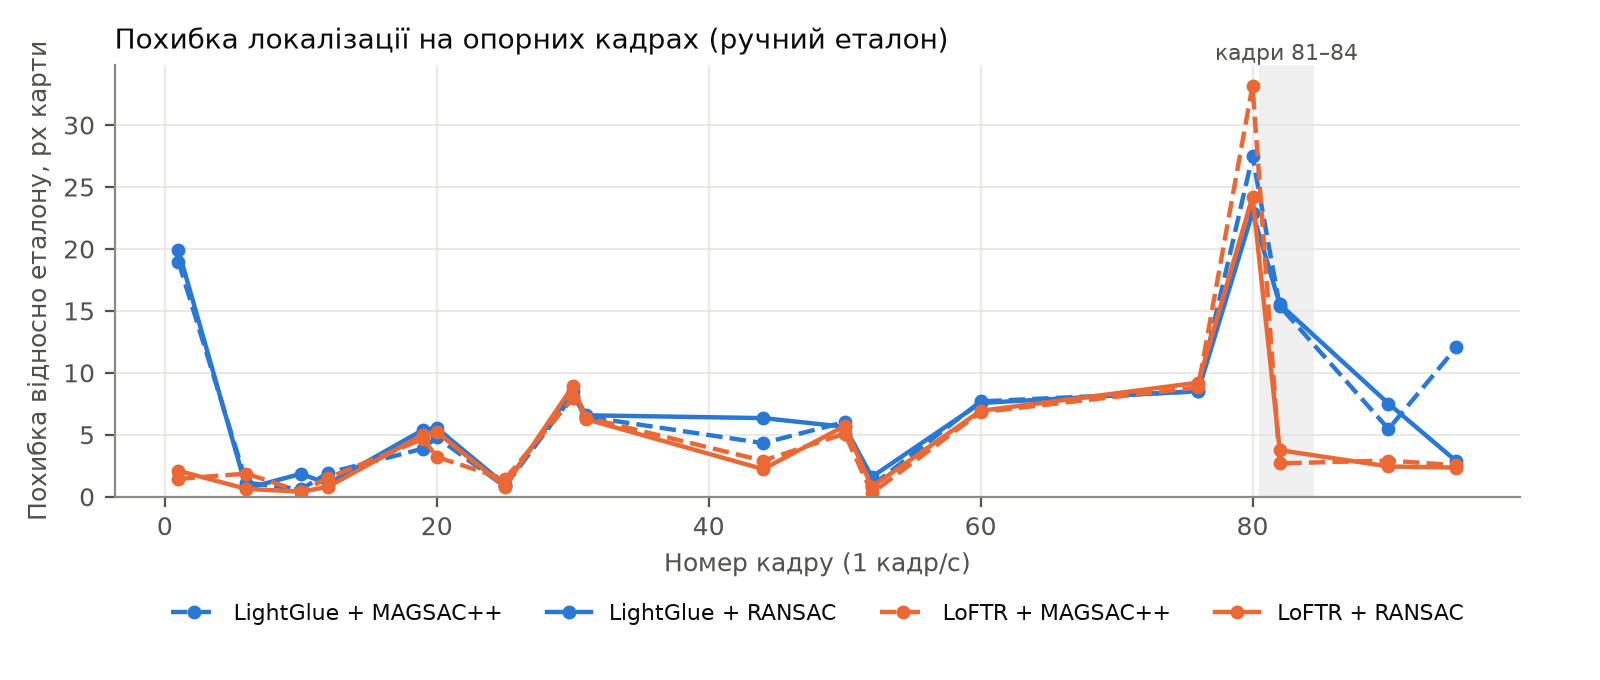
\includegraphics[width=\linewidth]{images/master/error_over_time.png}
    \caption{Похибка локалізації на опорних кадрах уздовж польоту}
    \label{fig:error}
\end{figure}

\textbf{Точність.}\\
LoFTR забезпечує меншу медіанну похибку, ніж LightGlue: $\approx 3$~\px{} проти $\approx 6$~\px{}. Частка кадрів із похибкою не більше 10~\px{} становить 94\,\% проти 78--83\,\%. У парному порівнянні з однаковим оцінювачем RANSAC LoFTR точніший на 14 з 18 опорних кадрів (знаковий тест, $p = 0{,}031$), з MAGSAC++ --- на 13 з 18 ($p = 0{,}096$). На більшості кадрів різниця між методами не перевищує 1--2~\px{}, тобто є порівнянною з невизначеністю еталона. Перевагу LoFTR формують насамперед кілька складних кадрів:
\begin{itemize}
    \item кадр 1: 19,9~\px{} у LightGlue проти 2,1~\px{} у LoFTR --- LightGlue під час ініціалізації оцінює гомографію площини даху високої будівлі (див. п.~\ref{sec:exp-pair});
    \item кадр 82 поблизу масиву дерев: 15,5~\px{} проти 3,8~\px{};
    \item кадр 90: 7,5~\px{} проти 2,4~\px{}.
\end{itemize}

На кадрі 80 усі чотири конфігурації мають близьку похибку 23--33~\px{}. Збіг похибки незалежних методів вказує на систематичну причину, спільну для всіх. Найімовірніше, це неточність еталона: усі точки розмітки цього кадру розташовані в його лівій третині (дорога й паркінг), права частина кадру зайнята деревами, а центр кадру екстрапольовано. Без кадру 80 середня похибка становить 6,2--6,3~\px{} для LightGlue і 3,6--3,7~\px{} для LoFTR; максимальна похибка LoFTR зменшується до 9,2~\px{}.

\textbf{Кількість відповідностей і швидкодія.}\\
LoFTR знаходить у 3,6--4 рази більше геометрично узгоджених відповідностей (медіана 316--353 проти 81--87) з більшою їх часткою та меншою похибкою репроєкції. Водночас LoFTR у 2,5--2,9 раза повільніший у режимі трекінгу (2,3--2,7~с проти 0,8--1,1~с на кадр) і в 3,3 (RANSAC) та 4,4 (MAGSAC++) раза повільніший під час глобального пошуку, оскільки для нього неможливе кешування ознак фрагментів. Між собою траєкторії конфігурацій відрізняються з медіаною 0,8--1,7~\px{}; найбільші розбіжності (19--43~\px{}) припадають на кадри 79--83 над деревами.

\subsection{Порівняння оцінювачів RANSAC і MAGSAC++}

Розподіл часу обробки кадру в режимі трекінгу наведено на рисунку~\ref{fig:timing}.

\begin{figure}[H]
    \centering
    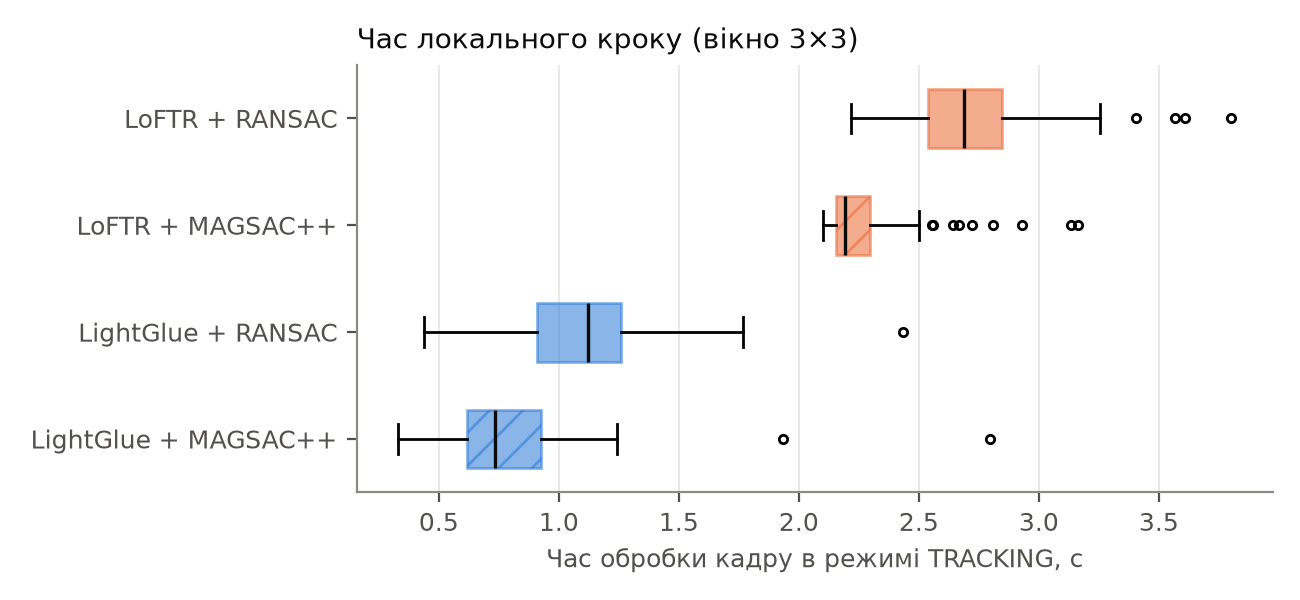
\includegraphics[width=0.75\linewidth]{images/master/timing_local.png}
    \caption{Час обробки кадру в режимі \textsc{tracking} для чотирьох конфігурацій}
    \label{fig:timing}
\end{figure}

Заміна RANSAC на MAGSAC++ скорочує час кадру на 28\,\% для LightGlue (1,08 $\to$ 0,78~с) і на 17\,\% для LoFTR (2,72 $\to$ 2,27~с), а час глобального пошуку --- у 1,9 і 1,5 раза відповідно. Виграш отримано насамперед на фрагментах, які не містять місця зйомки: на таких фрагментах реалізація RANSAC в OpenCV не може достроково зупинитися і виконує всі 5000 ітерацій, тоді як MAGSAC++ завершується за кілька мілісекунд.

Статистично значущої різниці в точності не виявлено. У парному порівнянні MAGSAC++ точніший за RANSAC на 12 з 18 кадрів для LightGlue ($p = 0{,}24$) і на 9 з 18 для LoFTR ($p = 1{,}0$), медіанна різниця не перевищує 0,2~\px{}. Траєкторії, отримані з різними оцінювачами, відрізняються з медіаною 1,2~\px{} (LightGlue) і 0,8~\px{} (LoFTR). Таким чином, MAGSAC++ дає змогу пришвидшити систему без втрати точності. Конфігурація LightGlue + MAGSAC++ --- єдина, що забезпечує обробку кадру не довше 1~с (середнє 0,78~с, $P_{90}$ 1,02~с).

\subsection{Стійкість до спотворень зображення}
\label{sec:exp-robust}

Для 19 кадрів (кожен п'ятий кадр послідовності) штучно застосовано спотворення до оригінального кадру $1920 \times 1080$:
\begin{itemize}
    \item зниження яскравості $I' = \alpha I$;
    \item зниження контрасту $I' = \alpha (I - \mu) + \mu$, де $\mu$ --- середнє значення каналу;
    \item адитивний гауссів шум;
    \item лінійне розмиття руху;
    \item поворот кадру без компенсації;
    \item помилка у заданому масштабі $s_f$.
\end{itemize}
Пул фрагментів і компенсація курсу були такими самими, як у трекері на відповідному кадрі. Для кожного кадру обчислено відношення $N_{\text{in}}$ до значення для неспотвореного кадру та зміщення знайденого центру. Результати наведено в табл.~\ref{tab:robust} і на рис.~\ref{fig:robust}.

\begin{table}[H]
\centering
\caption{Стійкість до спотворень (19 кадрів): частка локалізованих кадрів і медіанне відношення $N_{\text{in}} / N_{\text{in}}^{\text{без спотв.}}$}
\label{tab:robust}
\small
\begin{tabular}{lcccc}
\toprule
\multirow{2}{*}{\textbf{Спотворення}} & \multicolumn{2}{c}{\textbf{LightGlue}} & \multicolumn{2}{c}{\textbf{LoFTR}} \\
\cmidrule(lr){2-3}\cmidrule(lr){4-5}
& локалізовано & відношення & локалізовано & відношення \\
\midrule
яскравість $\alpha = 0{,}7$ / $0{,}5$ & 100 / 100\,\% & 1,00 / 1,01 & 100 / 100\,\% & 0,97 / 0,97 \\
контраст $\alpha = 0{,}7$ / $0{,}5$ & 100 / 100\,\% & 1,02 / 0,99 & 100 / 100\,\% & 1,00 / 0,97 \\
шум $\sigma = 10$ / $25$ & 95 / 95\,\% & 0,99 / 0,92 & 100 / 95\,\% & 1,02 / 0,95 \\
розмиття 5 / 9 пікселів & 100 / 100\,\% & 1,02 / 1,02 & 100 / 100\,\% & 1,02 / 1,04 \\
поворот $15^\circ$ / $30^\circ$ & 95 / 95\,\% & 1,03 / 0,99 & 95 / 95\,\% & 0,82 / 0,52 \\
поворот $45^\circ$ & 53\,\% & 0,35 & 11\,\% & 0 \\
поворот $90^\circ$ & 0\,\% & 0 & 0\,\% & 0 \\
масштаб $\times 0{,}8$ / $\times 1{,}25$ & 100 / 95\,\% & 0,68 / 1,29 & 100 / 100\,\% & 0,71 / 1,05 \\
\bottomrule
\end{tabular}
\end{table}

\begin{figure}[H]
    \centering
    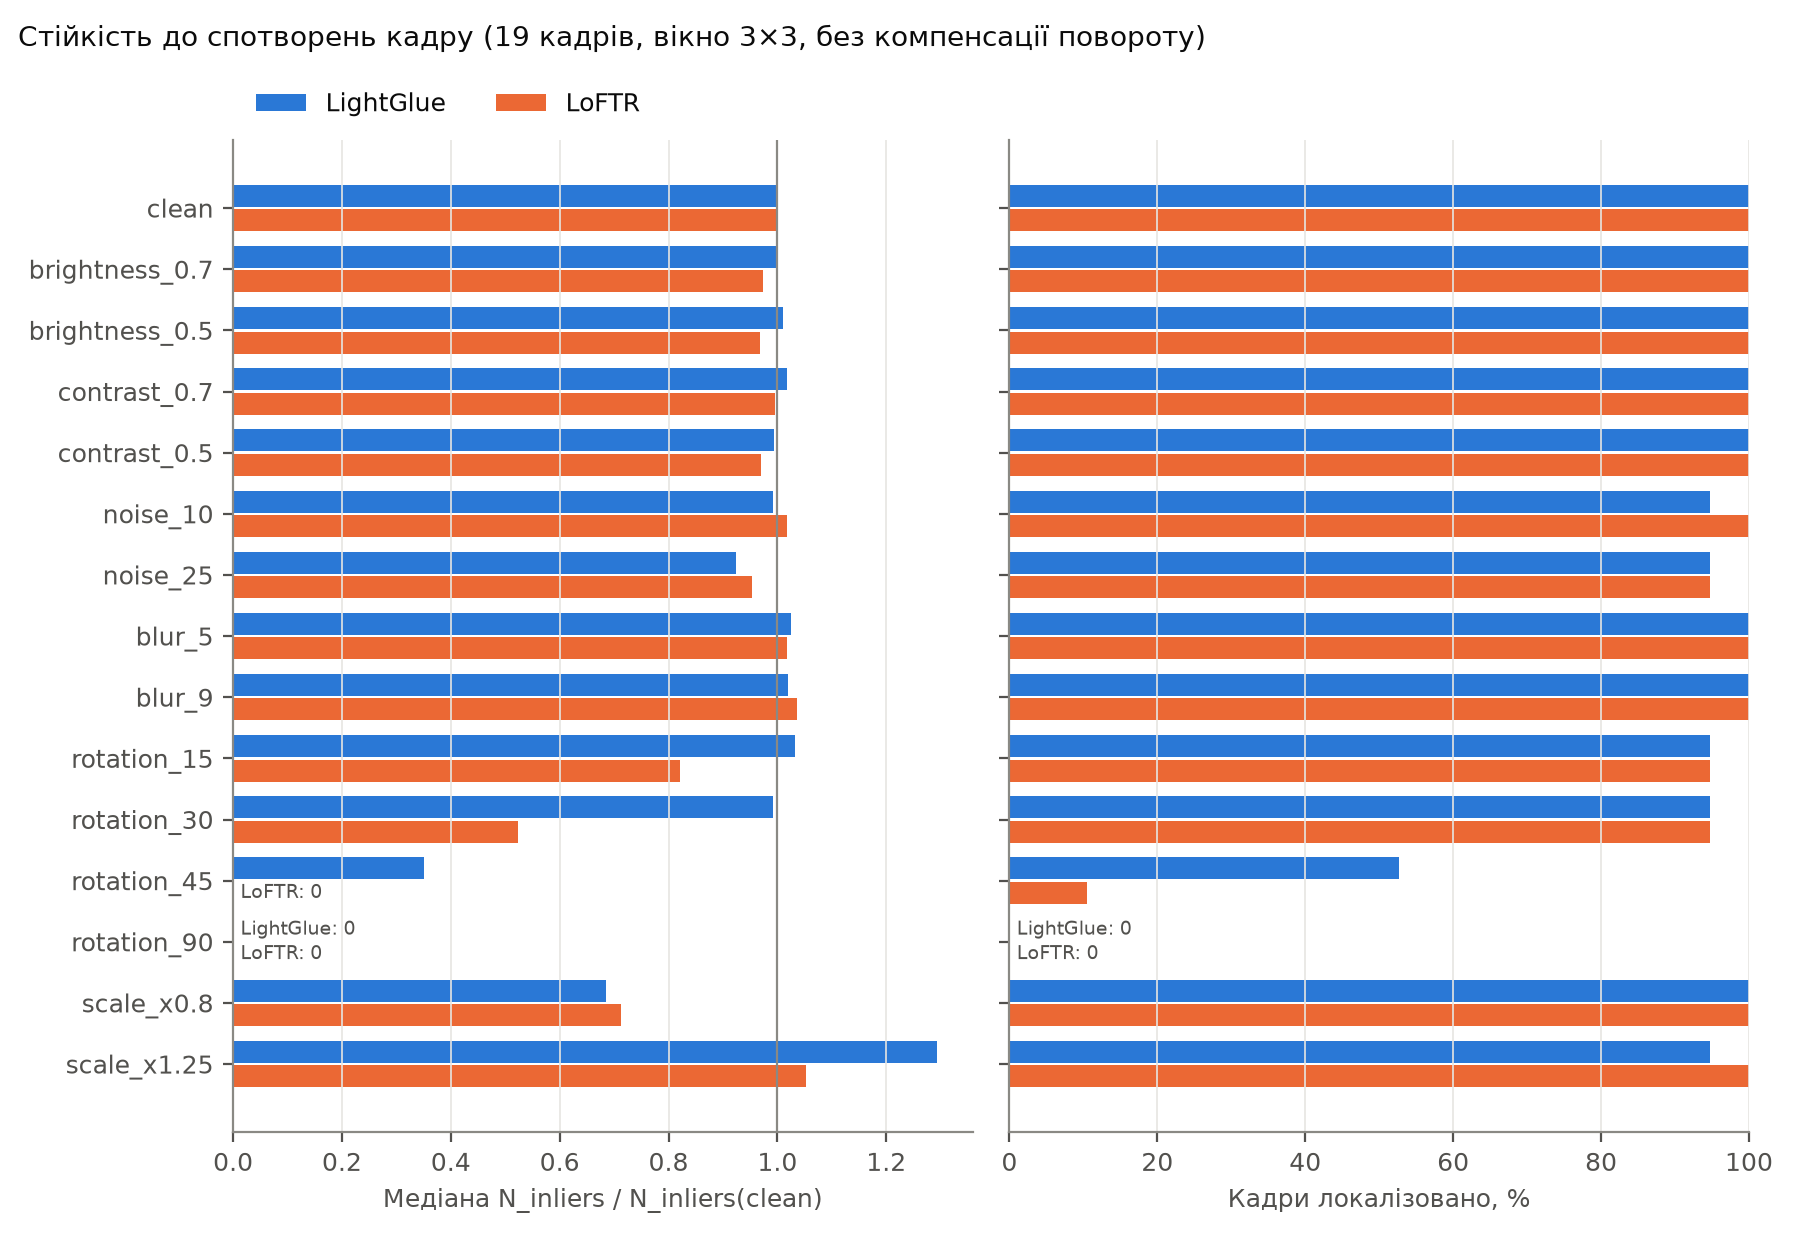
\includegraphics[width=\linewidth]{images/master/robustness.png}
    \caption{Стійкість методів до спотворень кадру}
    \label{fig:robust}
\end{figure}

Зміни яскравості й контрасту, гауссів шум і розмиття в досліджених межах практично не впливають на результат: кількість геометрично узгоджених відповідностей зберігається, а медіанне зміщення центру не перевищує 1,5~\px{}. Слабкий вплив розмиття частково пояснюється тим, що після масштабування кадру з коефіцієнтом 0,27 ядро 9 пікселів зменшується до $\approx 2{,}4$ пікселя.

Визначальним чинником виявився поворот кадру. LightGlue зберігає працездатність до $30^\circ$, а LoFTR втрачає половину відповідностей уже при $30^\circ$. При $45^\circ$ локалізовано лише 53\,\% (LightGlue) і 11\,\% (LoFTR) кадрів, при $90^\circ$ --- жодного. Ці результати кількісно обґрунтовують компенсацію курсу, описану в п.~\ref{sec:tracking}. Похибка масштабу на 20--25\,\% не призводить до втрати локалізації, але зменшення заданого масштабу на 20\,\% скорочує кількість відповідностей приблизно на 30\,\%.

\subsection{Аналіз проблемних ділянок місцевості}

Для кожного кадру за контуром огляду обчислено дві ознаки ділянки ортофотоплану:
\begin{itemize}
    \item частку рослинності за індексом Excess Green $\text{ExG} = 2g - r - b$ у хроматичних координатах \cite{exg} (піксель вважається рослинністю, якщо $\text{ExG} > 0{,}05$);
    \item текстурованість --- середній модуль градієнта Собеля яскравості.
\end{itemize}
Залежність кількості геометрично узгоджених відповідностей від номера кадру та частки рослинності наведено на рисунку~\ref{fig:terrain}, кореляції --- у табл.~\ref{tab:terrain}.

\begin{figure}[H]
    \centering
    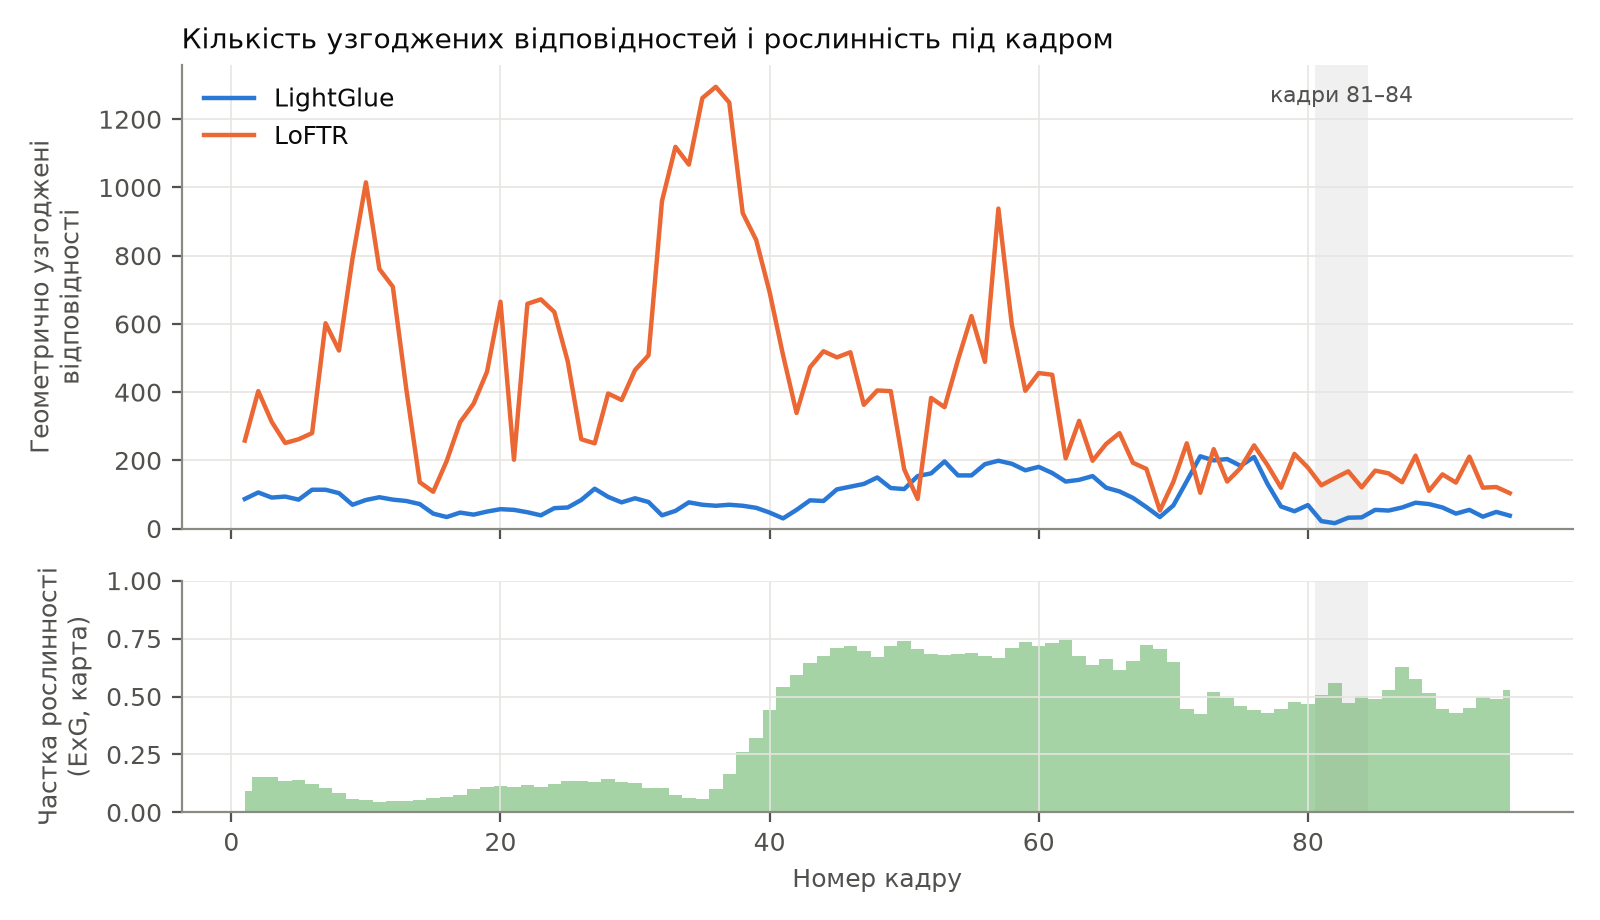
\includegraphics[width=\linewidth]{images/master/inliers_vs_terrain.png}
    \caption{Кількість геометрично узгоджених відповідностей уздовж польоту (вгорі) і частка рослинності під кадром (внизу); сірим виділено кадри 81--84}
    \label{fig:terrain}
\end{figure}

\begin{table}[H]
\centering
\caption{Зв'язок кількості геометрично узгоджених відповідностей з ознаками місцевості (кореляція Спірмена $\rho$, RANSAC)}
\label{tab:terrain}
\begin{tabular}{lcccc}
\toprule
\textbf{Метод} & $\rho$ (рослинність) & $\rho$ (текстура) & \textbf{Медіана} $N_{\text{in}}$, кадри 81--84 & \textbf{Медіана} $N_{\text{in}}$, усі \\
\midrule
LightGlue & $+0{,}37$ & $+0{,}65$ & 27 & 81 \\
LoFTR & $-0{,}29$ & $+0{,}29$ & 138 & 316 \\
\bottomrule
\end{tabular}
\end{table}

На ділянці кадрів 81--84 (паркінг і канал, оточені деревами) кількість геометрично узгоджених відповідностей падає втричі для LightGlue і вдвічі для LoFTR. Саме тут методи найбільше розходяться між собою. Водночас частка рослинності під кадром сама по собі не пояснює це падіння: для LightGlue кореляція з нею навіть додатна, оскільки дачні ділянки з будівлями мають високу частку рослинності, але багаті на деталі. Кращим предиктором для LightGlue є текстурованість ($\rho = 0{,}65$); для LoFTR зв'язок з обома ознаками слабкий. Імовірною причиною падіння на кадрах 81--84 є сезонна різниця крон листяних дерев (на відео --- без листя, на карті --- з листям), однак підтвердження цієї гіпотези потребує окремого дослідження.

% TODO: експерименти з розміром фрагмента (256/512/768/1024) і часткою перекриття (25/50 %),
%       передбачені технічним завданням, ще не проведено. Після їх виконання додати
%       підрозділ з результатами (див. обмеження нижче щодо розміру фрагмента 512).

\subsection{Обмеження розробленої системи}

Під час експериментів виявлено такі обмеження:
\begin{itemize}
    \item \textbf{Плоска модель сцени.} Гомографія описує лише площину. Високі будівлі спричиняють паралакс, і RANSAC може оцінити площину даху замість площини землі (кадр 1 у LightGlue, кадр 2 у LoFTR).
    \item \textbf{Розмір фрагмента.} Контур огляду кадру ($\approx 518 \times 292$~\px{}) ширший за фрагмент 512~\px{}, тому жоден фрагмент не містить кадр повністю.
    \item \textbf{Фіксований масштаб.} Масштаб кадру $s_f$ відкалібровано на одному кадрі, і він вважається сталим. Під час польоту оцінений масштаб гомографії змінювався в межах 0,20--0,32 (медіана 0,269), проте в трекері він не уточнюється.
    \item \textbf{Чутливість до повороту.} Без компенсації курсу обидва методи непрацездатні при повороті кадру на $45^\circ$ і більше; перший глобальний пошук виконується з курсом $0^\circ$.
    \item \textbf{Швидкодія.} Повний перебір карти займає 20--128~с залежно від конфігурації. Обмеження 1~с на кадр у режимі трекінгу на використаному GPU виконує лише LightGlue + MAGSAC++.
    \item \textbf{Одиниці вимірювання.} Без просторової прив'язки ортофотоплану похибки визначено в пікселях карти; переведення в метри потребує відомого розміру пікселя.
    \item \textbf{Обсяг даних і еталона.} Дослідження виконано на одному польоті (95 кадрів) і 18 опорних кадрах. Опорні кадри обрано за наявністю наземних орієнтирів, тому міські ділянки в еталоні представлені ширше, ніж у польоті загалом.
\end{itemize}

\subsection{Висновки за результатами експериментів}

\begin{enumerate}
    \item Розроблена система автоматично знаходить відповідний фрагмент ортофотоплану для кадру БпЛА без апріорної інформації про місце зйомки та відновлює траєкторію польоту. На послідовності з 95 кадрів усі чотири конфігурації локалізували кожен кадр без втрати супроводу.
    \item Медіанна похибка локалізації на опорних кадрах становить $\approx 3$~\px{} для LoFTR і $\approx 6$~\px{} для LightGlue; не більше ніж 10~\px{} помиляється 94\,\% і 78--83\,\% кадрів відповідно. LoFTR точніший на більшості кадрів, і його перевага найпомітніша на складних ділянках (дах високої будівлі, дерева).
    \item LightGlue у 2,5--2,9 раза швидший за LoFTR у режимі трекінгу і допускає кешування ознак карти. Конфігурація LightGlue + MAGSAC++ --- єдина, що обробляє кадр не довше 1~с (0,78~с у середньому).
    \item MAGSAC++ скорочує час обробки на 17--28\,\% без статистично значущої зміни точності, тому його доцільно використовувати замість класичного RANSAC.
    \item Обидва методи стійкі до змін яскравості, контрасту, шуму та помірного розмиття, але не до повороту кадру понад $30$--$45^\circ$. Компенсація курсу за оцінкою кута з гомографії попередніх кадрів виявилася необхідною: без неї супровід утрачається на першому розвороті.
    \item Результати курсової роботи щодо переваги LightGlue за кількістю відповідностей отримано за нерівних умов (різний масштаб вхідних зображень). За однакових умов LoFTR знаходить більше геометрично узгоджених відповідностей.
    \item Вибір методу визначається вимогами застосування: LoFTR --- для вищої точності, LightGlue + MAGSAC++ --- для обробки в реальному часі на обмеженому обладнанні.
\end{enumerate}

% =============================================================================
\providecommand{\px}{пкс}
\providecommand{\code}[1]{\texttt{#1}}

\newpage
\section{Результати експериментів та їх оцінка}
\label{sec:experiments}

\subsection{Методика експериментального дослідження}

\textbf{Дані та обладнання.}\\
Усі експерименти виконано на даних, описаних у розділі~\ref{sec:implementation}: ортофотоплан $6200 \times 4320$~пікселів, розбитий на 384 фрагменти $512 \times 512$ з перекриттям 50\,\%, і 95 кадрів відео польоту БпЛА з частотою 1~кадр/с. Обчислення виконано на GPU NVIDIA GeForce GTX 1650. Якщо не зазначено інше, використано параметри за замовчуванням: $s_f = 0{,}27$, $k = 1$, поріг RANSAC 3~\px{}, мінімум 15 геометрично узгоджених відповідностей.

\textbf{Досліджувані конфігурації.}\\
Порівнювалися чотири конфігурації системи --- поєднання методу зіставлення (LightGlue або LoFTR) та оцінювача гомографії (RANSAC або MAGSAC++). Решта етапів (масштабування, геометрична перевірка, фільтр і ранжування, трекер, компенсація курсу) для всіх конфігурацій однакові. Це забезпечує коректність порівняння: на відміну від курсової роботи, обидва методи отримують зображення однакового масштабу.

\textbf{Метрики зіставлення.}\\
Для пари <<кадр --- фрагмент>> використовуються:
\begin{itemize}
    \item $N_{\text{all}}$ --- кількість відповідностей, які повернув метод;
    \item $N_{\text{in}}$ --- кількість геометрично узгоджених відповідностей (похибка репроєкції не більша за поріг RANSAC);
    \item $r = N_{\text{in}} / N_{\text{all}}$ --- частка геометрично узгоджених відповідностей;
    \item $\bar{e}$ --- середня похибка репроєкції геометрично узгоджених відповідностей, \px{}. За побудовою вона не перевищує порогу RANSAC, тому характеризує точність відповідностей, а не успішність локалізації;
    \item час обробки, с.
\end{itemize}

\textbf{Метрики локалізації.}\\
Похибка локалізації кадру $i$ визначається відносно еталонного положення (п.~\ref{sec:gt}):
\begin{equation}
E_i = \sqrt{(X_i - X_i^{\text{ет}})^2 + (Y_i - Y_i^{\text{ет}})^2}, \quad \text{\px{}}.
\end{equation}
За сукупністю кадрів обчислюються середня, медіанна та максимальна похибка, середньоквадратична похибка $\text{RMSE} = \sqrt{\tfrac{1}{N}\sum_i E_i^2}$, 90-й процентиль $P_{90}$, а також частка успішних локалізацій
\begin{equation}
\text{Success@}K = \frac{\left|\{ i : E_i \le K \}\right|}{N}, \qquad K \in \{10, 25, 50\}~\text{\px{}},
\end{equation}
де $N$ --- кількість усіх кадрів з еталоном; кадри, для яких система не видала положення, вважаються неуспішними. Ортофотоплан не має просторової прив'язки, тому похибки наведено в пікселях карти і в метри не переводяться.

\subsection{Еталонні координати}
\label{sec:gt}

Для обчислення похибки локалізації потрібне еталонне положення кадру, незалежне від системи, що оцінюється. Використання як еталона результатів самої системи або їхнього візуального <<уточнення>> призвело б до заниженої оцінки похибки, тому еталон побудовано за ручними відповідностями точок.

\textbf{Процедура розмітки.}\\
Для опорного кадру оператор у спеціально розробленому інструменті вказує щонайменше 5 пар відповідних точок <<кадр $\leftrightarrow$ карта>>, розташованих на рівні землі (кути дорожньої розмітки та бордюрів, перехрестя доріжок, основи стовпів). Дахи будівель не використовуються, оскільки через паралакс вони зміщені відносно земної поверхні. За всіма парами методом найменших квадратів (без RANSAC) оцінюється гомографія $H_{\text{ет}}$, і центр кадру переноситься на карту. Приклад розмітки наведено на рисунку~\ref{fig:gt-example}.

\begin{figure}[H]
    \centering
    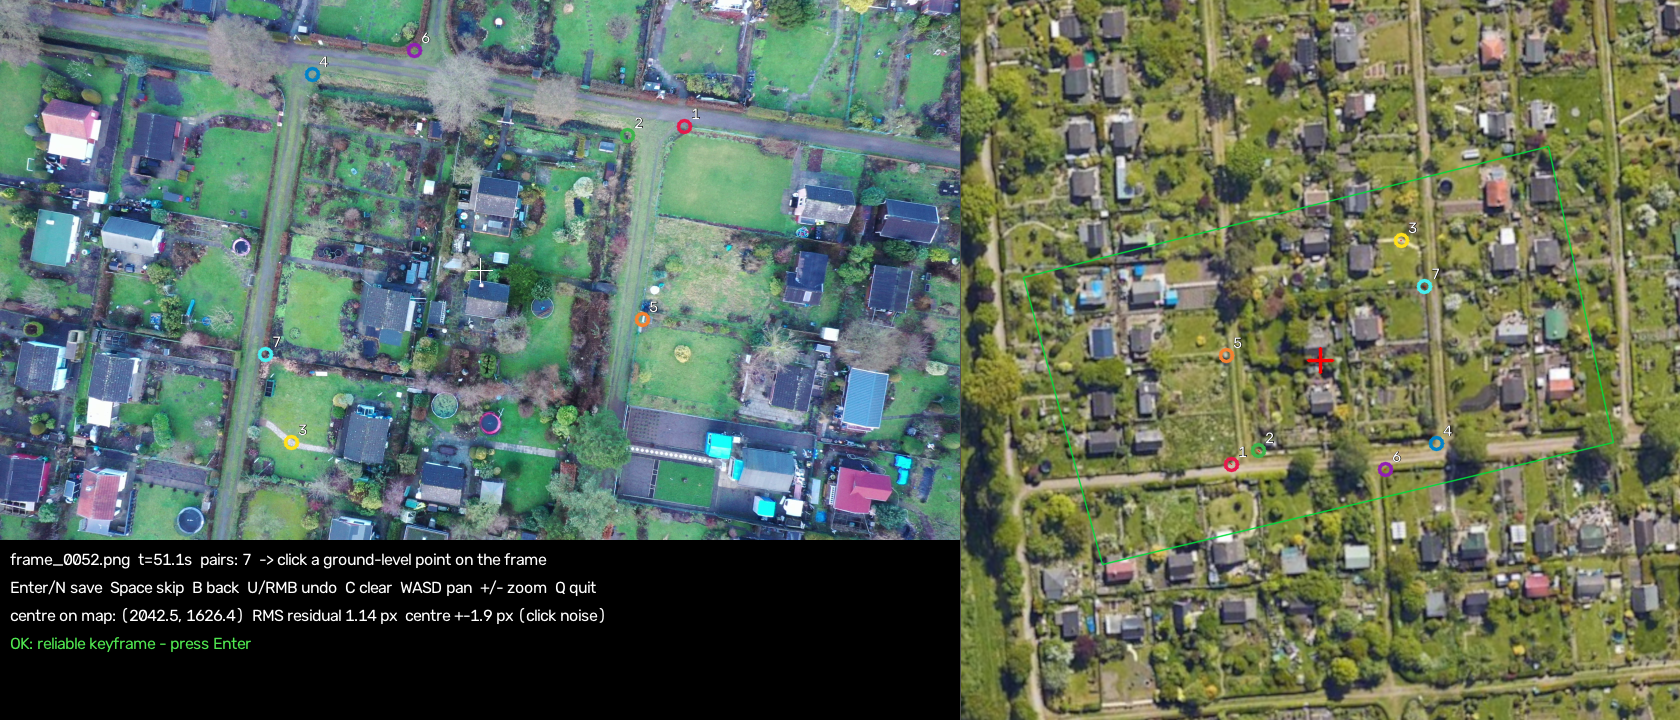
\includegraphics[width=\linewidth]{images/master/gt_annotation_example.png}
    \caption{Розмітка еталонного положення кадру 52 (кадр повернутий на $\approx 170^\circ$ відносно карти): пари точок пронумеровано, зеленим --- спроєктований контур кадру, червоним хрестиком --- центр кадру}
    \label{fig:gt-example}
\end{figure}

\textbf{Контроль якості розмітки.}\\
З чотирьох пар гомографія визначається точно, тому залишкова похибка дорівнює нулю й не дає змоги виявити помилку оператора. У першій версії розмітки саме такі кадри (по 4 пари, скупчені в одній частині кадру) давали <<похибку>> системи понад 100~\px{} для всіх методів одночасно. Тому опорний кадр вважається надійним, якщо:
\begin{enumerate}
    \item вказано не менше 5 пар;
    \item залишкова похибка кожної пари не перевищує 3~\px{}, інакше одна з точок хибна;
    \item 95-й процентиль зміщення центру за випадкового шуму кліків ($\sigma = 2$~пікселі кадру та 1~піксель карти, метод Монте-Карло) не перевищує 5~\px{}, інакше точки скупчені або центр кадру розташований далеко від них.
\end{enumerate}
Критерій не використовує результатів системи. Опорні кадри обрано візуально так, щоб на них були чіткі наземні орієнтири і щоб вони рівномірно покривали політ, включно з розворотами. Кадри над пустирем (33--40) і каналом (66--69) пропущено через відсутність надійних точок.

Розмічено 19 опорних кадрів, з них 18 надійних: 5--8 пар на кадр (у середньому 6,2), медіанна невизначеність центру 2,6~\px{} (максимум 5,0~\px{}), найбільша залишкова похибка пари --- 3,0~\px{}. Ненадійний кадр 40 (пустир, 4 пари) в метрики не включено. Для 7 надійних кадрів центр кадру лежить поза областю вказаних точок, тобто його положення екстрапольовано. Шум кліків цим критерієм враховано, але систематичні похибки (дисторсія ширококутного об'єктива, паралакс) за межами точок не оцінюються, що слід мати на увазі під час аналізу окремих кадрів.

Для кадрів між опорними еталон можна лінійно інтерполювати в часі, однак на розворотах інтерполяція <<зрізає>> траєкторію. Через це похибка за інтерпольованим еталоном вимірює насамперед похибку інтерполяції: для всіх чотирьох конфігурацій вона однакова, $\approx 38$~\px{}. Тому всі наведені нижче похибки обчислено лише за 18 надійними опорними кадрами.

\subsection{Зіставлення кадру з відомим фрагментом карти}
\label{sec:exp-pair}

\textbf{Результати для еталонної пари.}\\
Для перевірки конвеєра використано пару з курсової роботи: кадр 2 і фрагмент карти, що містить місце зйомки (результати --- у табл.~\ref{tab:pair}, приклади відповідностей --- на рис.~\ref{fig:pair}).

\begin{table}[H]
\centering
\caption{Зіставлення еталонної пари <<кадр 2 --- фрагмент 196>> (GPU, медіана часу з 5 запусків)}
\label{tab:pair}
\begin{tabular}{lcccccc}
\toprule
\textbf{Метод} & $N_{\text{all}}$ & $N_{\text{in}}$ & $r$ & $\bar{e}$, \px{} & масштаб $\sigma$ & час, с \\
\midrule
LightGlue & 310 & 89 & 0,29 & 1,58 & 0,267 & 0,25 \\
LoFTR & 631 & 184 & 0,29 & 1,40 & 0,202 & 0,27 \\
\bottomrule
\end{tabular}
\end{table}

\begin{figure}[H]
    \centering
    \begin{subfigure}{\linewidth}
        \centering
        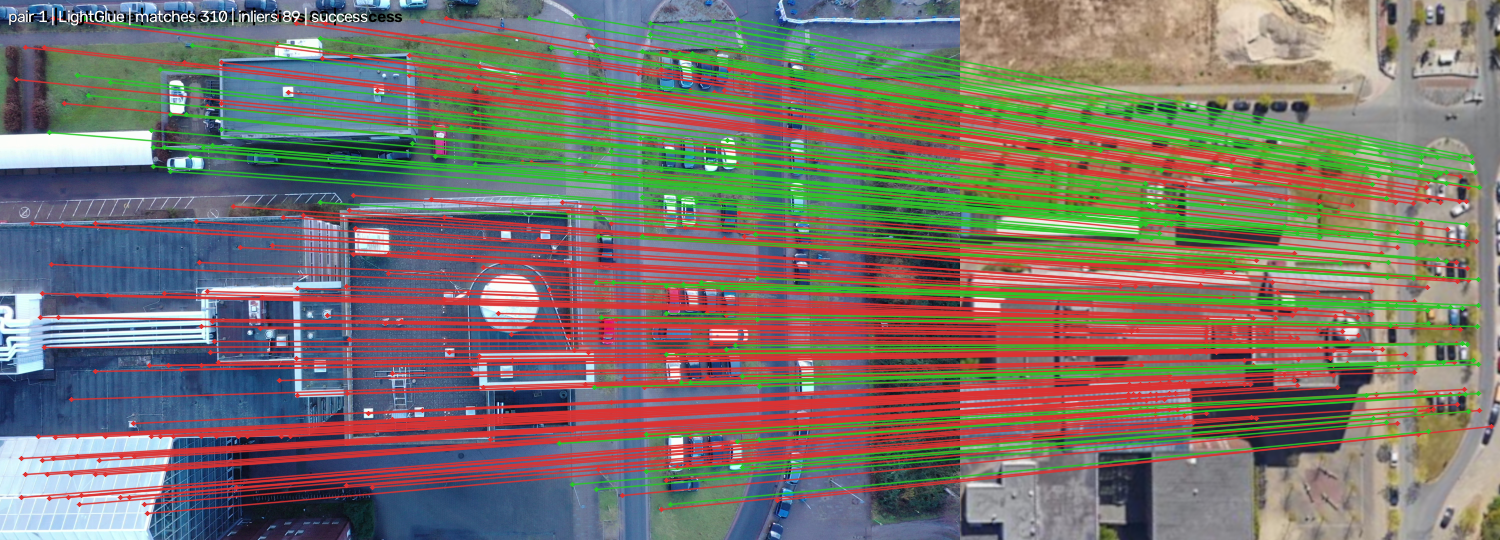
\includegraphics[width=0.92\linewidth]{images/master/pair_lightglue_matches.png}
        \caption{LightGlue}
    \end{subfigure}
    \vspace{2mm}
    \begin{subfigure}{\linewidth}
        \centering
        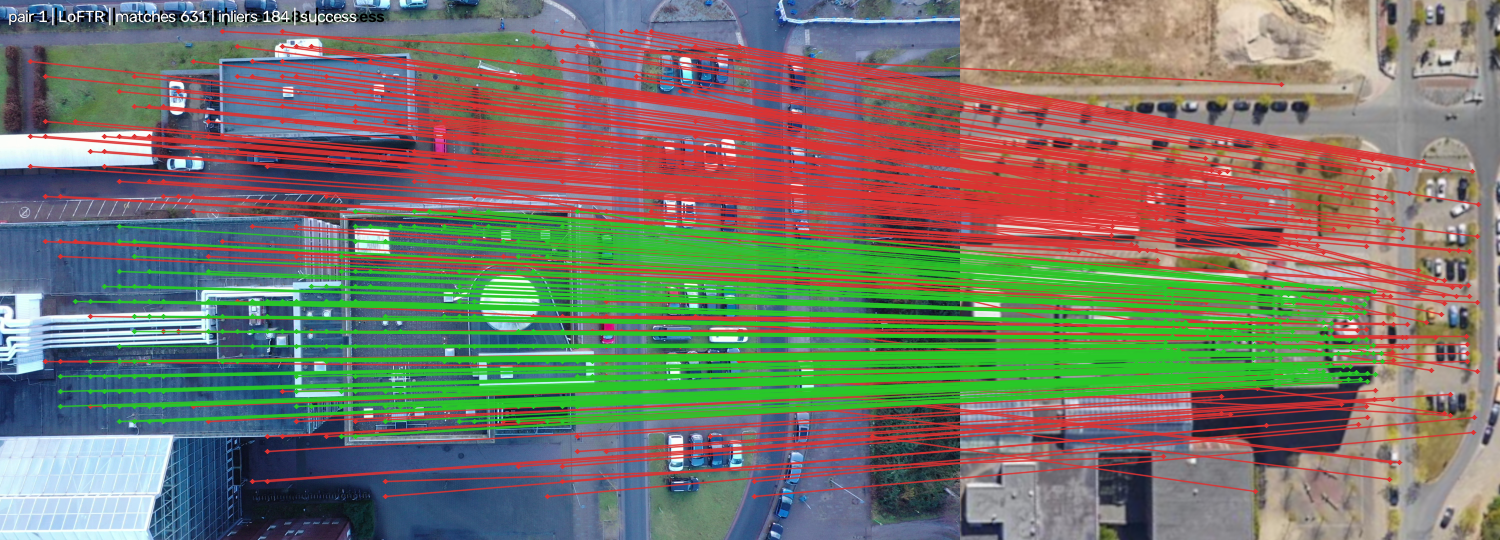
\includegraphics[width=0.92\linewidth]{images/master/pair_loftr_matches.png}
        \caption{LoFTR}
    \end{subfigure}
    \caption{Відповідності між кадром 2 (ліворуч) і фрагментом карти (праворуч): зеленим --- геометрично узгоджені, червоним --- відкинуті RANSAC}
    \label{fig:pair}
\end{figure}

\textbf{Виправлення методики курсової роботи.}\\
У курсовій роботі на цій парі LightGlue мав 229 геометрично узгоджених відповідностей проти 117 у LoFTR і працював повільніше (6,55~с проти 4,18~с). Аналіз прототипу показав, що ці результати отримано за нерівних умов. По-перше, SuperPoint неявно масштабував вхідні зображення до 1024~пікселів, тоді як LoFTR працював із 512. По-друге, обидва методи бачили лише центральну квадратну частину кадру, без нормалізації масштабу. По-третє, час вимірювався без прогрівання моделей. За однакових умов (табл.~\ref{tab:pair}) співвідношення змінюється: LoFTR знаходить удвічі більше геометрично узгоджених відповідностей за однакової їх частки, а час обробки пари на GPU для обох методів становить $\approx 0{,}25$~с. Тому числові результати курсової роботи надалі не використовуються.

\textbf{Калібрування масштабу кадру.}\\
Початкову оцінку $s_f \approx 0{,}25$ отримано вручну. Для її уточнення кадр 2 зіставлено з фрагментом карти $1024 \times 1024$, що повністю містить контур кадру. Обидва методи за обох оцінювачів і робочих масштабів $k \in \{1;\, 1{,}5\}$ дали узгоджений масштаб гомографії $\sigma = 0{,}267$--$0{,}277$, а оцінки центра кадру розійшлися не більше ніж на 16~\px{}. Отже, прийнято $s_f = 0{,}27$: кадр $1920 \times 1080$ покриває на карті ділянку $\approx 518 \times 292$~\px{}, ширшу за фрагмент 512~\px{}.

\textbf{Вплив непланарності сцени.}\\
На фрагменті 196 масштаб гомографії LoFTR ($\sigma = 0{,}20$) суттєво менший за калібрувальний (табл.~\ref{tab:pair}). Геометрично узгоджені відповідності LoFTR зосереджені на даху високої будівлі, ближчому до камери, ніж земля, тому RANSAC оцінює гомографію площини даху, а не площини землі (рис.~\ref{fig:pair}б). Центр кадру при цьому все одно визначається з похибкою $\approx 15$~\px{}, оскільки він сам розташований на цьому даху. Цей ефект є прямим наслідком припущення про плоску сцену.

\textbf{Контрольна перевірка на хибних фрагментах.}\\
Кадр 2 зіставлено з 33 фрагментами, серед яких є як сусідні до місця зйомки, так і віддалені. Фрагменти, що не перетинаються з кадром, дали щонайбільше 15 (LightGlue) і 14 (LoFTR) геометрично узгоджених відповідностей і всі були відкинуті: частина за порогом $N_{\text{in}} \ge 15$, частина --- перевіркою правдоподібності гомографії. Усі фрагменти, що перетинаються з кадром, дали від 18 до 240 таких відповідностей і пройшли перевірку. Запас між цими групами невеликий, тому для вибору фрагмента додатково використовуються частка відповідностей і умова потрапляння центра кадру у фрагмент (п.~\ref{sec:search}).

\subsection{Автоматичний пошук фрагмента для одиночного кадру}

Для кадру 2 виконано пошук без будь-якої інформації про місце зйомки (табл.~\ref{tab:search}, рис.~\ref{fig:global-loc}).

\begin{table}[H]
\centering
\caption{Автоматичний пошук фрагмента для кадру 2}
\label{tab:search}
\small
\begin{tabular}{lccccc}
\toprule
\textbf{Запуск} & \textbf{Перевірено} & \textbf{Пройшли фільтр} & \textbf{Переможець} & \textbf{Центр $(X, Y)$, \px{}} & \textbf{Час, с} \\
\midrule
LightGlue, уся карта, кеш & 384 & 5 & 220 & (1121,4;\ 2344,7) & 33 \\
LoFTR, обмежена область & 56 & 5 & 197 & (1108,6;\ 2327,5) & 18 \\
LoFTR, кожен 2-й рядок і стовпець & 96 & 1 & 197 & (1108,6;\ 2327,5) & 32 \\
\bottomrule
\end{tabular}
\end{table}

\begin{figure}[H]
    \centering
    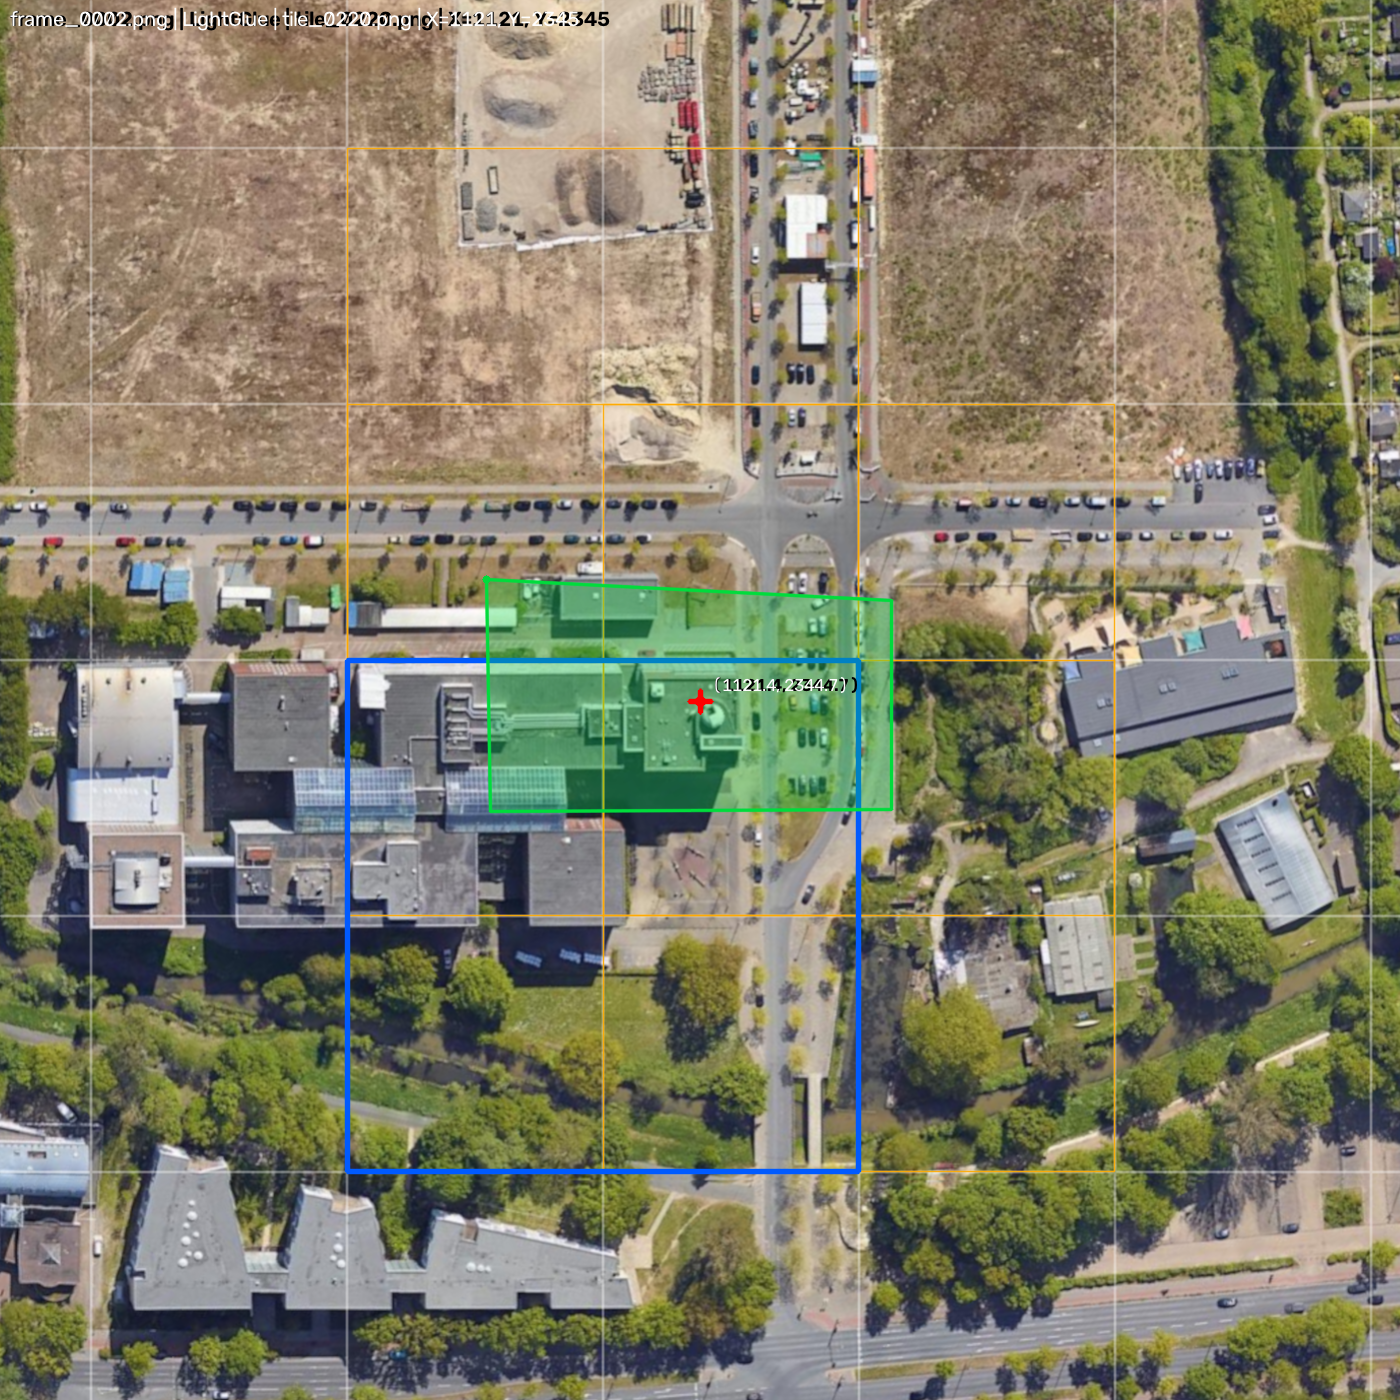
\includegraphics[width=0.75\linewidth]{images/master/global_loc_zoom.png}
    \caption{Результат автоматичного пошуку для кадру 2: сітка перевірених фрагментів, фрагменти, що пройшли фільтр (помаранчеві), фрагмент-переможець (синій), контур огляду камери (зелений) і центр кадру (червоний)}
    \label{fig:global-loc}
\end{figure}

В обох випадках переможцем став фрагмент, суміжний з еталонним фрагментом 196, який також містить центр кадру. Оцінка LoFTR відрізняється від калібрувальної оцінки $\approx(1110;\ 2330)$ на $\approx 3$~\px{}, оцінка LightGlue --- на $\approx 19$~\px{}. Усі фрагменти, що пройшли фільтр, перетинаються з місцем зйомки; жоден віддалений фрагмент фільтр не пройшов. Перегляд усієї карти з кешем ознак займає 33~с (85~мс на фрагмент), що прийнятно для початкової ініціалізації, але не для обробки кожного кадру. Це обґрунтовує використання трекера.

\subsection{Локалізація послідовності кадрів і вплив компенсації курсу}
\label{sec:exp-yaw}

Траєкторія польоту являє собою облітання кварталу: на північ, схід, південь і захід. Під час польоту курс змінюється приблизно так: $0^\circ \to 90^\circ \to 175^\circ \to -90^\circ \to -40^\circ$. Щоб оцінити внесок компенсації курсу, трекер (LightGlue + RANSAC) запущено на всіх 95 кадрах з компенсацією та без неї (табл.~\ref{tab:yaw}, рис.~\ref{fig:yaw}).

\begin{table}[H]
\centering
\caption{Вплив компенсації курсу на трекінг послідовності (LightGlue + RANSAC, 95 кадрів)}
\label{tab:yaw}
\begin{tabular}{lcc}
\toprule
& \textbf{Без компенсації} & \textbf{З компенсацією} \\
\midrule
\textsc{initialized} / \textsc{tracking} / \textsc{interpolated} / \textsc{lost} & 1 / 17 / 3 / 74 & 1 / 94 / 0 / 0 \\
Супровід утрачено & на кадрі 19, не відновлено & ні \\
Загальний час обробки & $\approx 41$~хв & 133~с \\
\bottomrule
\end{tabular}
\end{table}

\begin{figure}[H]
    \centering
    \begin{subfigure}{0.49\linewidth}
        \centering
        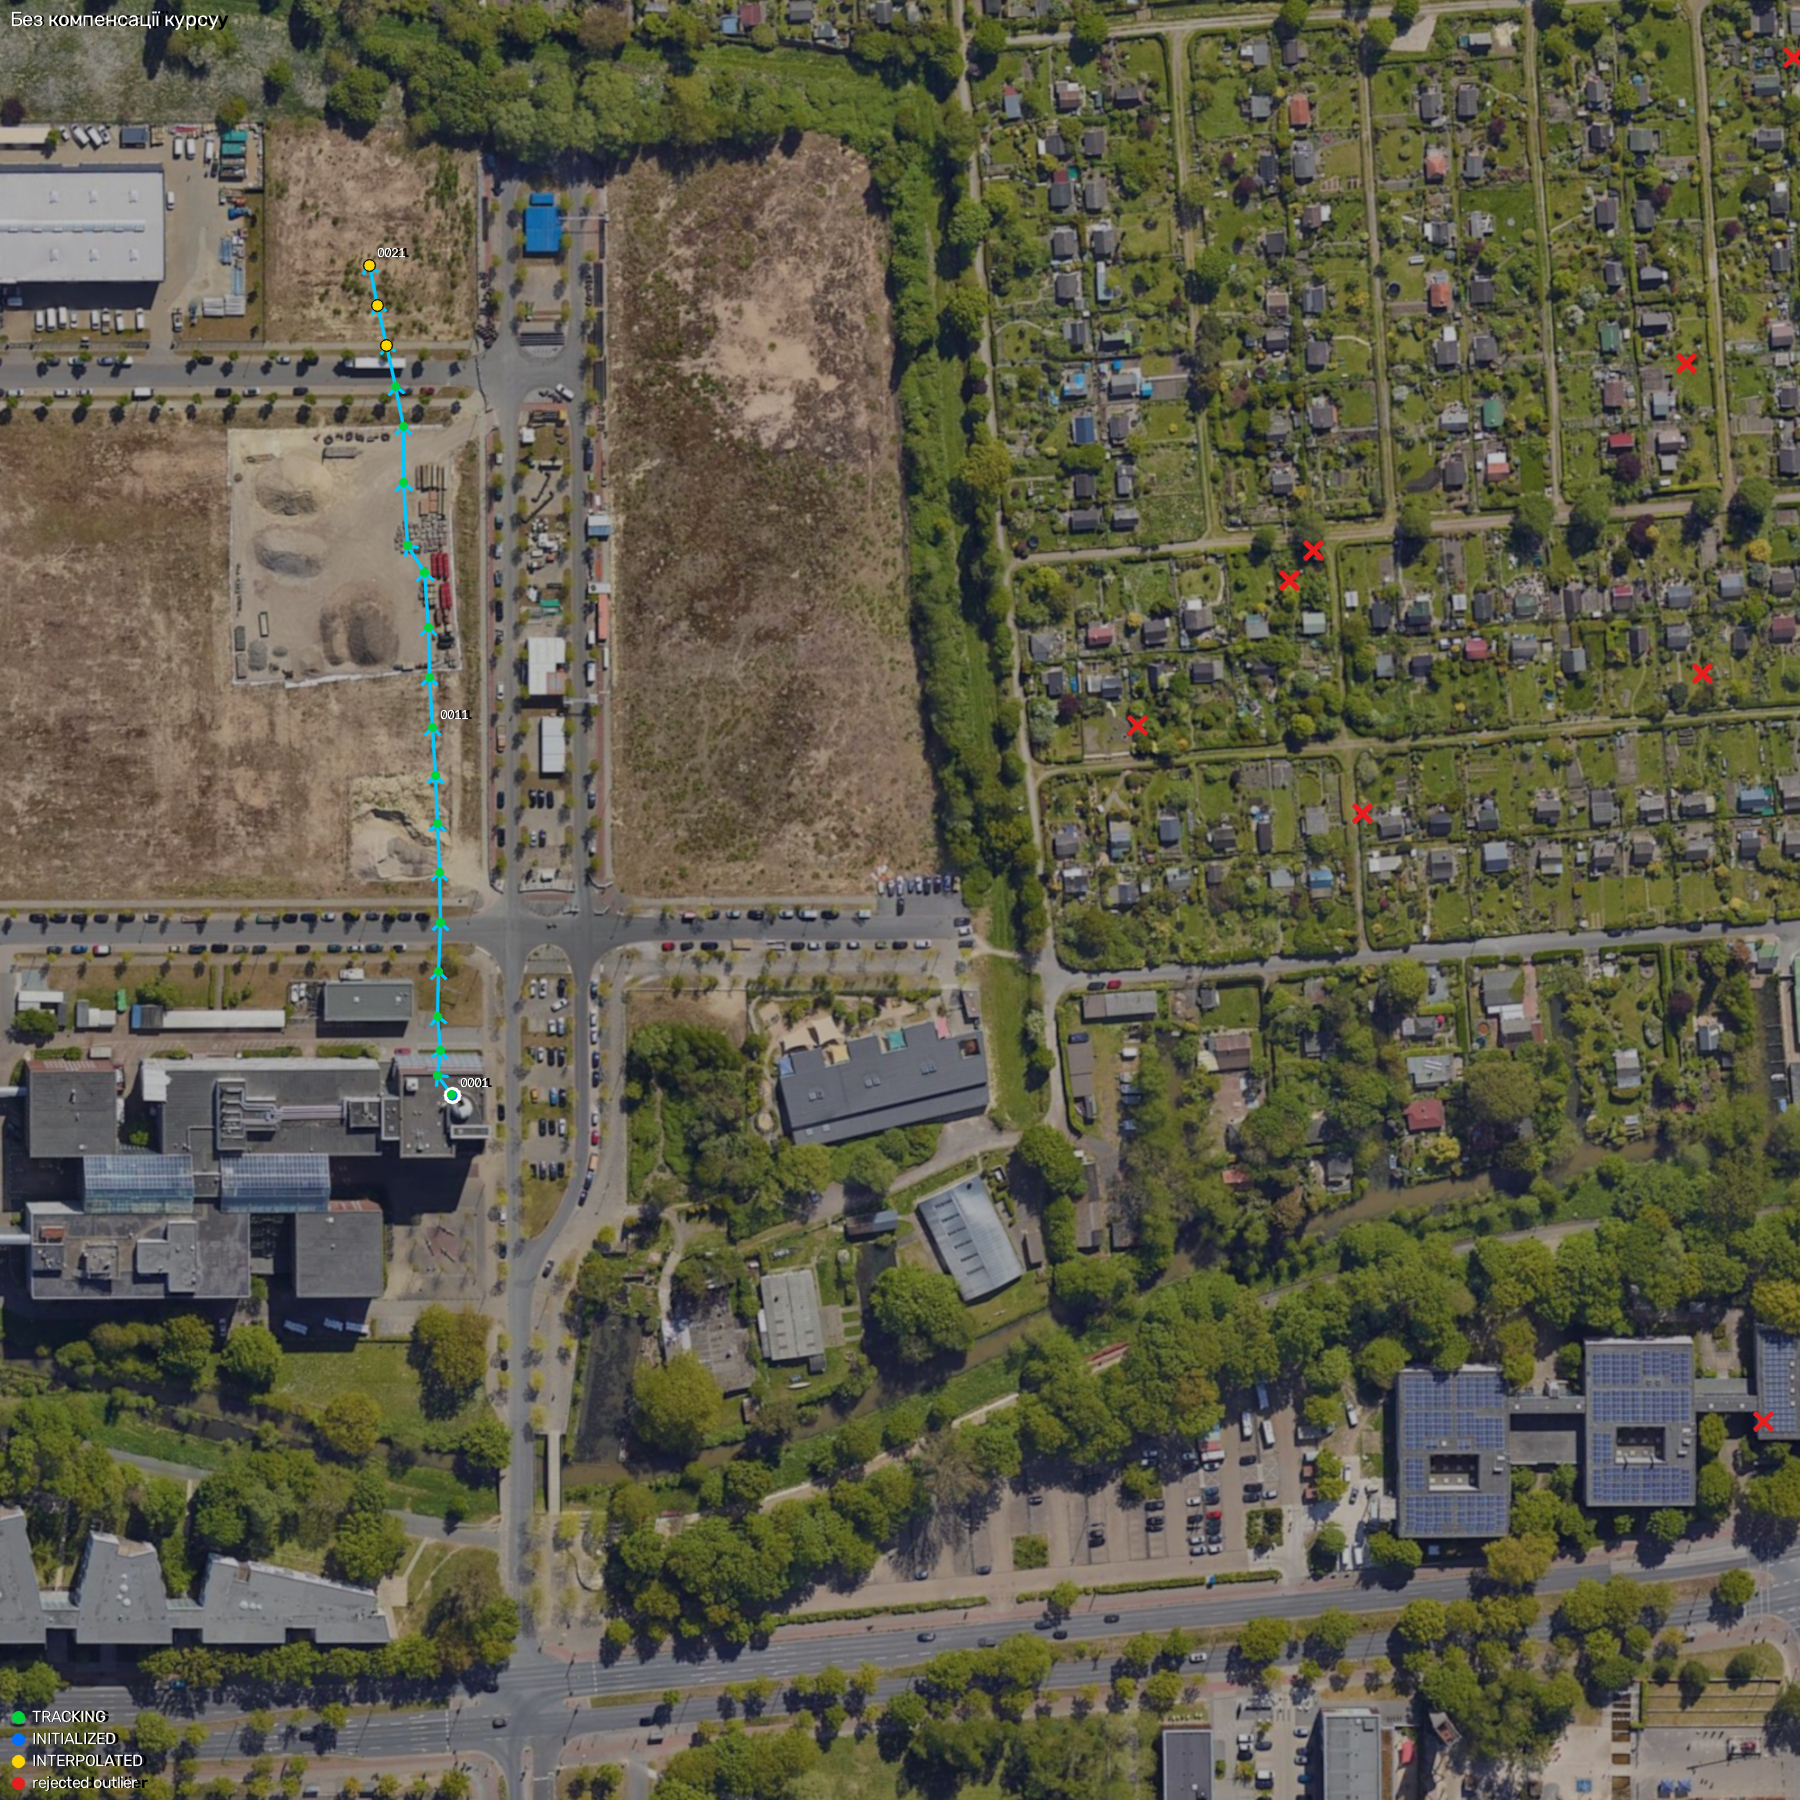
\includegraphics[width=\linewidth]{images/master/trajectory_no_yaw.png}
        \caption{без компенсації курсу}
    \end{subfigure}
    \hfill
    \begin{subfigure}{0.49\linewidth}
        \centering
        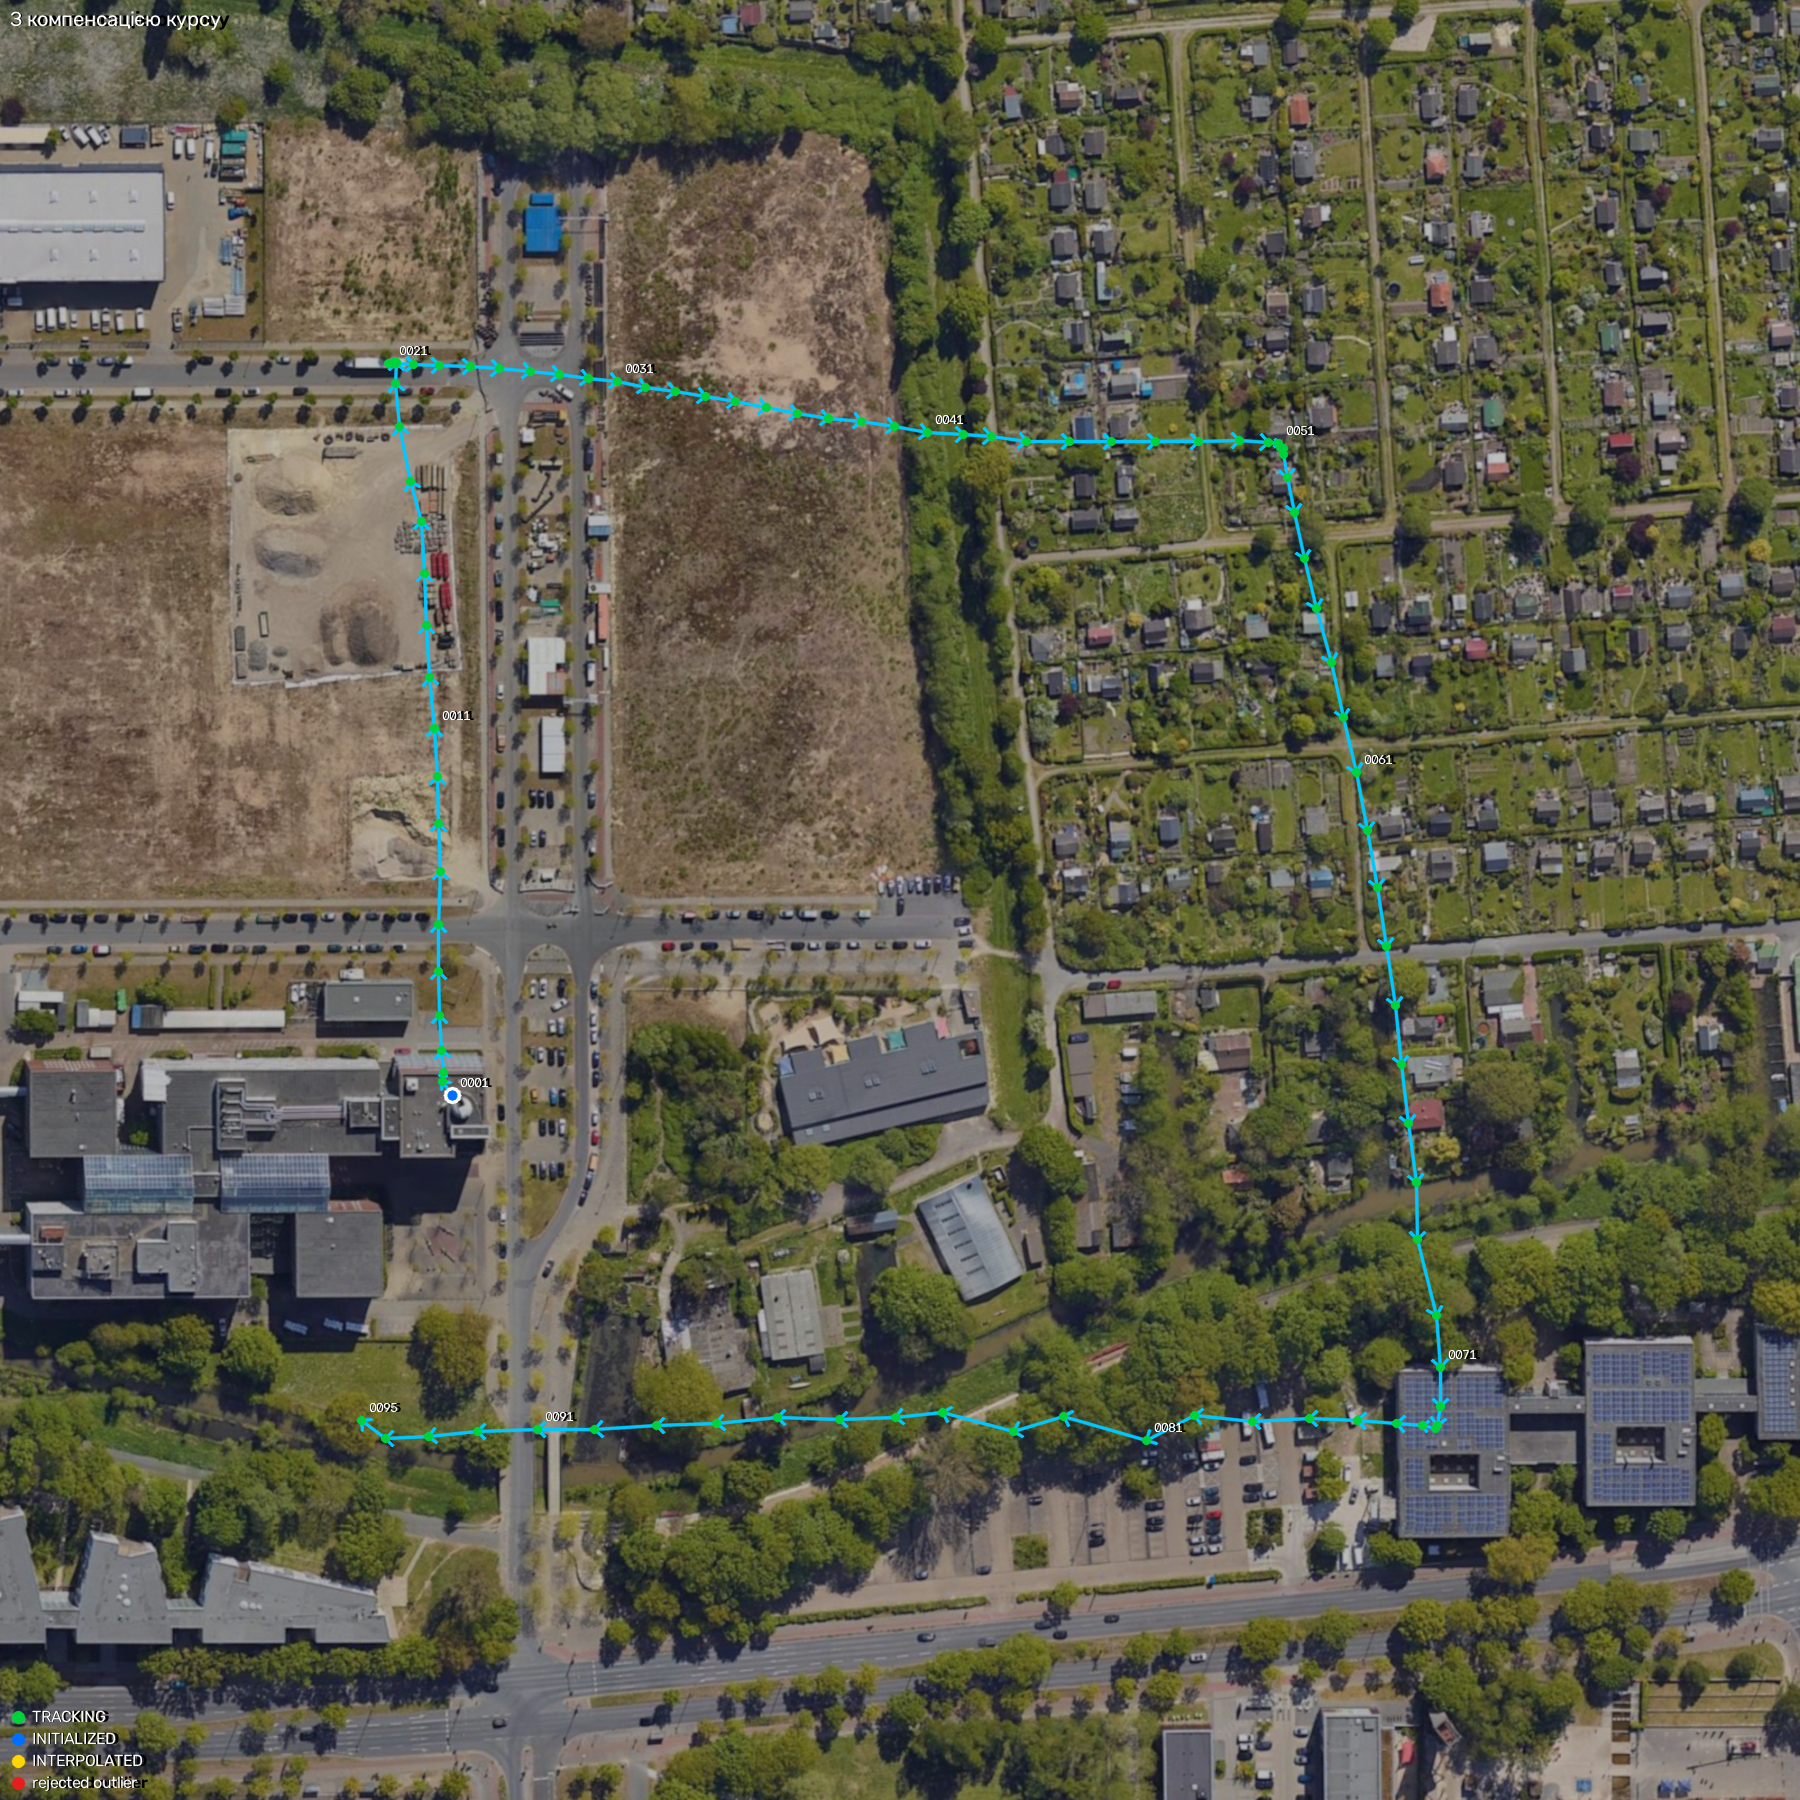
\includegraphics[width=\linewidth]{images/master/trajectory_with_yaw.png}
        \caption{з компенсацією курсу}
    \end{subfigure}
    \caption{Траєкторія, відновлена трекером: зелені точки --- \textsc{tracking}, жовті --- \textsc{interpolated}, червоні хрестики --- кандидати, відкинуті через низький бал або кінематичну перевірку}
    \label{fig:yaw}
\end{figure}

Без компенсації трекер утрачає супровід на першому розвороті (кадр 19, поворот кадру $\approx 50^\circ$). Глобальний пошук із курсом $0^\circ$ після цього вже не знаходить відповідного фрагмента. Кожен кадр у стані \textsc{lost} займає $\approx 32$~с, тому загальний час обробки зростає до 41~хв. З компенсацією всі чотири розвороти відстежено лише за прогнозом курсу; перебір додаткових гіпотез курсу знадобився для одного кадру. Компенсація курсу виявилася необхідною умовою роботи системи на реальному польоті.

\subsection{Порівняння методів LightGlue і LoFTR}
\label{sec:exp-methods}

Усі чотири конфігурації відстежили всю послідовність: 94 кадри зі статусом \textsc{tracking} і один \textsc{initialized}, лише для LightGlue + MAGSAC++ один кадр екстрапольовано. Кінематична перевірка жодного разу не відкинула оцінку, а повторна глобальна ініціалізація не знадобилася. Показники трекінгу та точності наведено в табл.~\ref{tab:tracking} і \ref{tab:accuracy}; відновлені траєкторії разом з еталоном --- на рис.~\ref{fig:traj-gt}, похибки на опорних кадрах --- на рис.~\ref{fig:error}.

\begin{table}[H]
\centering
\caption{Показники трекінгу послідовності з 95 кадрів}
\label{tab:tracking}
\small
\begin{tabular}{lcccccc}
\toprule
\multirow{2}{*}{\textbf{Конфігурація}} & \multicolumn{2}{c}{\textbf{Час кадру, с}} & \textbf{Глобальний} & \multirow{2}{*}{\textbf{Медіана} $N_{\text{in}}$} & \multirow{2}{*}{$\bar{r}$} & \multirow{2}{*}{$\bar{e}$, \px{}} \\
& середній & $P_{90}$ & \textbf{пошук, с} & & & \\
\midrule
LightGlue + RANSAC & 1,08 & 1,40 & 38,3 & 81 & 0,48 & 1,65 \\
LightGlue + MAGSAC++ & 0,78 & 1,02 & 20,1 & 87 & 0,50 & 1,73 \\
LoFTR + RANSAC & 2,72 & 2,93 & 127,9 & 316 & 0,59 & 1,27 \\
LoFTR + MAGSAC++ & 2,27 & 2,49 & 87,5 & 353 & 0,61 & 1,33 \\
\bottomrule
\end{tabular}
\end{table}

\begin{table}[H]
\centering
\caption{Похибка локалізації на 18 надійних опорних кадрах, \px{}}
\label{tab:accuracy}
\small
\begin{tabular}{lccccccc}
\toprule
\textbf{Конфігурація} & \textbf{Середня} & \textbf{Медіана} & \textbf{RMSE} & $P_{90}$ & \textbf{Макс.} & \textbf{S@10} & \textbf{S@25} \\
\midrule
LightGlue + RANSAC & 7,2 & 6,0 & 9,5 & 16,8 & 22,9 & 83\,\% & 100\,\% \\
LightGlue + MAGSAC++ & 7,5 & 5,7 & 10,2 & 16,5 & 27,5 & 78\,\% & 94\,\% \\
LoFTR + RANSAC & 4,9 & 3,1 & 7,3 & 9,0 & 24,2 & 94\,\% & 100\,\% \\
LoFTR + MAGSAC++ & 5,2 & 2,9 & 8,9 & 8,2 & 33,2 & 94\,\% & 94\,\% \\
\bottomrule
\end{tabular}
\end{table}

\begin{figure}[H]
    \centering
    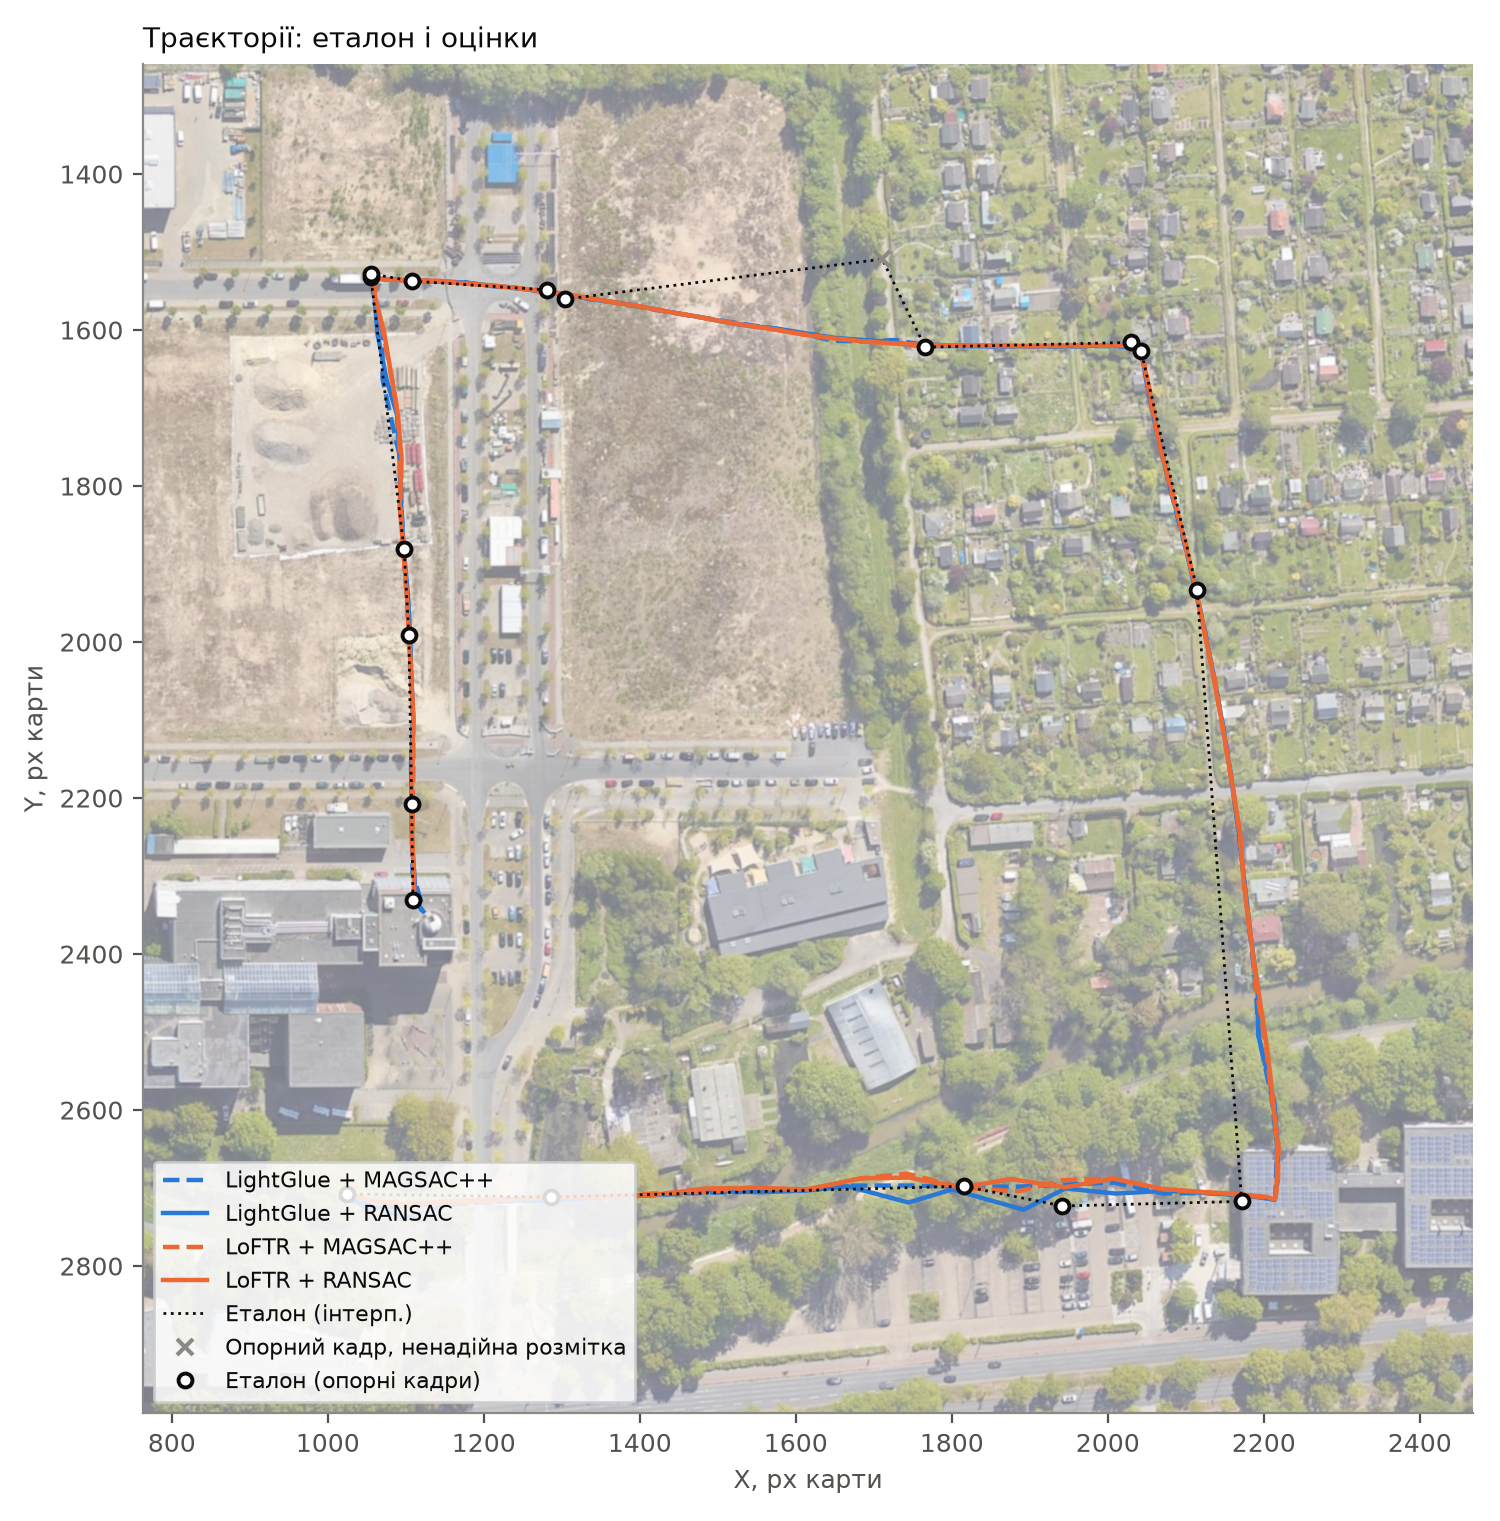
\includegraphics[width=0.8\linewidth]{images/master/trajectories_vs_gt.png}
    \caption{Траєкторії, відновлені чотирма конфігураціями, та еталонні положення опорних кадрів}
    \label{fig:traj-gt}
\end{figure}

\begin{figure}[H]
    \centering
    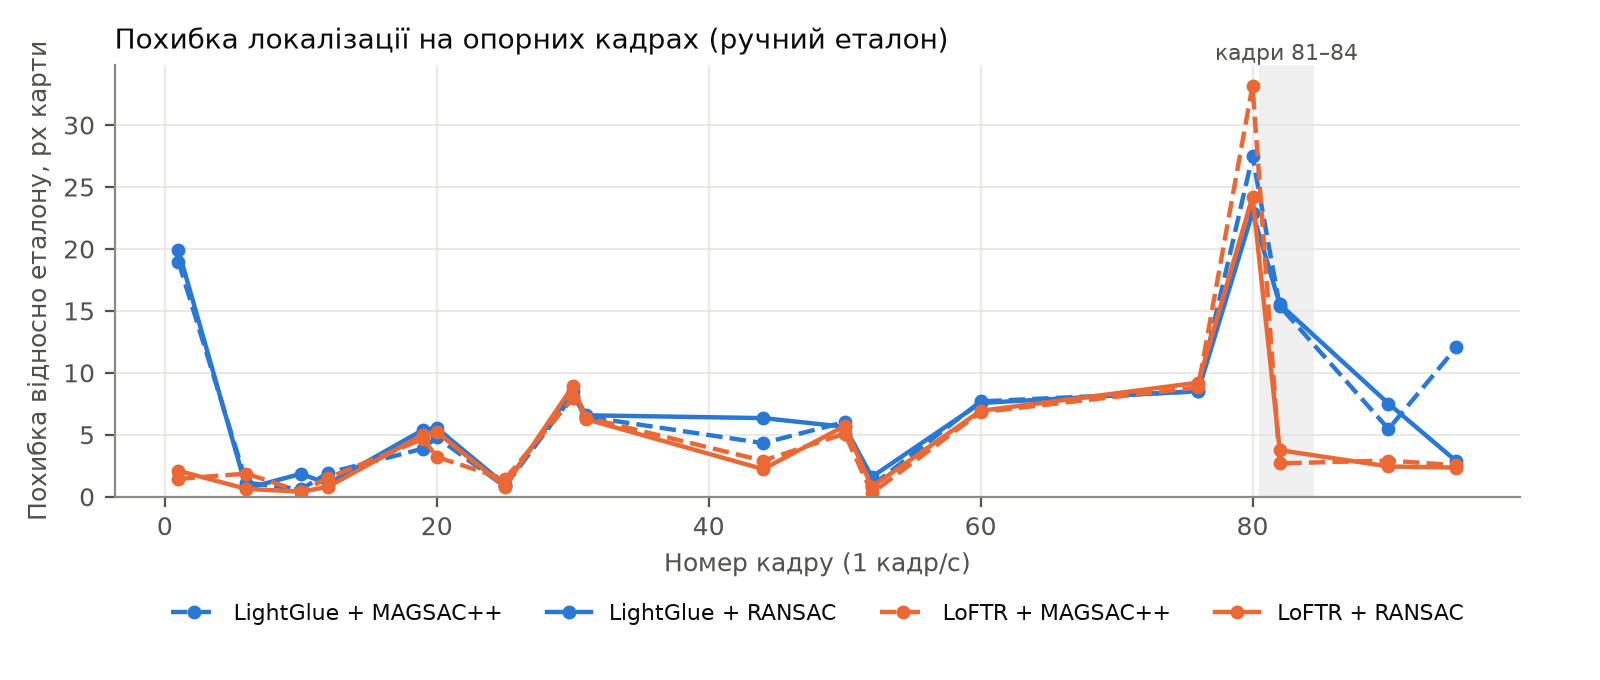
\includegraphics[width=\linewidth]{images/master/error_over_time.png}
    \caption{Похибка локалізації на опорних кадрах уздовж польоту}
    \label{fig:error}
\end{figure}

\textbf{Точність.}\\
LoFTR забезпечує меншу медіанну похибку, ніж LightGlue: $\approx 3$~\px{} проти $\approx 6$~\px{}. Частка кадрів із похибкою не більше 10~\px{} становить 94\,\% проти 78--83\,\%. У парному порівнянні з однаковим оцінювачем RANSAC LoFTR точніший на 14 з 18 опорних кадрів (знаковий тест, $p = 0{,}031$), з MAGSAC++ --- на 13 з 18 ($p = 0{,}096$). На більшості кадрів різниця між методами не перевищує 1--2~\px{}, тобто є порівнянною з невизначеністю еталона. Перевагу LoFTR формують насамперед кілька складних кадрів:
\begin{itemize}
    \item кадр 1: 19,9~\px{} у LightGlue проти 2,1~\px{} у LoFTR --- LightGlue під час ініціалізації оцінює гомографію площини даху високої будівлі (див. п.~\ref{sec:exp-pair});
    \item кадр 82 поблизу масиву дерев: 15,5~\px{} проти 3,8~\px{};
    \item кадр 90: 7,5~\px{} проти 2,4~\px{}.
\end{itemize}

На кадрі 80 усі чотири конфігурації мають близьку похибку 23--33~\px{}. Збіг похибки незалежних методів вказує на систематичну причину, спільну для всіх. Найімовірніше, це неточність еталона: усі точки розмітки цього кадру розташовані в його лівій третині (дорога й паркінг), права частина кадру зайнята деревами, а центр кадру екстрапольовано. Без кадру 80 середня похибка становить 6,2--6,3~\px{} для LightGlue і 3,6--3,7~\px{} для LoFTR; максимальна похибка LoFTR зменшується до 9,2~\px{}.

\textbf{Кількість відповідностей і швидкодія.}\\
LoFTR знаходить у 3,6--4 рази більше геометрично узгоджених відповідностей (медіана 316--353 проти 81--87) з більшою їх часткою та меншою похибкою репроєкції. Водночас LoFTR у 2,5--2,9 раза повільніший у режимі трекінгу (2,3--2,7~с проти 0,8--1,1~с на кадр) і в 3,3 (RANSAC) та 4,4 (MAGSAC++) раза повільніший під час глобального пошуку, оскільки для нього неможливе кешування ознак фрагментів. Між собою траєкторії конфігурацій відрізняються з медіаною 0,8--1,7~\px{}; найбільші розбіжності (19--43~\px{}) припадають на кадри 79--83 над деревами.

\subsection{Порівняння оцінювачів RANSAC і MAGSAC++}

Розподіл часу обробки кадру в режимі трекінгу наведено на рисунку~\ref{fig:timing}.

\begin{figure}[H]
    \centering
    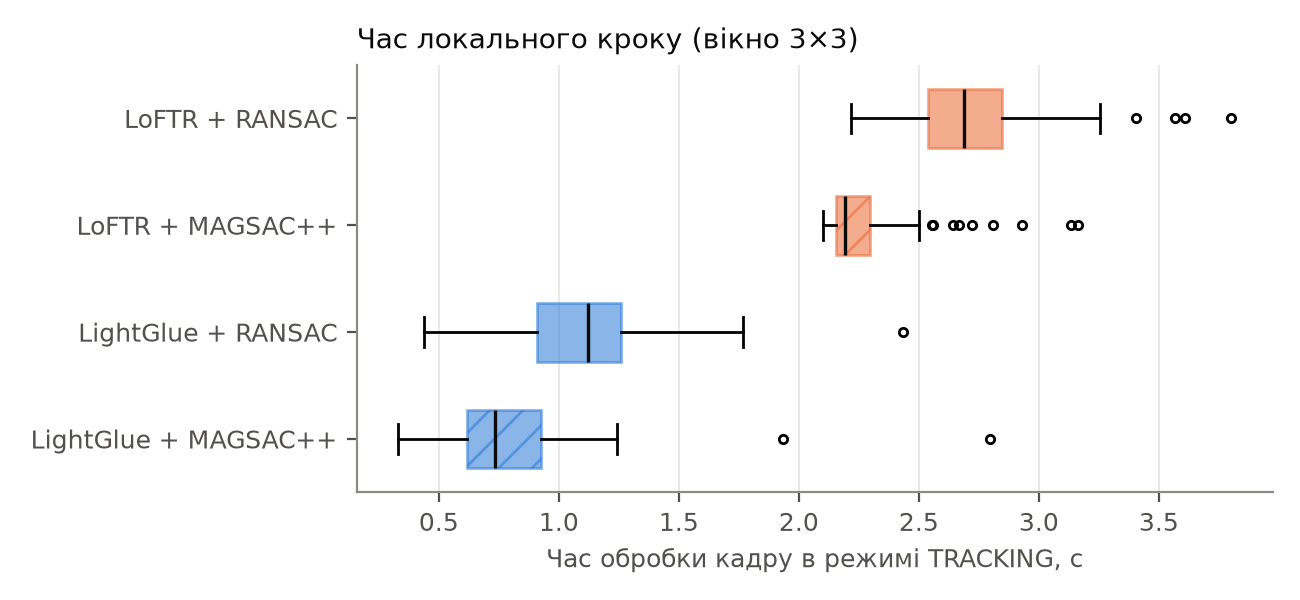
\includegraphics[width=0.75\linewidth]{images/master/timing_local.png}
    \caption{Час обробки кадру в режимі \textsc{tracking} для чотирьох конфігурацій}
    \label{fig:timing}
\end{figure}

Заміна RANSAC на MAGSAC++ скорочує час кадру на 28\,\% для LightGlue (1,08 $\to$ 0,78~с) і на 17\,\% для LoFTR (2,72 $\to$ 2,27~с), а час глобального пошуку --- у 1,9 і 1,5 раза відповідно. Виграш отримано насамперед на фрагментах, які не містять місця зйомки: на таких фрагментах реалізація RANSAC в OpenCV не може достроково зупинитися і виконує всі 5000 ітерацій, тоді як MAGSAC++ завершується за кілька мілісекунд.

Статистично значущої різниці в точності не виявлено. У парному порівнянні MAGSAC++ точніший за RANSAC на 12 з 18 кадрів для LightGlue ($p = 0{,}24$) і на 9 з 18 для LoFTR ($p = 1{,}0$), медіанна різниця не перевищує 0,2~\px{}. Траєкторії, отримані з різними оцінювачами, відрізняються з медіаною 1,2~\px{} (LightGlue) і 0,8~\px{} (LoFTR). Таким чином, MAGSAC++ дає змогу пришвидшити систему без втрати точності. Конфігурація LightGlue + MAGSAC++ --- єдина, що забезпечує обробку кадру не довше 1~с (середнє 0,78~с, $P_{90}$ 1,02~с).

\subsection{Стійкість до спотворень зображення}
\label{sec:exp-robust}

Для 19 кадрів (кожен п'ятий кадр послідовності) штучно застосовано спотворення до оригінального кадру $1920 \times 1080$:
\begin{itemize}
    \item зниження яскравості $I' = \alpha I$;
    \item зниження контрасту $I' = \alpha (I - \mu) + \mu$, де $\mu$ --- середнє значення каналу;
    \item адитивний гауссів шум;
    \item лінійне розмиття руху;
    \item поворот кадру без компенсації;
    \item помилка у заданому масштабі $s_f$.
\end{itemize}
Пул фрагментів і компенсація курсу були такими самими, як у трекері на відповідному кадрі. Для кожного кадру обчислено відношення $N_{\text{in}}$ до значення для неспотвореного кадру та зміщення знайденого центру. Результати наведено в табл.~\ref{tab:robust} і на рис.~\ref{fig:robust}.

\begin{table}[H]
\centering
\caption{Стійкість до спотворень (19 кадрів): частка локалізованих кадрів і медіанне відношення $N_{\text{in}} / N_{\text{in}}^{\text{без спотв.}}$}
\label{tab:robust}
\small
\begin{tabular}{lcccc}
\toprule
\multirow{2}{*}{\textbf{Спотворення}} & \multicolumn{2}{c}{\textbf{LightGlue}} & \multicolumn{2}{c}{\textbf{LoFTR}} \\
\cmidrule(lr){2-3}\cmidrule(lr){4-5}
& локалізовано & відношення & локалізовано & відношення \\
\midrule
яскравість $\alpha = 0{,}7$ / $0{,}5$ & 100 / 100\,\% & 1,00 / 1,01 & 100 / 100\,\% & 0,97 / 0,97 \\
контраст $\alpha = 0{,}7$ / $0{,}5$ & 100 / 100\,\% & 1,02 / 0,99 & 100 / 100\,\% & 1,00 / 0,97 \\
шум $\sigma = 10$ / $25$ & 95 / 95\,\% & 0,99 / 0,92 & 100 / 95\,\% & 1,02 / 0,95 \\
розмиття 5 / 9 пікселів & 100 / 100\,\% & 1,02 / 1,02 & 100 / 100\,\% & 1,02 / 1,04 \\
поворот $15^\circ$ / $30^\circ$ & 95 / 95\,\% & 1,03 / 0,99 & 95 / 95\,\% & 0,82 / 0,52 \\
поворот $45^\circ$ & 53\,\% & 0,35 & 11\,\% & 0 \\
поворот $90^\circ$ & 0\,\% & 0 & 0\,\% & 0 \\
масштаб $\times 0{,}8$ / $\times 1{,}25$ & 100 / 95\,\% & 0,68 / 1,29 & 100 / 100\,\% & 0,71 / 1,05 \\
\bottomrule
\end{tabular}
\end{table}

\begin{figure}[H]
    \centering
    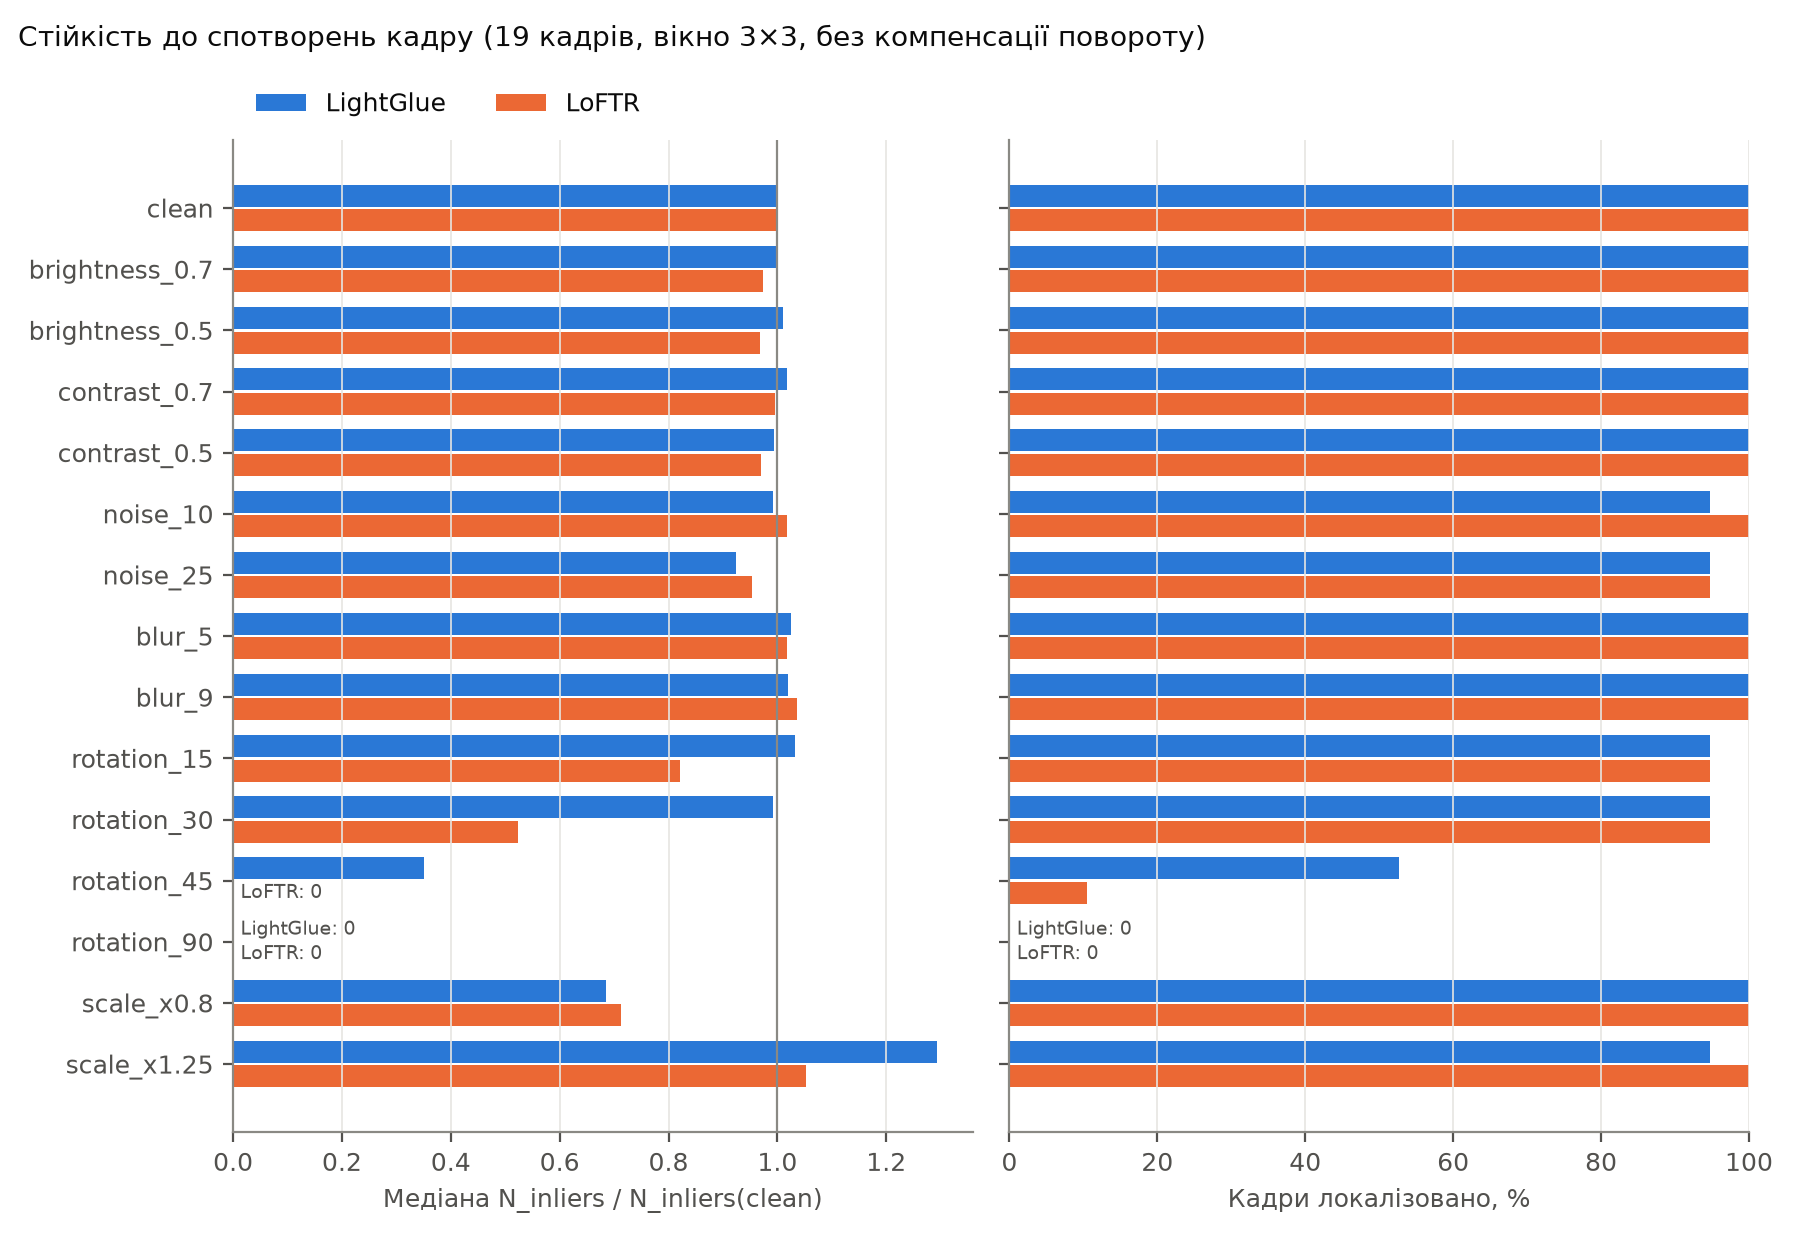
\includegraphics[width=\linewidth]{images/master/robustness.png}
    \caption{Стійкість методів до спотворень кадру}
    \label{fig:robust}
\end{figure}

Зміни яскравості й контрасту, гауссів шум і розмиття в досліджених межах практично не впливають на результат: кількість геометрично узгоджених відповідностей зберігається, а медіанне зміщення центру не перевищує 1,5~\px{}. Слабкий вплив розмиття частково пояснюється тим, що після масштабування кадру з коефіцієнтом 0,27 ядро 9 пікселів зменшується до $\approx 2{,}4$ пікселя.

Визначальним чинником виявився поворот кадру. LightGlue зберігає працездатність до $30^\circ$, а LoFTR втрачає половину відповідностей уже при $30^\circ$. При $45^\circ$ локалізовано лише 53\,\% (LightGlue) і 11\,\% (LoFTR) кадрів, при $90^\circ$ --- жодного. Ці результати кількісно обґрунтовують компенсацію курсу, описану в п.~\ref{sec:tracking}. Похибка масштабу на 20--25\,\% не призводить до втрати локалізації, але зменшення заданого масштабу на 20\,\% скорочує кількість відповідностей приблизно на 30\,\%.

\subsection{Аналіз проблемних ділянок місцевості}

Для кожного кадру за контуром огляду обчислено дві ознаки ділянки ортофотоплану:
\begin{itemize}
    \item частку рослинності за індексом Excess Green $\text{ExG} = 2g - r - b$ у хроматичних координатах \cite{exg} (піксель вважається рослинністю, якщо $\text{ExG} > 0{,}05$);
    \item текстурованість --- середній модуль градієнта Собеля яскравості.
\end{itemize}
Залежність кількості геометрично узгоджених відповідностей від номера кадру та частки рослинності наведено на рисунку~\ref{fig:terrain}, кореляції --- у табл.~\ref{tab:terrain}.

\begin{figure}[H]
    \centering
    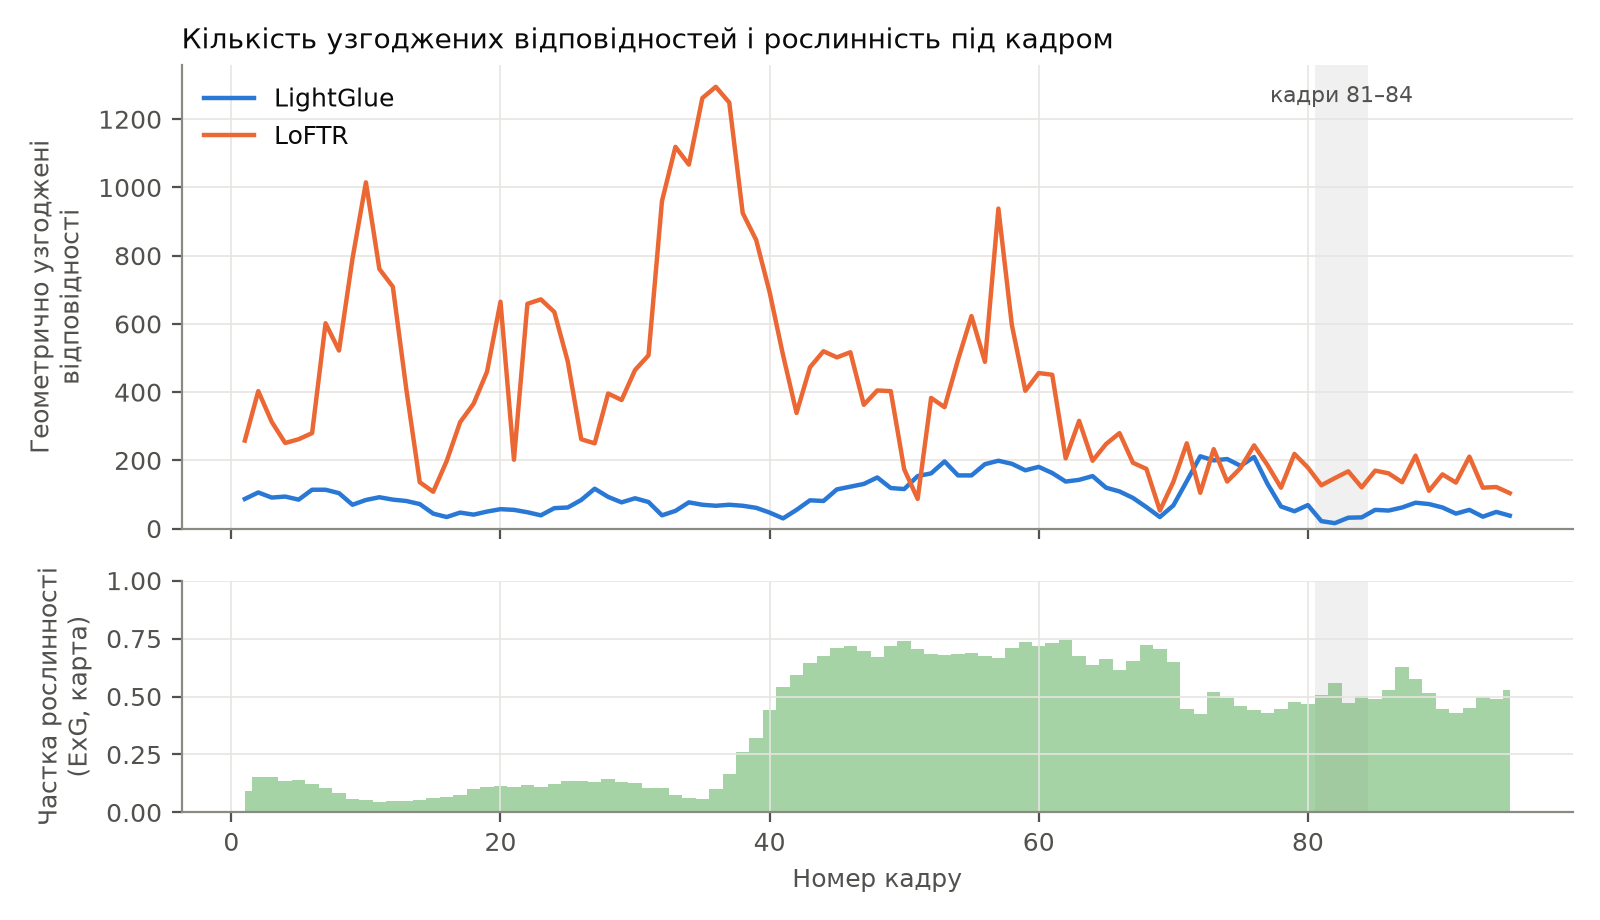
\includegraphics[width=\linewidth]{images/master/inliers_vs_terrain.png}
    \caption{Кількість геометрично узгоджених відповідностей уздовж польоту (вгорі) і частка рослинності під кадром (внизу); сірим виділено кадри 81--84}
    \label{fig:terrain}
\end{figure}

\begin{table}[H]
\centering
\caption{Зв'язок кількості геометрично узгоджених відповідностей з ознаками місцевості (кореляція Спірмена $\rho$, RANSAC)}
\label{tab:terrain}
\begin{tabular}{lcccc}
\toprule
\textbf{Метод} & $\rho$ (рослинність) & $\rho$ (текстура) & \textbf{Медіана} $N_{\text{in}}$, кадри 81--84 & \textbf{Медіана} $N_{\text{in}}$, усі \\
\midrule
LightGlue & $+0{,}37$ & $+0{,}65$ & 27 & 81 \\
LoFTR & $-0{,}29$ & $+0{,}29$ & 138 & 316 \\
\bottomrule
\end{tabular}
\end{table}

На ділянці кадрів 81--84 (паркінг і канал, оточені деревами) кількість геометрично узгоджених відповідностей падає втричі для LightGlue і вдвічі для LoFTR. Саме тут методи найбільше розходяться між собою. Водночас частка рослинності під кадром сама по собі не пояснює це падіння: для LightGlue кореляція з нею навіть додатна, оскільки дачні ділянки з будівлями мають високу частку рослинності, але багаті на деталі. Кращим предиктором для LightGlue є текстурованість ($\rho = 0{,}65$); для LoFTR зв'язок з обома ознаками слабкий. Імовірною причиною падіння на кадрах 81--84 є сезонна різниця крон листяних дерев (на відео --- без листя, на карті --- з листям), однак підтвердження цієї гіпотези потребує окремого дослідження.

% TODO: експерименти з розміром фрагмента (256/512/768/1024) і часткою перекриття (25/50 %),
%       передбачені технічним завданням, ще не проведено. Після їх виконання додати
%       підрозділ з результатами (див. обмеження нижче щодо розміру фрагмента 512).

\subsection{Обмеження розробленої системи}

Під час експериментів виявлено такі обмеження:
\begin{itemize}
    \item \textbf{Плоска модель сцени.} Гомографія описує лише площину. Високі будівлі спричиняють паралакс, і RANSAC може оцінити площину даху замість площини землі (кадр 1 у LightGlue, кадр 2 у LoFTR).
    \item \textbf{Розмір фрагмента.} Контур огляду кадру ($\approx 518 \times 292$~\px{}) ширший за фрагмент 512~\px{}, тому жоден фрагмент не містить кадр повністю.
    \item \textbf{Фіксований масштаб.} Масштаб кадру $s_f$ відкалібровано на одному кадрі, і він вважається сталим. Під час польоту оцінений масштаб гомографії змінювався в межах 0,20--0,32 (медіана 0,269), проте в трекері він не уточнюється.
    \item \textbf{Чутливість до повороту.} Без компенсації курсу обидва методи непрацездатні при повороті кадру на $45^\circ$ і більше; перший глобальний пошук виконується з курсом $0^\circ$.
    \item \textbf{Швидкодія.} Повний перебір карти займає 20--128~с залежно від конфігурації. Обмеження 1~с на кадр у режимі трекінгу на використаному GPU виконує лише LightGlue + MAGSAC++.
    \item \textbf{Одиниці вимірювання.} Без просторової прив'язки ортофотоплану похибки визначено в пікселях карти; переведення в метри потребує відомого розміру пікселя.
    \item \textbf{Обсяг даних і еталона.} Дослідження виконано на одному польоті (95 кадрів) і 18 опорних кадрах. Опорні кадри обрано за наявністю наземних орієнтирів, тому міські ділянки в еталоні представлені ширше, ніж у польоті загалом.
\end{itemize}

\subsection{Висновки за результатами експериментів}

\begin{enumerate}
    \item Розроблена система автоматично знаходить відповідний фрагмент ортофотоплану для кадру БпЛА без апріорної інформації про місце зйомки та відновлює траєкторію польоту. На послідовності з 95 кадрів усі чотири конфігурації локалізували кожен кадр без втрати супроводу.
    \item Медіанна похибка локалізації на опорних кадрах становить $\approx 3$~\px{} для LoFTR і $\approx 6$~\px{} для LightGlue; не більше ніж 10~\px{} помиляється 94\,\% і 78--83\,\% кадрів відповідно. LoFTR точніший на більшості кадрів, і його перевага найпомітніша на складних ділянках (дах високої будівлі, дерева).
    \item LightGlue у 2,5--2,9 раза швидший за LoFTR у режимі трекінгу і допускає кешування ознак карти. Конфігурація LightGlue + MAGSAC++ --- єдина, що обробляє кадр не довше 1~с (0,78~с у середньому).
    \item MAGSAC++ скорочує час обробки на 17--28\,\% без статистично значущої зміни точності, тому його доцільно використовувати замість класичного RANSAC.
    \item Обидва методи стійкі до змін яскравості, контрасту, шуму та помірного розмиття, але не до повороту кадру понад $30$--$45^\circ$. Компенсація курсу за оцінкою кута з гомографії попередніх кадрів виявилася необхідною: без неї супровід утрачається на першому розвороті.
    \item Результати курсової роботи щодо переваги LightGlue за кількістю відповідностей отримано за нерівних умов (різний масштаб вхідних зображень). За однакових умов LoFTR знаходить більше геометрично узгоджених відповідностей.
    \item Вибір методу визначається вимогами застосування: LoFTR --- для вищої точності, LightGlue + MAGSAC++ --- для обробки в реальному часі на обмеженому обладнанні.
\end{enumerate}

% =============================================================================
\providecommand{\px}{пкс}
\providecommand{\code}[1]{\texttt{#1}}

\newpage
\section{Результати експериментів та їх оцінка}
\label{sec:experiments}

\subsection{Методика експериментального дослідження}

\textbf{Дані та обладнання.}\\
Усі експерименти виконано на даних, описаних у розділі~\ref{sec:implementation}: ортофотоплан $6200 \times 4320$~пікселів, розбитий на 384 фрагменти $512 \times 512$ з перекриттям 50\,\%, і 95 кадрів відео польоту БпЛА з частотою 1~кадр/с. Обчислення виконано на GPU NVIDIA GeForce GTX 1650. Якщо не зазначено інше, використано параметри за замовчуванням: $s_f = 0{,}27$, $k = 1$, поріг RANSAC 3~\px{}, мінімум 15 геометрично узгоджених відповідностей.

\textbf{Досліджувані конфігурації.}\\
Порівнювалися чотири конфігурації системи --- поєднання методу зіставлення (LightGlue або LoFTR) та оцінювача гомографії (RANSAC або MAGSAC++). Решта етапів (масштабування, геометрична перевірка, фільтр і ранжування, трекер, компенсація курсу) для всіх конфігурацій однакові. Це забезпечує коректність порівняння: на відміну від курсової роботи, обидва методи отримують зображення однакового масштабу.

\textbf{Метрики зіставлення.}\\
Для пари <<кадр --- фрагмент>> використовуються:
\begin{itemize}
    \item $N_{\text{all}}$ --- кількість відповідностей, які повернув метод;
    \item $N_{\text{in}}$ --- кількість геометрично узгоджених відповідностей (похибка репроєкції не більша за поріг RANSAC);
    \item $r = N_{\text{in}} / N_{\text{all}}$ --- частка геометрично узгоджених відповідностей;
    \item $\bar{e}$ --- середня похибка репроєкції геометрично узгоджених відповідностей, \px{}. За побудовою вона не перевищує порогу RANSAC, тому характеризує точність відповідностей, а не успішність локалізації;
    \item час обробки, с.
\end{itemize}

\textbf{Метрики локалізації.}\\
Похибка локалізації кадру $i$ визначається відносно еталонного положення (п.~\ref{sec:gt}):
\begin{equation}
E_i = \sqrt{(X_i - X_i^{\text{ет}})^2 + (Y_i - Y_i^{\text{ет}})^2}, \quad \text{\px{}}.
\end{equation}
За сукупністю кадрів обчислюються середня, медіанна та максимальна похибка, середньоквадратична похибка $\text{RMSE} = \sqrt{\tfrac{1}{N}\sum_i E_i^2}$, 90-й процентиль $P_{90}$, а також частка успішних локалізацій
\begin{equation}
\text{Success@}K = \frac{\left|\{ i : E_i \le K \}\right|}{N}, \qquad K \in \{10, 25, 50\}~\text{\px{}},
\end{equation}
де $N$ --- кількість усіх кадрів з еталоном; кадри, для яких система не видала положення, вважаються неуспішними. Ортофотоплан не має просторової прив'язки, тому похибки наведено в пікселях карти і в метри не переводяться.

\subsection{Еталонні координати}
\label{sec:gt}

Для обчислення похибки локалізації потрібне еталонне положення кадру, незалежне від системи, що оцінюється. Використання як еталона результатів самої системи або їхнього візуального <<уточнення>> призвело б до заниженої оцінки похибки, тому еталон побудовано за ручними відповідностями точок.

\textbf{Процедура розмітки.}\\
Для опорного кадру оператор у спеціально розробленому інструменті вказує щонайменше 5 пар відповідних точок <<кадр $\leftrightarrow$ карта>>, розташованих на рівні землі (кути дорожньої розмітки та бордюрів, перехрестя доріжок, основи стовпів). Дахи будівель не використовуються, оскільки через паралакс вони зміщені відносно земної поверхні. За всіма парами методом найменших квадратів (без RANSAC) оцінюється гомографія $H_{\text{ет}}$, і центр кадру переноситься на карту. Приклад розмітки наведено на рисунку~\ref{fig:gt-example}.

\begin{figure}[H]
    \centering
    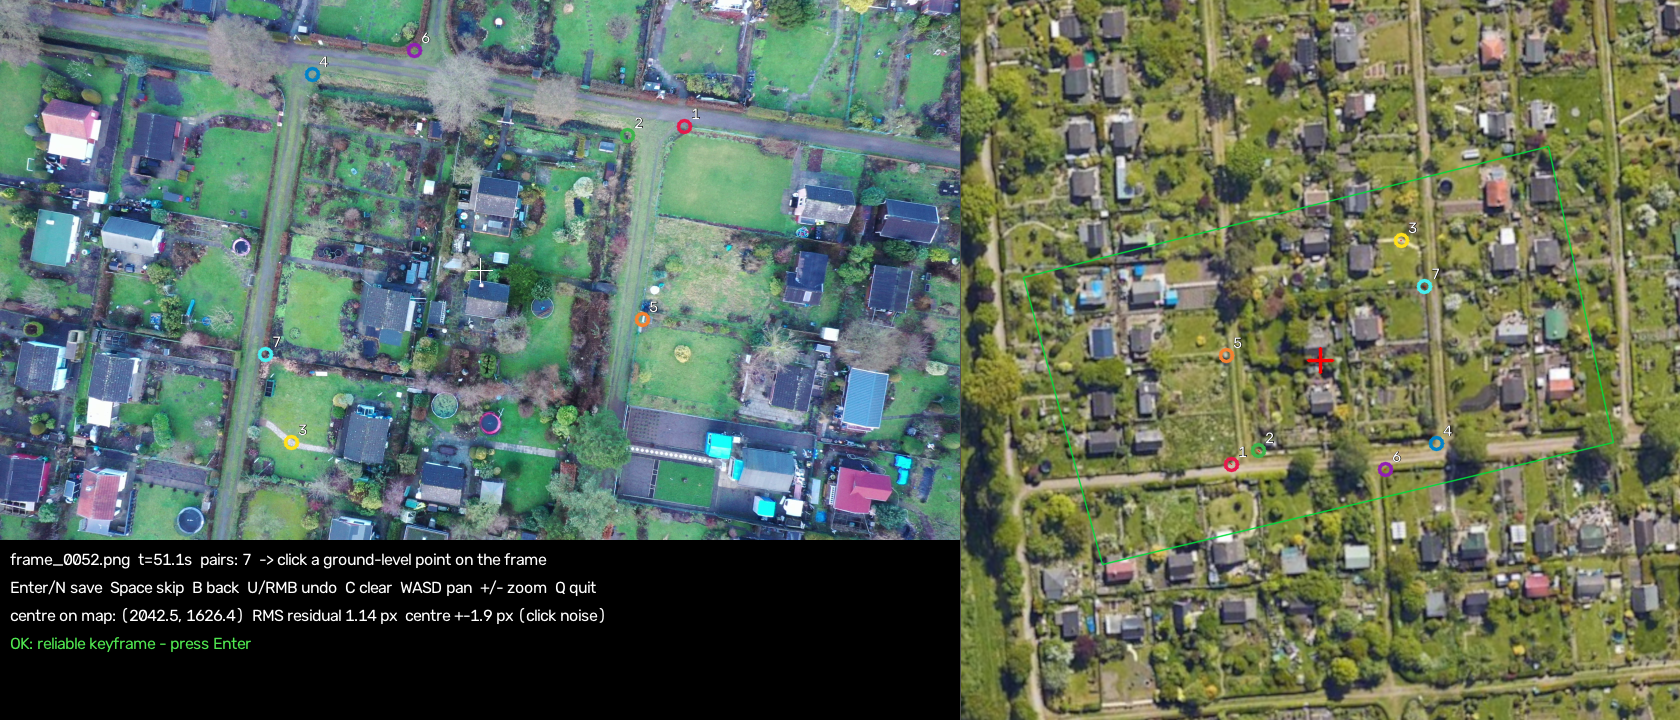
\includegraphics[width=\linewidth]{images/master/gt_annotation_example.png}
    \caption{Розмітка еталонного положення кадру 52 (кадр повернутий на $\approx 170^\circ$ відносно карти): пари точок пронумеровано, зеленим --- спроєктований контур кадру, червоним хрестиком --- центр кадру}
    \label{fig:gt-example}
\end{figure}

\textbf{Контроль якості розмітки.}\\
З чотирьох пар гомографія визначається точно, тому залишкова похибка дорівнює нулю й не дає змоги виявити помилку оператора. У першій версії розмітки саме такі кадри (по 4 пари, скупчені в одній частині кадру) давали <<похибку>> системи понад 100~\px{} для всіх методів одночасно. Тому опорний кадр вважається надійним, якщо:
\begin{enumerate}
    \item вказано не менше 5 пар;
    \item залишкова похибка кожної пари не перевищує 3~\px{}, інакше одна з точок хибна;
    \item 95-й процентиль зміщення центру за випадкового шуму кліків ($\sigma = 2$~пікселі кадру та 1~піксель карти, метод Монте-Карло) не перевищує 5~\px{}, інакше точки скупчені або центр кадру розташований далеко від них.
\end{enumerate}
Критерій не використовує результатів системи. Опорні кадри обрано візуально так, щоб на них були чіткі наземні орієнтири і щоб вони рівномірно покривали політ, включно з розворотами. Кадри над пустирем (33--40) і каналом (66--69) пропущено через відсутність надійних точок.

Розмічено 19 опорних кадрів, з них 18 надійних: 5--8 пар на кадр (у середньому 6,2), медіанна невизначеність центру 2,6~\px{} (максимум 5,0~\px{}), найбільша залишкова похибка пари --- 3,0~\px{}. Ненадійний кадр 40 (пустир, 4 пари) в метрики не включено. Для 7 надійних кадрів центр кадру лежить поза областю вказаних точок, тобто його положення екстрапольовано. Шум кліків цим критерієм враховано, але систематичні похибки (дисторсія ширококутного об'єктива, паралакс) за межами точок не оцінюються, що слід мати на увазі під час аналізу окремих кадрів.

Для кадрів між опорними еталон можна лінійно інтерполювати в часі, однак на розворотах інтерполяція <<зрізає>> траєкторію. Через це похибка за інтерпольованим еталоном вимірює насамперед похибку інтерполяції: для всіх чотирьох конфігурацій вона однакова, $\approx 38$~\px{}. Тому всі наведені нижче похибки обчислено лише за 18 надійними опорними кадрами.

\subsection{Зіставлення кадру з відомим фрагментом карти}
\label{sec:exp-pair}

\textbf{Результати для еталонної пари.}\\
Для перевірки конвеєра використано пару з курсової роботи: кадр 2 і фрагмент карти, що містить місце зйомки (результати --- у табл.~\ref{tab:pair}, приклади відповідностей --- на рис.~\ref{fig:pair}).

\begin{table}[H]
\centering
\caption{Зіставлення еталонної пари <<кадр 2 --- фрагмент 196>> (GPU, медіана часу з 5 запусків)}
\label{tab:pair}
\begin{tabular}{lcccccc}
\toprule
\textbf{Метод} & $N_{\text{all}}$ & $N_{\text{in}}$ & $r$ & $\bar{e}$, \px{} & масштаб $\sigma$ & час, с \\
\midrule
LightGlue & 310 & 89 & 0,29 & 1,58 & 0,267 & 0,25 \\
LoFTR & 631 & 184 & 0,29 & 1,40 & 0,202 & 0,27 \\
\bottomrule
\end{tabular}
\end{table}

\begin{figure}[H]
    \centering
    \begin{subfigure}{\linewidth}
        \centering
        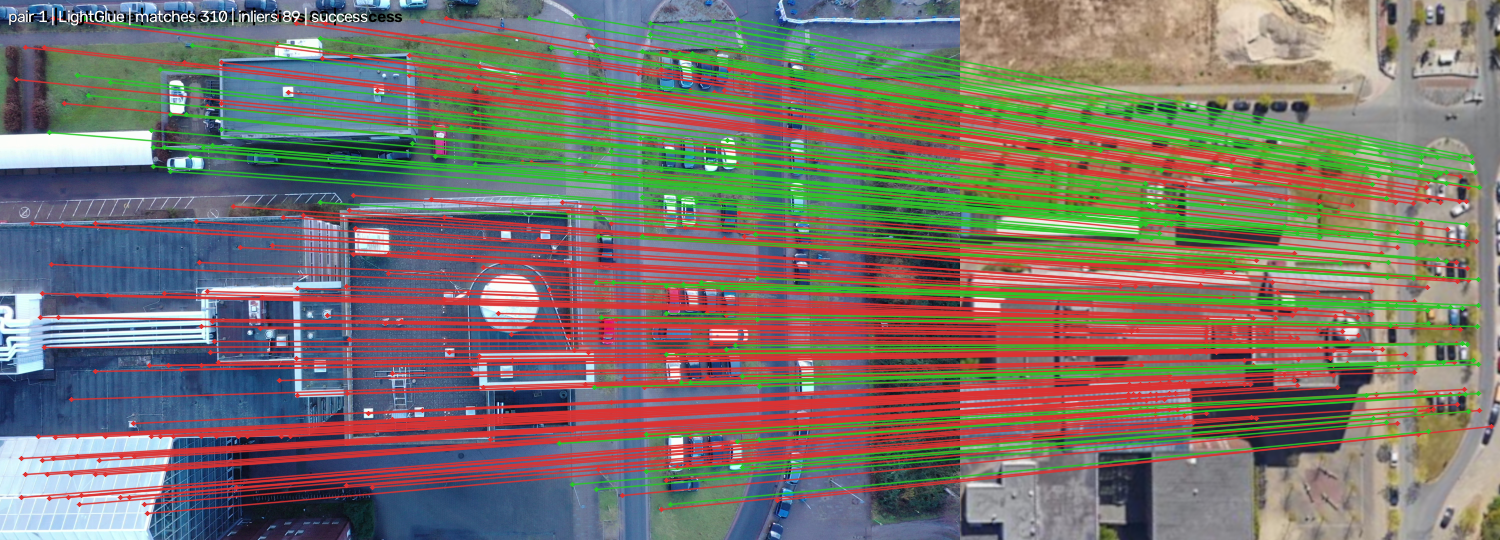
\includegraphics[width=0.92\linewidth]{images/master/pair_lightglue_matches.png}
        \caption{LightGlue}
    \end{subfigure}
    \vspace{2mm}
    \begin{subfigure}{\linewidth}
        \centering
        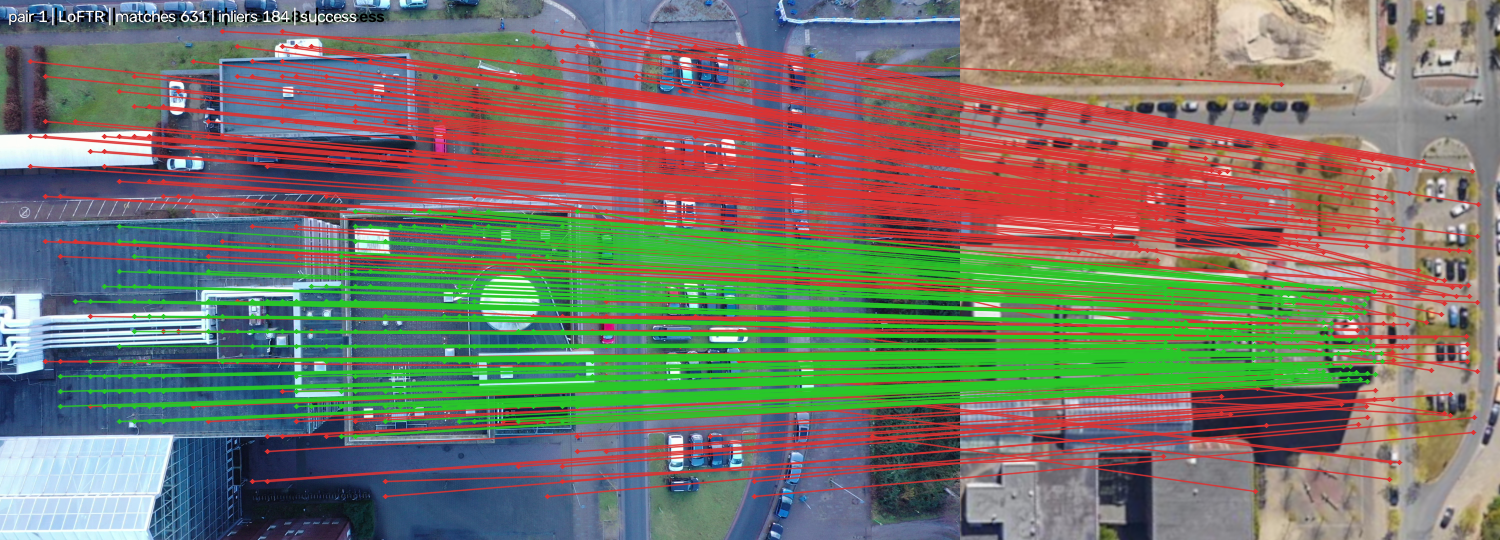
\includegraphics[width=0.92\linewidth]{images/master/pair_loftr_matches.png}
        \caption{LoFTR}
    \end{subfigure}
    \caption{Відповідності між кадром 2 (ліворуч) і фрагментом карти (праворуч): зеленим --- геометрично узгоджені, червоним --- відкинуті RANSAC}
    \label{fig:pair}
\end{figure}

\textbf{Виправлення методики курсової роботи.}\\
У курсовій роботі на цій парі LightGlue мав 229 геометрично узгоджених відповідностей проти 117 у LoFTR і працював повільніше (6,55~с проти 4,18~с). Аналіз прототипу показав, що ці результати отримано за нерівних умов. По-перше, SuperPoint неявно масштабував вхідні зображення до 1024~пікселів, тоді як LoFTR працював із 512. По-друге, обидва методи бачили лише центральну квадратну частину кадру, без нормалізації масштабу. По-третє, час вимірювався без прогрівання моделей. За однакових умов (табл.~\ref{tab:pair}) співвідношення змінюється: LoFTR знаходить удвічі більше геометрично узгоджених відповідностей за однакової їх частки, а час обробки пари на GPU для обох методів становить $\approx 0{,}25$~с. Тому числові результати курсової роботи надалі не використовуються.

\textbf{Калібрування масштабу кадру.}\\
Початкову оцінку $s_f \approx 0{,}25$ отримано вручну. Для її уточнення кадр 2 зіставлено з фрагментом карти $1024 \times 1024$, що повністю містить контур кадру. Обидва методи за обох оцінювачів і робочих масштабів $k \in \{1;\, 1{,}5\}$ дали узгоджений масштаб гомографії $\sigma = 0{,}267$--$0{,}277$, а оцінки центра кадру розійшлися не більше ніж на 16~\px{}. Отже, прийнято $s_f = 0{,}27$: кадр $1920 \times 1080$ покриває на карті ділянку $\approx 518 \times 292$~\px{}, ширшу за фрагмент 512~\px{}.

\textbf{Вплив непланарності сцени.}\\
На фрагменті 196 масштаб гомографії LoFTR ($\sigma = 0{,}20$) суттєво менший за калібрувальний (табл.~\ref{tab:pair}). Геометрично узгоджені відповідності LoFTR зосереджені на даху високої будівлі, ближчому до камери, ніж земля, тому RANSAC оцінює гомографію площини даху, а не площини землі (рис.~\ref{fig:pair}б). Центр кадру при цьому все одно визначається з похибкою $\approx 15$~\px{}, оскільки він сам розташований на цьому даху. Цей ефект є прямим наслідком припущення про плоску сцену.

\textbf{Контрольна перевірка на хибних фрагментах.}\\
Кадр 2 зіставлено з 33 фрагментами, серед яких є як сусідні до місця зйомки, так і віддалені. Фрагменти, що не перетинаються з кадром, дали щонайбільше 15 (LightGlue) і 14 (LoFTR) геометрично узгоджених відповідностей і всі були відкинуті: частина за порогом $N_{\text{in}} \ge 15$, частина --- перевіркою правдоподібності гомографії. Усі фрагменти, що перетинаються з кадром, дали від 18 до 240 таких відповідностей і пройшли перевірку. Запас між цими групами невеликий, тому для вибору фрагмента додатково використовуються частка відповідностей і умова потрапляння центра кадру у фрагмент (п.~\ref{sec:search}).

\subsection{Автоматичний пошук фрагмента для одиночного кадру}

Для кадру 2 виконано пошук без будь-якої інформації про місце зйомки (табл.~\ref{tab:search}, рис.~\ref{fig:global-loc}).

\begin{table}[H]
\centering
\caption{Автоматичний пошук фрагмента для кадру 2}
\label{tab:search}
\small
\begin{tabular}{lccccc}
\toprule
\textbf{Запуск} & \textbf{Перевірено} & \textbf{Пройшли фільтр} & \textbf{Переможець} & \textbf{Центр $(X, Y)$, \px{}} & \textbf{Час, с} \\
\midrule
LightGlue, уся карта, кеш & 384 & 5 & 220 & (1121,4;\ 2344,7) & 33 \\
LoFTR, обмежена область & 56 & 5 & 197 & (1108,6;\ 2327,5) & 18 \\
LoFTR, кожен 2-й рядок і стовпець & 96 & 1 & 197 & (1108,6;\ 2327,5) & 32 \\
\bottomrule
\end{tabular}
\end{table}

\begin{figure}[H]
    \centering
    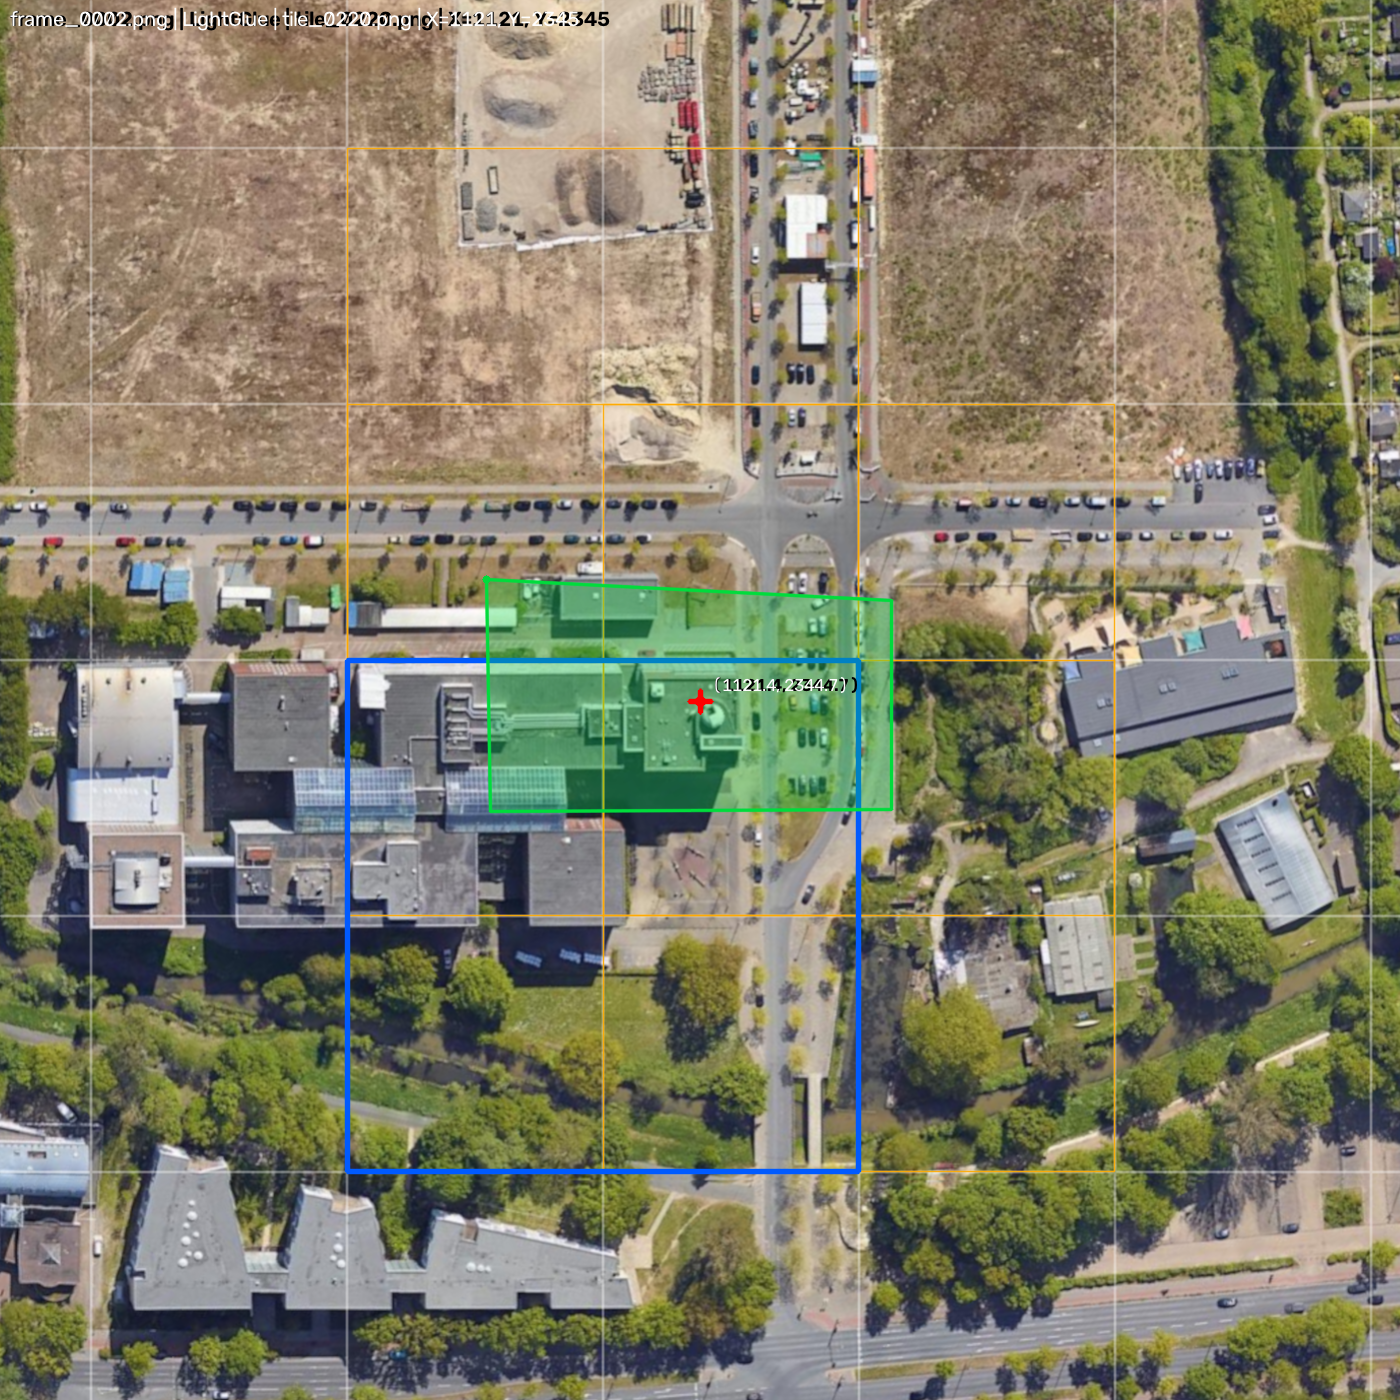
\includegraphics[width=0.75\linewidth]{images/master/global_loc_zoom.png}
    \caption{Результат автоматичного пошуку для кадру 2: сітка перевірених фрагментів, фрагменти, що пройшли фільтр (помаранчеві), фрагмент-переможець (синій), контур огляду камери (зелений) і центр кадру (червоний)}
    \label{fig:global-loc}
\end{figure}

В обох випадках переможцем став фрагмент, суміжний з еталонним фрагментом 196, який також містить центр кадру. Оцінка LoFTR відрізняється від калібрувальної оцінки $\approx(1110;\ 2330)$ на $\approx 3$~\px{}, оцінка LightGlue --- на $\approx 19$~\px{}. Усі фрагменти, що пройшли фільтр, перетинаються з місцем зйомки; жоден віддалений фрагмент фільтр не пройшов. Перегляд усієї карти з кешем ознак займає 33~с (85~мс на фрагмент), що прийнятно для початкової ініціалізації, але не для обробки кожного кадру. Це обґрунтовує використання трекера.

\subsection{Локалізація послідовності кадрів і вплив компенсації курсу}
\label{sec:exp-yaw}

Траєкторія польоту являє собою облітання кварталу: на північ, схід, південь і захід. Під час польоту курс змінюється приблизно так: $0^\circ \to 90^\circ \to 175^\circ \to -90^\circ \to -40^\circ$. Щоб оцінити внесок компенсації курсу, трекер (LightGlue + RANSAC) запущено на всіх 95 кадрах з компенсацією та без неї (табл.~\ref{tab:yaw}, рис.~\ref{fig:yaw}).

\begin{table}[H]
\centering
\caption{Вплив компенсації курсу на трекінг послідовності (LightGlue + RANSAC, 95 кадрів)}
\label{tab:yaw}
\begin{tabular}{lcc}
\toprule
& \textbf{Без компенсації} & \textbf{З компенсацією} \\
\midrule
\textsc{initialized} / \textsc{tracking} / \textsc{interpolated} / \textsc{lost} & 1 / 17 / 3 / 74 & 1 / 94 / 0 / 0 \\
Супровід утрачено & на кадрі 19, не відновлено & ні \\
Загальний час обробки & $\approx 41$~хв & 133~с \\
\bottomrule
\end{tabular}
\end{table}

\begin{figure}[H]
    \centering
    \begin{subfigure}{0.49\linewidth}
        \centering
        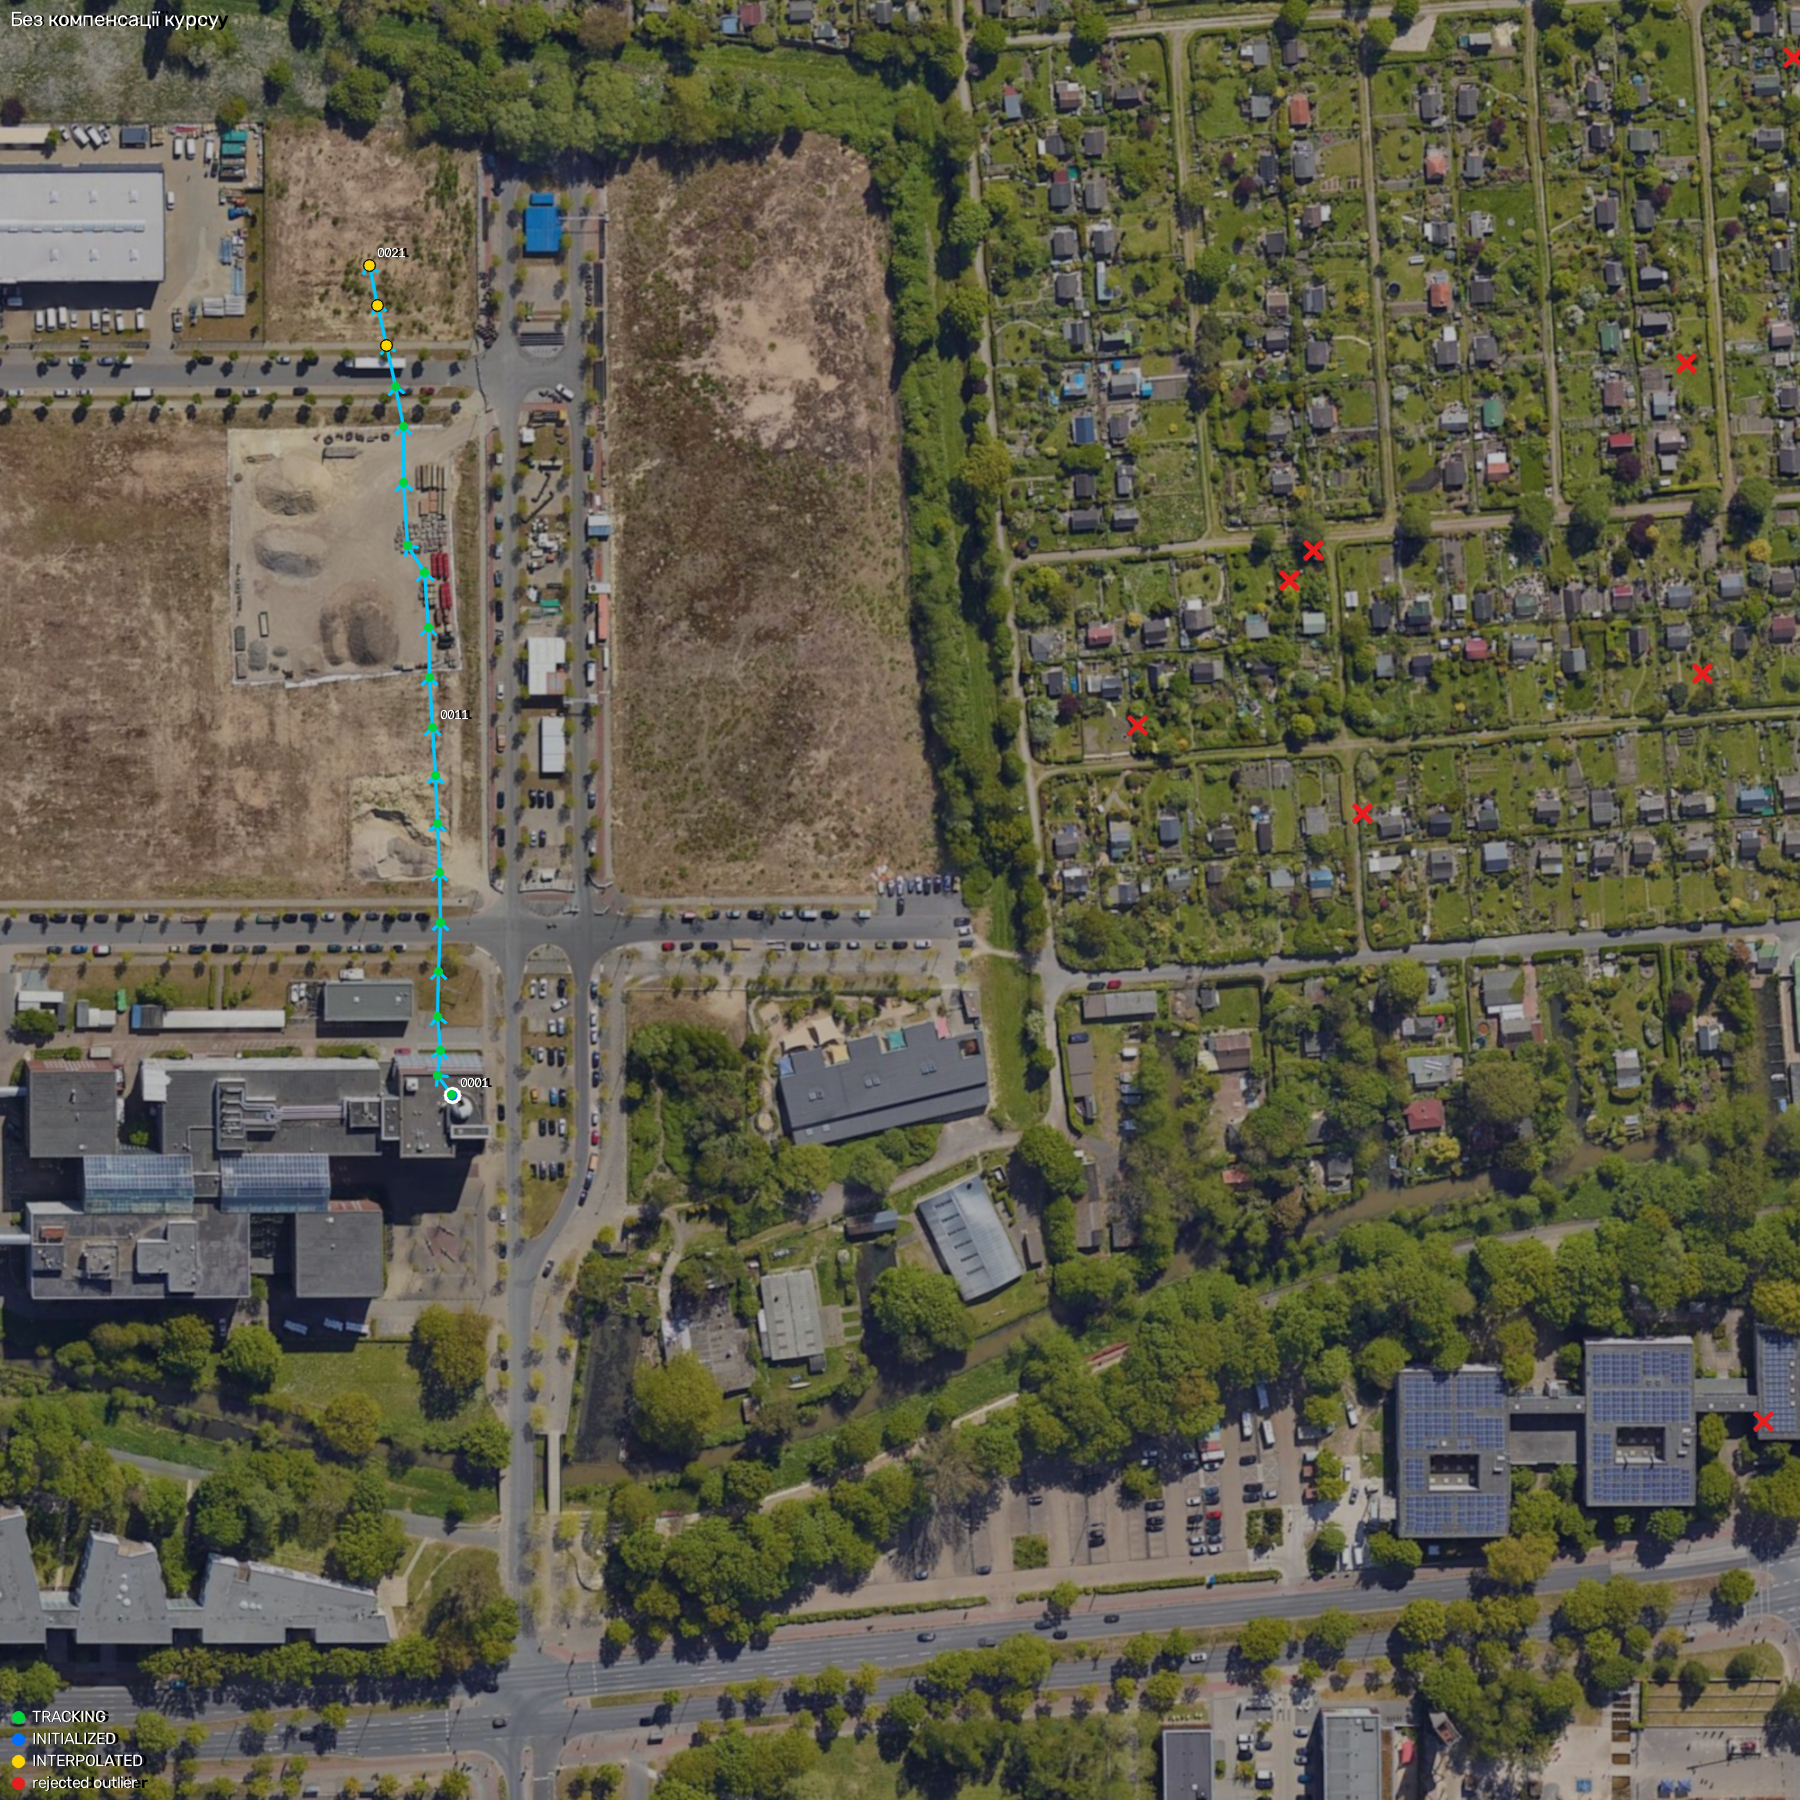
\includegraphics[width=\linewidth]{images/master/trajectory_no_yaw.png}
        \caption{без компенсації курсу}
    \end{subfigure}
    \hfill
    \begin{subfigure}{0.49\linewidth}
        \centering
        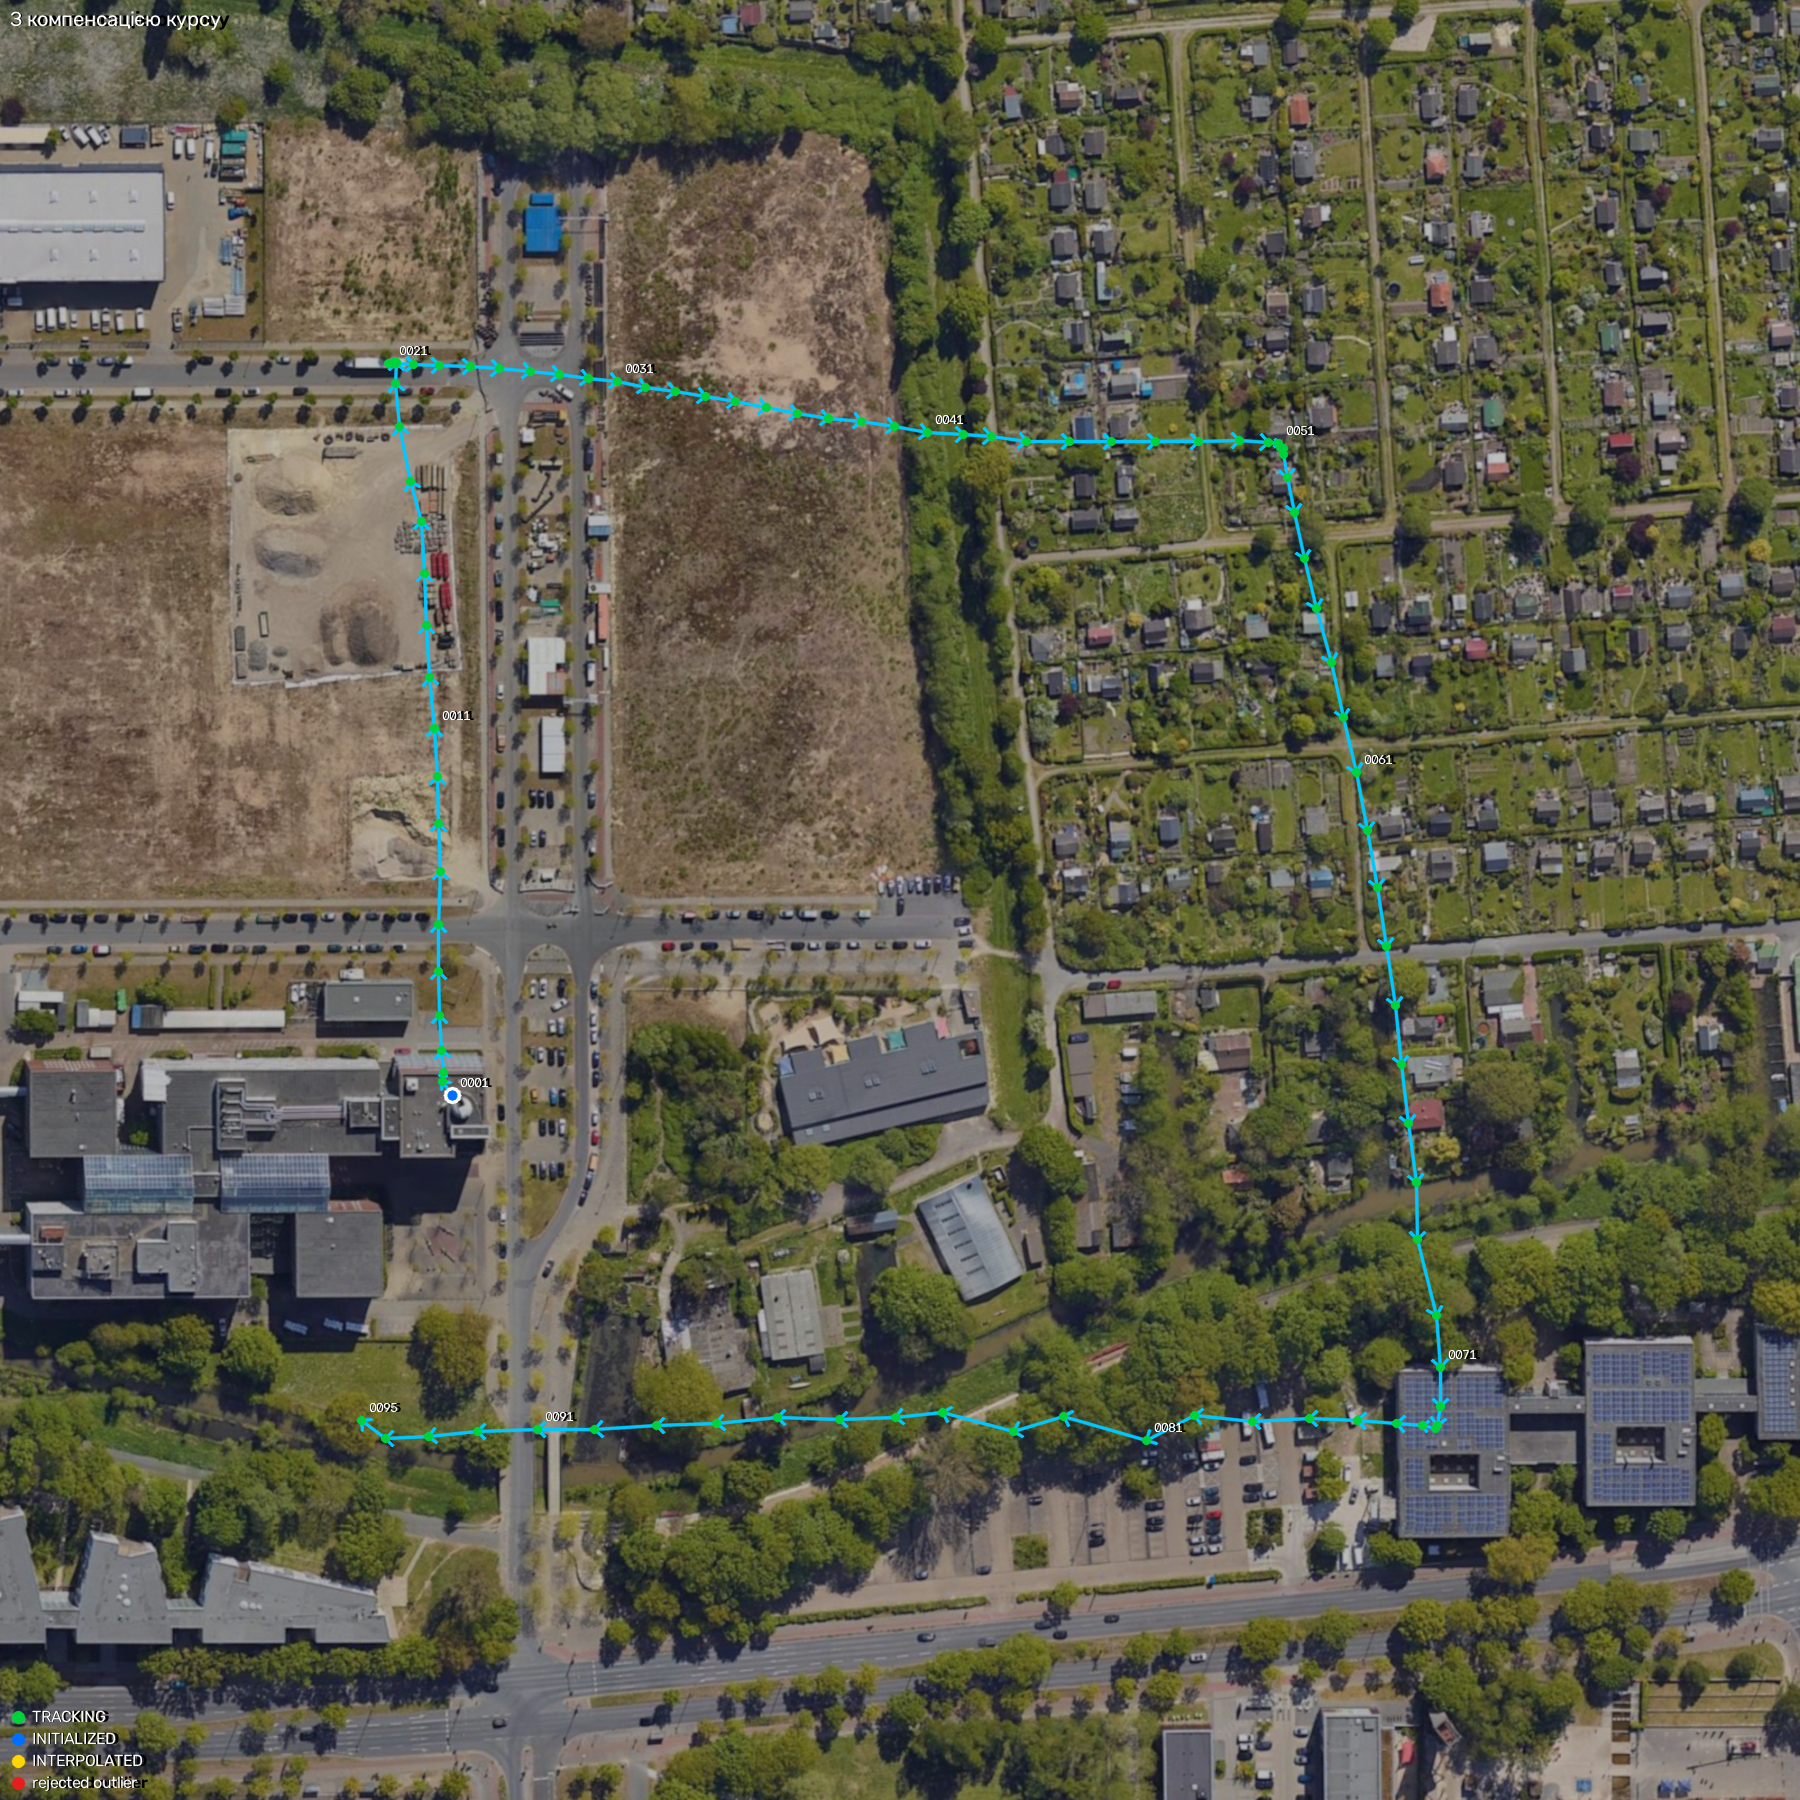
\includegraphics[width=\linewidth]{images/master/trajectory_with_yaw.png}
        \caption{з компенсацією курсу}
    \end{subfigure}
    \caption{Траєкторія, відновлена трекером: зелені точки --- \textsc{tracking}, жовті --- \textsc{interpolated}, червоні хрестики --- кандидати, відкинуті через низький бал або кінематичну перевірку}
    \label{fig:yaw}
\end{figure}

Без компенсації трекер утрачає супровід на першому розвороті (кадр 19, поворот кадру $\approx 50^\circ$). Глобальний пошук із курсом $0^\circ$ після цього вже не знаходить відповідного фрагмента. Кожен кадр у стані \textsc{lost} займає $\approx 32$~с, тому загальний час обробки зростає до 41~хв. З компенсацією всі чотири розвороти відстежено лише за прогнозом курсу; перебір додаткових гіпотез курсу знадобився для одного кадру. Компенсація курсу виявилася необхідною умовою роботи системи на реальному польоті.

\subsection{Порівняння методів LightGlue і LoFTR}
\label{sec:exp-methods}

Усі чотири конфігурації відстежили всю послідовність: 94 кадри зі статусом \textsc{tracking} і один \textsc{initialized}, лише для LightGlue + MAGSAC++ один кадр екстрапольовано. Кінематична перевірка жодного разу не відкинула оцінку, а повторна глобальна ініціалізація не знадобилася. Показники трекінгу та точності наведено в табл.~\ref{tab:tracking} і \ref{tab:accuracy}; відновлені траєкторії разом з еталоном --- на рис.~\ref{fig:traj-gt}, похибки на опорних кадрах --- на рис.~\ref{fig:error}.

\begin{table}[H]
\centering
\caption{Показники трекінгу послідовності з 95 кадрів}
\label{tab:tracking}
\small
\begin{tabular}{lcccccc}
\toprule
\multirow{2}{*}{\textbf{Конфігурація}} & \multicolumn{2}{c}{\textbf{Час кадру, с}} & \textbf{Глобальний} & \multirow{2}{*}{\textbf{Медіана} $N_{\text{in}}$} & \multirow{2}{*}{$\bar{r}$} & \multirow{2}{*}{$\bar{e}$, \px{}} \\
& середній & $P_{90}$ & \textbf{пошук, с} & & & \\
\midrule
LightGlue + RANSAC & 1,08 & 1,40 & 38,3 & 81 & 0,48 & 1,65 \\
LightGlue + MAGSAC++ & 0,78 & 1,02 & 20,1 & 87 & 0,50 & 1,73 \\
LoFTR + RANSAC & 2,72 & 2,93 & 127,9 & 316 & 0,59 & 1,27 \\
LoFTR + MAGSAC++ & 2,27 & 2,49 & 87,5 & 353 & 0,61 & 1,33 \\
\bottomrule
\end{tabular}
\end{table}

\begin{table}[H]
\centering
\caption{Похибка локалізації на 18 надійних опорних кадрах, \px{}}
\label{tab:accuracy}
\small
\begin{tabular}{lccccccc}
\toprule
\textbf{Конфігурація} & \textbf{Середня} & \textbf{Медіана} & \textbf{RMSE} & $P_{90}$ & \textbf{Макс.} & \textbf{S@10} & \textbf{S@25} \\
\midrule
LightGlue + RANSAC & 7,2 & 6,0 & 9,5 & 16,8 & 22,9 & 83\,\% & 100\,\% \\
LightGlue + MAGSAC++ & 7,5 & 5,7 & 10,2 & 16,5 & 27,5 & 78\,\% & 94\,\% \\
LoFTR + RANSAC & 4,9 & 3,1 & 7,3 & 9,0 & 24,2 & 94\,\% & 100\,\% \\
LoFTR + MAGSAC++ & 5,2 & 2,9 & 8,9 & 8,2 & 33,2 & 94\,\% & 94\,\% \\
\bottomrule
\end{tabular}
\end{table}

\begin{figure}[H]
    \centering
    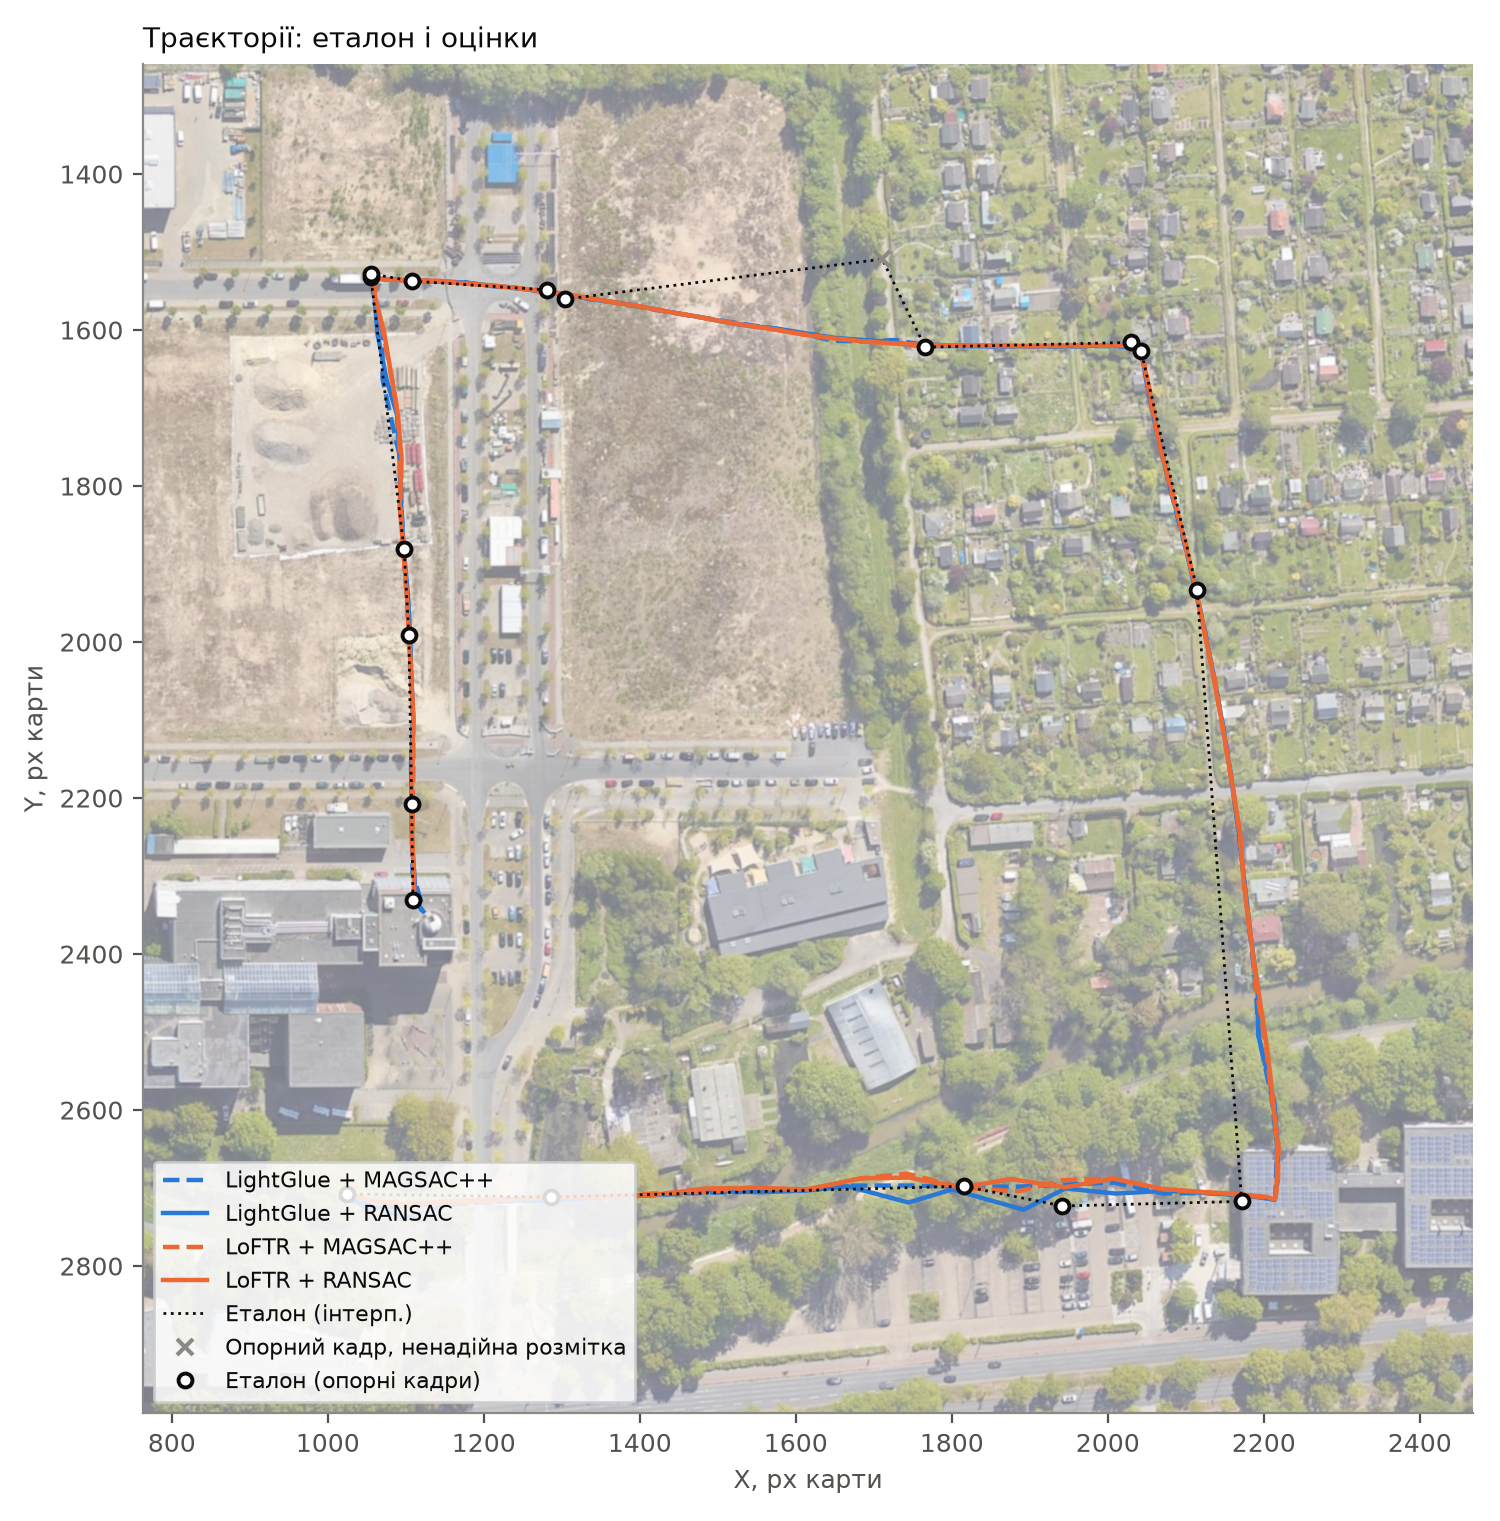
\includegraphics[width=0.8\linewidth]{images/master/trajectories_vs_gt.png}
    \caption{Траєкторії, відновлені чотирма конфігураціями, та еталонні положення опорних кадрів}
    \label{fig:traj-gt}
\end{figure}

\begin{figure}[H]
    \centering
    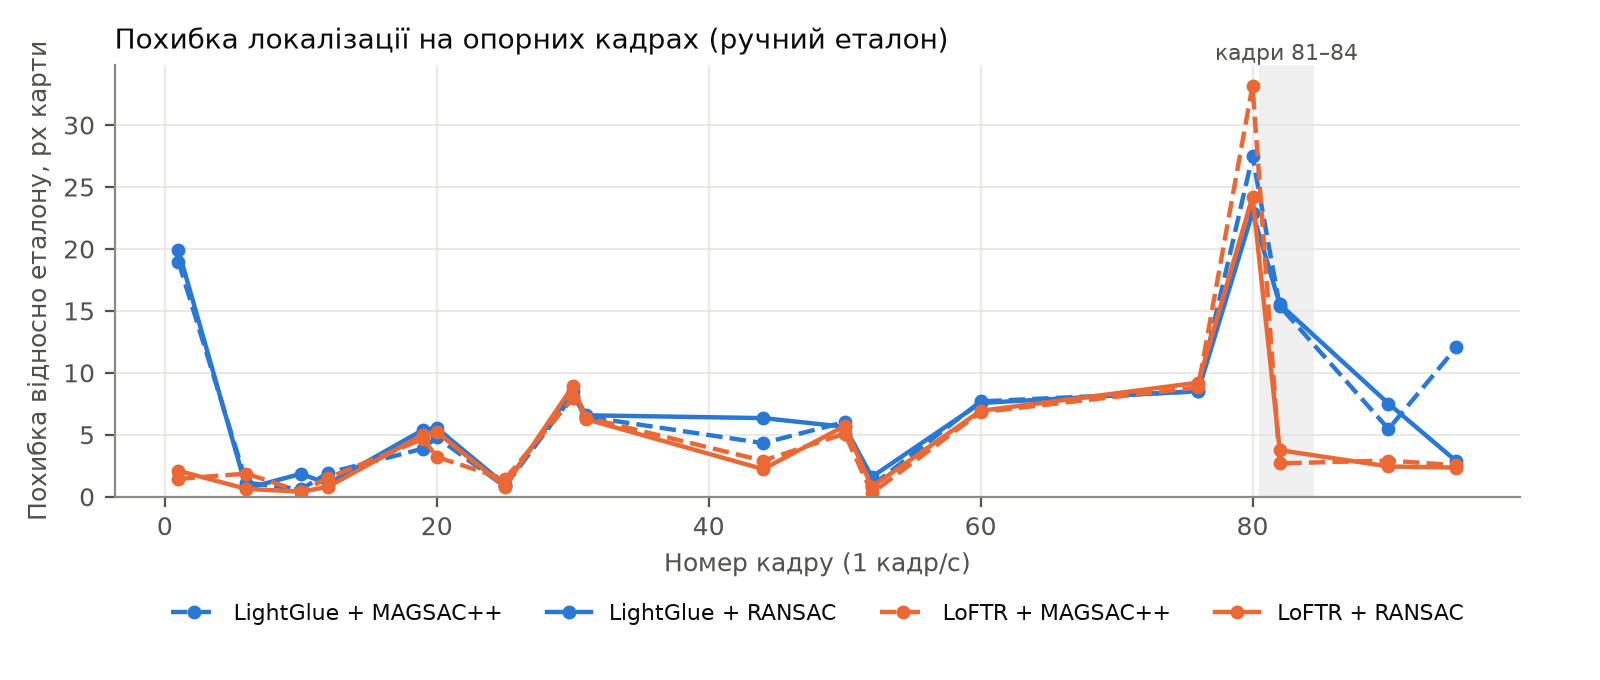
\includegraphics[width=\linewidth]{images/master/error_over_time.png}
    \caption{Похибка локалізації на опорних кадрах уздовж польоту}
    \label{fig:error}
\end{figure}

\textbf{Точність.}\\
LoFTR забезпечує меншу медіанну похибку, ніж LightGlue: $\approx 3$~\px{} проти $\approx 6$~\px{}. Частка кадрів із похибкою не більше 10~\px{} становить 94\,\% проти 78--83\,\%. У парному порівнянні з однаковим оцінювачем RANSAC LoFTR точніший на 14 з 18 опорних кадрів (знаковий тест, $p = 0{,}031$), з MAGSAC++ --- на 13 з 18 ($p = 0{,}096$). На більшості кадрів різниця між методами не перевищує 1--2~\px{}, тобто є порівнянною з невизначеністю еталона. Перевагу LoFTR формують насамперед кілька складних кадрів:
\begin{itemize}
    \item кадр 1: 19,9~\px{} у LightGlue проти 2,1~\px{} у LoFTR --- LightGlue під час ініціалізації оцінює гомографію площини даху високої будівлі (див. п.~\ref{sec:exp-pair});
    \item кадр 82 поблизу масиву дерев: 15,5~\px{} проти 3,8~\px{};
    \item кадр 90: 7,5~\px{} проти 2,4~\px{}.
\end{itemize}

На кадрі 80 усі чотири конфігурації мають близьку похибку 23--33~\px{}. Збіг похибки незалежних методів вказує на систематичну причину, спільну для всіх. Найімовірніше, це неточність еталона: усі точки розмітки цього кадру розташовані в його лівій третині (дорога й паркінг), права частина кадру зайнята деревами, а центр кадру екстрапольовано. Без кадру 80 середня похибка становить 6,2--6,3~\px{} для LightGlue і 3,6--3,7~\px{} для LoFTR; максимальна похибка LoFTR зменшується до 9,2~\px{}.

\textbf{Кількість відповідностей і швидкодія.}\\
LoFTR знаходить у 3,6--4 рази більше геометрично узгоджених відповідностей (медіана 316--353 проти 81--87) з більшою їх часткою та меншою похибкою репроєкції. Водночас LoFTR у 2,5--2,9 раза повільніший у режимі трекінгу (2,3--2,7~с проти 0,8--1,1~с на кадр) і в 3,3 (RANSAC) та 4,4 (MAGSAC++) раза повільніший під час глобального пошуку, оскільки для нього неможливе кешування ознак фрагментів. Між собою траєкторії конфігурацій відрізняються з медіаною 0,8--1,7~\px{}; найбільші розбіжності (19--43~\px{}) припадають на кадри 79--83 над деревами.

\subsection{Порівняння оцінювачів RANSAC і MAGSAC++}

Розподіл часу обробки кадру в режимі трекінгу наведено на рисунку~\ref{fig:timing}.

\begin{figure}[H]
    \centering
    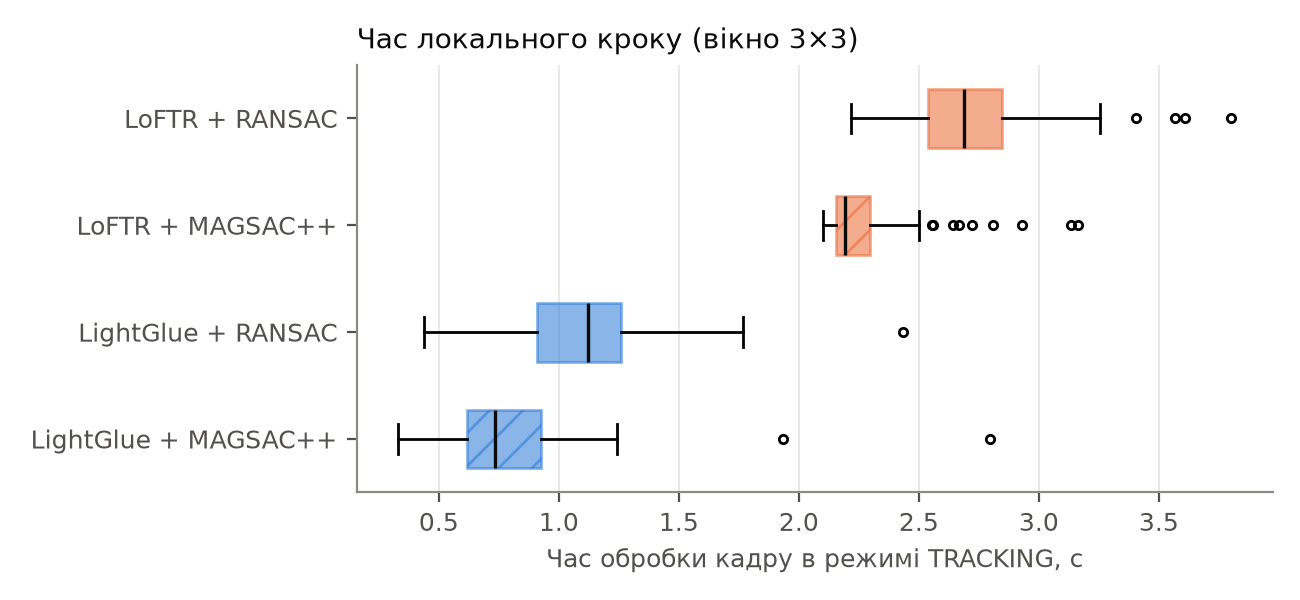
\includegraphics[width=0.75\linewidth]{images/master/timing_local.png}
    \caption{Час обробки кадру в режимі \textsc{tracking} для чотирьох конфігурацій}
    \label{fig:timing}
\end{figure}

Заміна RANSAC на MAGSAC++ скорочує час кадру на 28\,\% для LightGlue (1,08 $\to$ 0,78~с) і на 17\,\% для LoFTR (2,72 $\to$ 2,27~с), а час глобального пошуку --- у 1,9 і 1,5 раза відповідно. Виграш отримано насамперед на фрагментах, які не містять місця зйомки: на таких фрагментах реалізація RANSAC в OpenCV не може достроково зупинитися і виконує всі 5000 ітерацій, тоді як MAGSAC++ завершується за кілька мілісекунд.

Статистично значущої різниці в точності не виявлено. У парному порівнянні MAGSAC++ точніший за RANSAC на 12 з 18 кадрів для LightGlue ($p = 0{,}24$) і на 9 з 18 для LoFTR ($p = 1{,}0$), медіанна різниця не перевищує 0,2~\px{}. Траєкторії, отримані з різними оцінювачами, відрізняються з медіаною 1,2~\px{} (LightGlue) і 0,8~\px{} (LoFTR). Таким чином, MAGSAC++ дає змогу пришвидшити систему без втрати точності. Конфігурація LightGlue + MAGSAC++ --- єдина, що забезпечує обробку кадру не довше 1~с (середнє 0,78~с, $P_{90}$ 1,02~с).

\subsection{Стійкість до спотворень зображення}
\label{sec:exp-robust}

Для 19 кадрів (кожен п'ятий кадр послідовності) штучно застосовано спотворення до оригінального кадру $1920 \times 1080$:
\begin{itemize}
    \item зниження яскравості $I' = \alpha I$;
    \item зниження контрасту $I' = \alpha (I - \mu) + \mu$, де $\mu$ --- середнє значення каналу;
    \item адитивний гауссів шум;
    \item лінійне розмиття руху;
    \item поворот кадру без компенсації;
    \item помилка у заданому масштабі $s_f$.
\end{itemize}
Пул фрагментів і компенсація курсу були такими самими, як у трекері на відповідному кадрі. Для кожного кадру обчислено відношення $N_{\text{in}}$ до значення для неспотвореного кадру та зміщення знайденого центру. Результати наведено в табл.~\ref{tab:robust} і на рис.~\ref{fig:robust}.

\begin{table}[H]
\centering
\caption{Стійкість до спотворень (19 кадрів): частка локалізованих кадрів і медіанне відношення $N_{\text{in}} / N_{\text{in}}^{\text{без спотв.}}$}
\label{tab:robust}
\small
\begin{tabular}{lcccc}
\toprule
\multirow{2}{*}{\textbf{Спотворення}} & \multicolumn{2}{c}{\textbf{LightGlue}} & \multicolumn{2}{c}{\textbf{LoFTR}} \\
\cmidrule(lr){2-3}\cmidrule(lr){4-5}
& локалізовано & відношення & локалізовано & відношення \\
\midrule
яскравість $\alpha = 0{,}7$ / $0{,}5$ & 100 / 100\,\% & 1,00 / 1,01 & 100 / 100\,\% & 0,97 / 0,97 \\
контраст $\alpha = 0{,}7$ / $0{,}5$ & 100 / 100\,\% & 1,02 / 0,99 & 100 / 100\,\% & 1,00 / 0,97 \\
шум $\sigma = 10$ / $25$ & 95 / 95\,\% & 0,99 / 0,92 & 100 / 95\,\% & 1,02 / 0,95 \\
розмиття 5 / 9 пікселів & 100 / 100\,\% & 1,02 / 1,02 & 100 / 100\,\% & 1,02 / 1,04 \\
поворот $15^\circ$ / $30^\circ$ & 95 / 95\,\% & 1,03 / 0,99 & 95 / 95\,\% & 0,82 / 0,52 \\
поворот $45^\circ$ & 53\,\% & 0,35 & 11\,\% & 0 \\
поворот $90^\circ$ & 0\,\% & 0 & 0\,\% & 0 \\
масштаб $\times 0{,}8$ / $\times 1{,}25$ & 100 / 95\,\% & 0,68 / 1,29 & 100 / 100\,\% & 0,71 / 1,05 \\
\bottomrule
\end{tabular}
\end{table}

\begin{figure}[H]
    \centering
    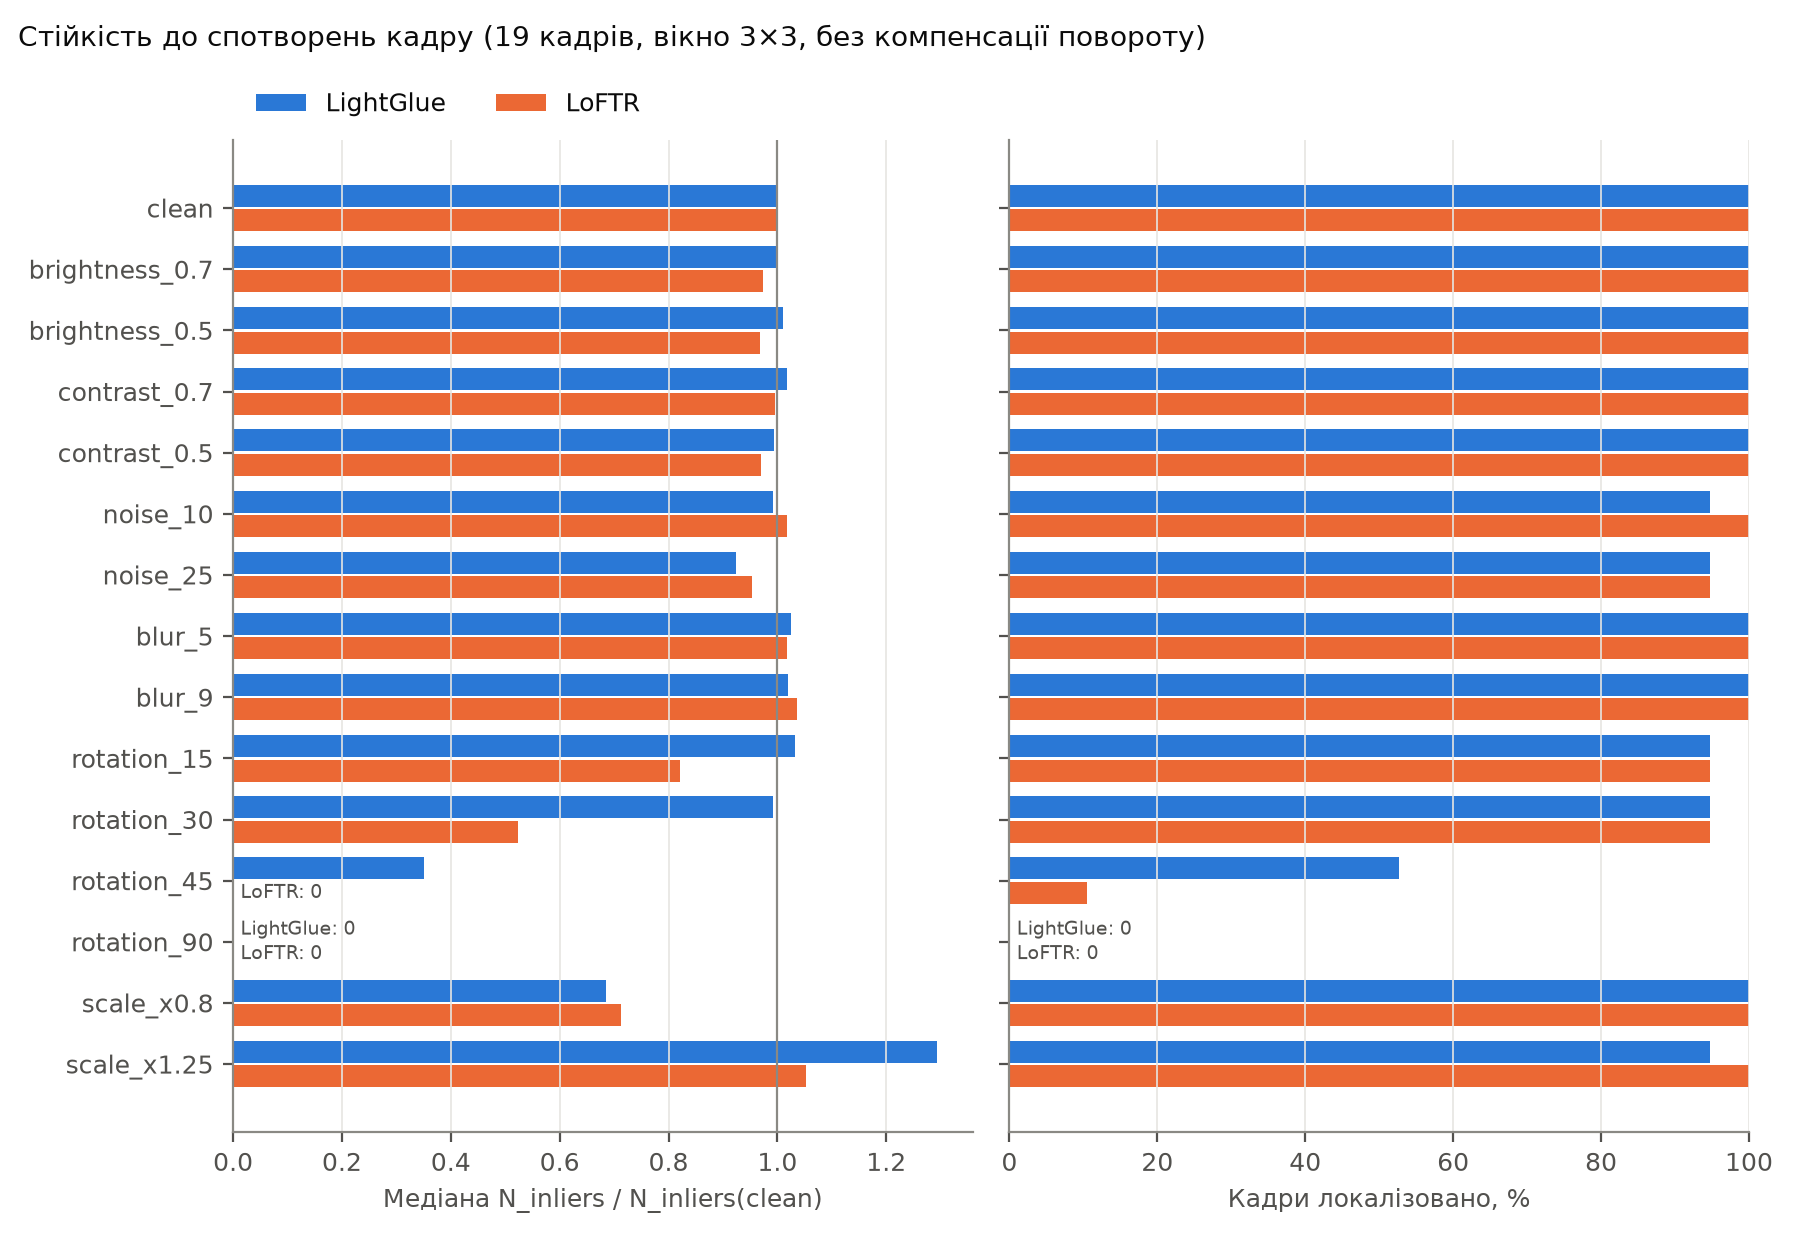
\includegraphics[width=\linewidth]{images/master/robustness.png}
    \caption{Стійкість методів до спотворень кадру}
    \label{fig:robust}
\end{figure}

Зміни яскравості й контрасту, гауссів шум і розмиття в досліджених межах практично не впливають на результат: кількість геометрично узгоджених відповідностей зберігається, а медіанне зміщення центру не перевищує 1,5~\px{}. Слабкий вплив розмиття частково пояснюється тим, що після масштабування кадру з коефіцієнтом 0,27 ядро 9 пікселів зменшується до $\approx 2{,}4$ пікселя.

Визначальним чинником виявився поворот кадру. LightGlue зберігає працездатність до $30^\circ$, а LoFTR втрачає половину відповідностей уже при $30^\circ$. При $45^\circ$ локалізовано лише 53\,\% (LightGlue) і 11\,\% (LoFTR) кадрів, при $90^\circ$ --- жодного. Ці результати кількісно обґрунтовують компенсацію курсу, описану в п.~\ref{sec:tracking}. Похибка масштабу на 20--25\,\% не призводить до втрати локалізації, але зменшення заданого масштабу на 20\,\% скорочує кількість відповідностей приблизно на 30\,\%.

\subsection{Аналіз проблемних ділянок місцевості}

Для кожного кадру за контуром огляду обчислено дві ознаки ділянки ортофотоплану:
\begin{itemize}
    \item частку рослинності за індексом Excess Green $\text{ExG} = 2g - r - b$ у хроматичних координатах \cite{exg} (піксель вважається рослинністю, якщо $\text{ExG} > 0{,}05$);
    \item текстурованість --- середній модуль градієнта Собеля яскравості.
\end{itemize}
Залежність кількості геометрично узгоджених відповідностей від номера кадру та частки рослинності наведено на рисунку~\ref{fig:terrain}, кореляції --- у табл.~\ref{tab:terrain}.

\begin{figure}[H]
    \centering
    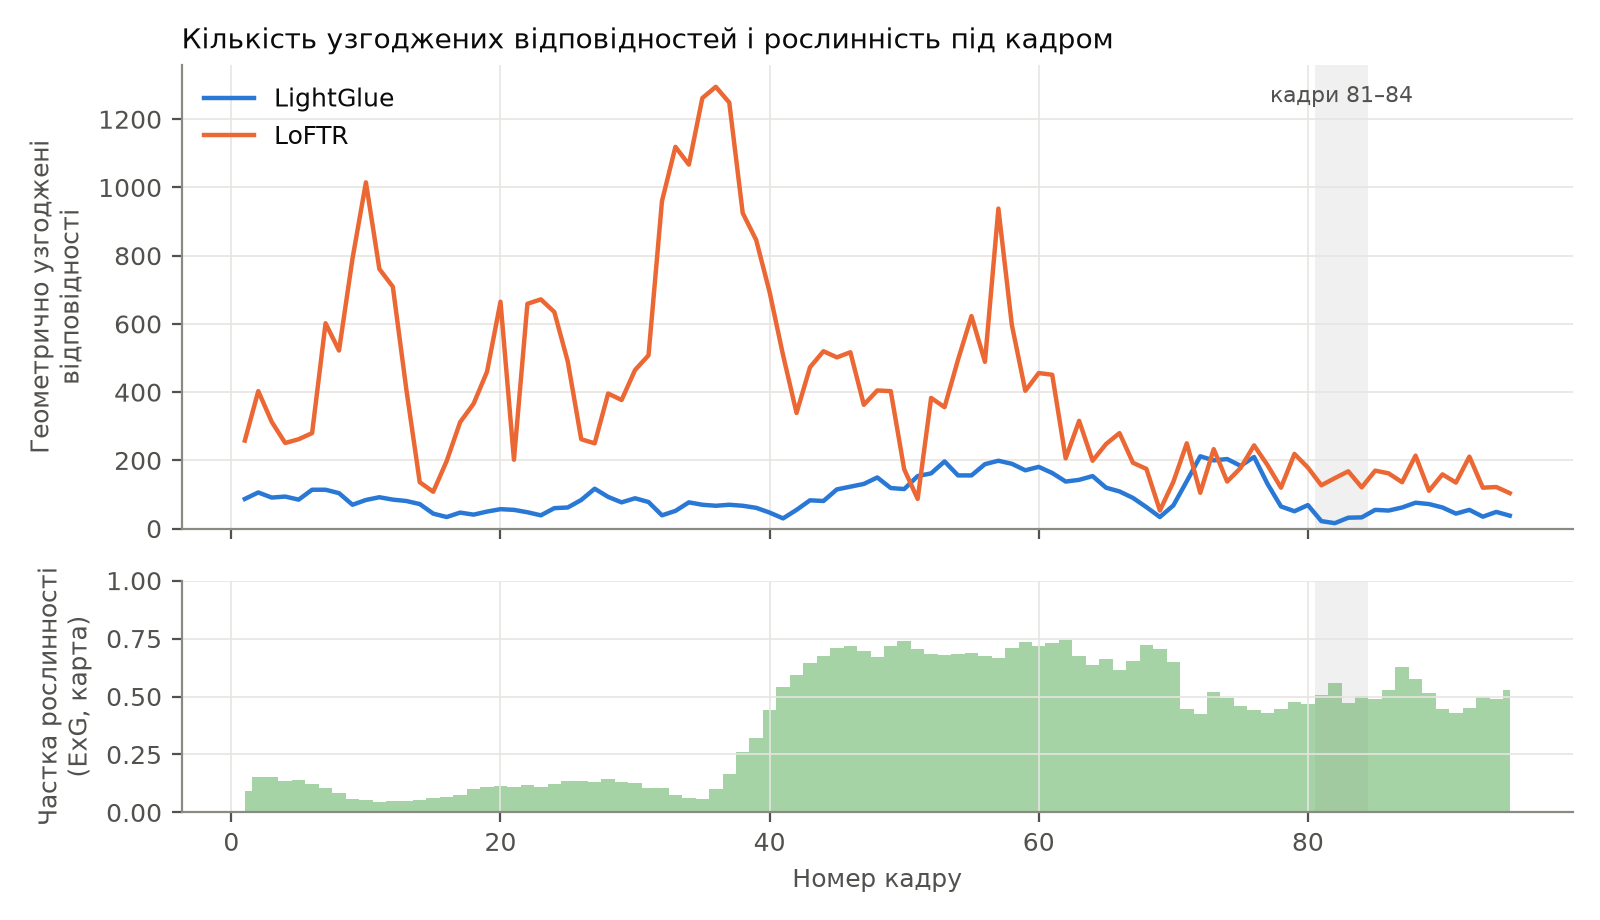
\includegraphics[width=\linewidth]{images/master/inliers_vs_terrain.png}
    \caption{Кількість геометрично узгоджених відповідностей уздовж польоту (вгорі) і частка рослинності під кадром (внизу); сірим виділено кадри 81--84}
    \label{fig:terrain}
\end{figure}

\begin{table}[H]
\centering
\caption{Зв'язок кількості геометрично узгоджених відповідностей з ознаками місцевості (кореляція Спірмена $\rho$, RANSAC)}
\label{tab:terrain}
\begin{tabular}{lcccc}
\toprule
\textbf{Метод} & $\rho$ (рослинність) & $\rho$ (текстура) & \textbf{Медіана} $N_{\text{in}}$, кадри 81--84 & \textbf{Медіана} $N_{\text{in}}$, усі \\
\midrule
LightGlue & $+0{,}37$ & $+0{,}65$ & 27 & 81 \\
LoFTR & $-0{,}29$ & $+0{,}29$ & 138 & 316 \\
\bottomrule
\end{tabular}
\end{table}

На ділянці кадрів 81--84 (паркінг і канал, оточені деревами) кількість геометрично узгоджених відповідностей падає втричі для LightGlue і вдвічі для LoFTR. Саме тут методи найбільше розходяться між собою. Водночас частка рослинності під кадром сама по собі не пояснює це падіння: для LightGlue кореляція з нею навіть додатна, оскільки дачні ділянки з будівлями мають високу частку рослинності, але багаті на деталі. Кращим предиктором для LightGlue є текстурованість ($\rho = 0{,}65$); для LoFTR зв'язок з обома ознаками слабкий. Імовірною причиною падіння на кадрах 81--84 є сезонна різниця крон листяних дерев (на відео --- без листя, на карті --- з листям), однак підтвердження цієї гіпотези потребує окремого дослідження.

% TODO: експерименти з розміром фрагмента (256/512/768/1024) і часткою перекриття (25/50 %),
%       передбачені технічним завданням, ще не проведено. Після їх виконання додати
%       підрозділ з результатами (див. обмеження нижче щодо розміру фрагмента 512).

\subsection{Обмеження розробленої системи}

Під час експериментів виявлено такі обмеження:
\begin{itemize}
    \item \textbf{Плоска модель сцени.} Гомографія описує лише площину. Високі будівлі спричиняють паралакс, і RANSAC може оцінити площину даху замість площини землі (кадр 1 у LightGlue, кадр 2 у LoFTR).
    \item \textbf{Розмір фрагмента.} Контур огляду кадру ($\approx 518 \times 292$~\px{}) ширший за фрагмент 512~\px{}, тому жоден фрагмент не містить кадр повністю.
    \item \textbf{Фіксований масштаб.} Масштаб кадру $s_f$ відкалібровано на одному кадрі, і він вважається сталим. Під час польоту оцінений масштаб гомографії змінювався в межах 0,20--0,32 (медіана 0,269), проте в трекері він не уточнюється.
    \item \textbf{Чутливість до повороту.} Без компенсації курсу обидва методи непрацездатні при повороті кадру на $45^\circ$ і більше; перший глобальний пошук виконується з курсом $0^\circ$.
    \item \textbf{Швидкодія.} Повний перебір карти займає 20--128~с залежно від конфігурації. Обмеження 1~с на кадр у режимі трекінгу на використаному GPU виконує лише LightGlue + MAGSAC++.
    \item \textbf{Одиниці вимірювання.} Без просторової прив'язки ортофотоплану похибки визначено в пікселях карти; переведення в метри потребує відомого розміру пікселя.
    \item \textbf{Обсяг даних і еталона.} Дослідження виконано на одному польоті (95 кадрів) і 18 опорних кадрах. Опорні кадри обрано за наявністю наземних орієнтирів, тому міські ділянки в еталоні представлені ширше, ніж у польоті загалом.
\end{itemize}

\subsection{Висновки за результатами експериментів}

\begin{enumerate}
    \item Розроблена система автоматично знаходить відповідний фрагмент ортофотоплану для кадру БпЛА без апріорної інформації про місце зйомки та відновлює траєкторію польоту. На послідовності з 95 кадрів усі чотири конфігурації локалізували кожен кадр без втрати супроводу.
    \item Медіанна похибка локалізації на опорних кадрах становить $\approx 3$~\px{} для LoFTR і $\approx 6$~\px{} для LightGlue; не більше ніж 10~\px{} помиляється 94\,\% і 78--83\,\% кадрів відповідно. LoFTR точніший на більшості кадрів, і його перевага найпомітніша на складних ділянках (дах високої будівлі, дерева).
    \item LightGlue у 2,5--2,9 раза швидший за LoFTR у режимі трекінгу і допускає кешування ознак карти. Конфігурація LightGlue + MAGSAC++ --- єдина, що обробляє кадр не довше 1~с (0,78~с у середньому).
    \item MAGSAC++ скорочує час обробки на 17--28\,\% без статистично значущої зміни точності, тому його доцільно використовувати замість класичного RANSAC.
    \item Обидва методи стійкі до змін яскравості, контрасту, шуму та помірного розмиття, але не до повороту кадру понад $30$--$45^\circ$. Компенсація курсу за оцінкою кута з гомографії попередніх кадрів виявилася необхідною: без неї супровід утрачається на першому розвороті.
    \item Результати курсової роботи щодо переваги LightGlue за кількістю відповідностей отримано за нерівних умов (різний масштаб вхідних зображень). За однакових умов LoFTR знаходить більше геометрично узгоджених відповідностей.
    \item Вибір методу визначається вимогами застосування: LoFTR --- для вищої точності, LightGlue + MAGSAC++ --- для обробки в реальному часі на обмеженому обладнанні.
\end{enumerate}
